\documentclass[12pt,a4paper]{IEEEtran}
\usepackage[margin=0.65in]{geometry}
\usepackage[affil-it]{authblk}
\usepackage{graphicx}
\usepackage[table,xcdraw]{xcolor}
\usepackage{caption}
\usepackage{subcaption}
\usepackage{float}
\usepackage{hyperref}
\usepackage{relsize}
\usepackage{amsmath}
{
	%	\theoremstyle{plain}
	\newtheorem{assumption}{Assumption}
}
\usepackage[most]{tcolorbox}
\tcbset{textmarker/.style={%
		enhanced,
		parbox=false,boxrule=0mm,boxsep=0mm,arc=0mm,
		outer arc=0mm,left=6mm,right=3mm,top=7pt,bottom=7pt,
		toptitle=1mm,bottomtitle=1mm}}

\newtcolorbox{importantBox}{textmarker,
	borderline west={6pt}{0pt}{red},
	colback=red!10!white}

\newcommand{\important}[1]{\begin{importantBox} \textbf{Important:} #1 \end{importantBox}}
\newcommand{\magn}[1]{\Vert{#1}\Vert}
\newcommand{\card}[1]{\vert{#1}\vert}
%\newcommand{\vbb}[2]{\vec{#1#2}}
\newcommand{\vbb}[2]{#2-#1}
%\renewcommand{\vec}[1]{\overrightarrow{#1}}
\newcommand{\pangle}{\mathit{\alpha}}
\newcommand{\leqaz}[3]{#2 \leq_{\pangle_#1} #3}
\newcommand{\angleordered}[2]{\langle #2 \rangle_{\leqaz{#1}{}{}}}
\newcommand{\prm}{\mathsf{prm}}
\newcommand{\kc}{\mathit{k_c}}
\newcommand{\kr}{\mathit{k_r}}
\newcommand{\kd}{\mathit{k_d}}
\newcommand{\kg}{\mathit{k_g}}
\newcommand{\ko}{\mathit{k_o}}
\newcommand{\rb}{\mathit{R}}

\title{Improved swarm formation through relationship-based cooordination and gap reduction in self-healing swarms.}
\author[1,*]{Neil Eliot}
\author{David Kendall}
\author{Michael Brockway}
\affil[1] {Northumbria University, Faculty of Engineering and Environment, Department of Computer and Information Sciences}
\affil[*] {Corresponding author: Dr Neil Eliot, neil.eliot@northumbria.ac.uk}
\date{\today}


\begin{document}
\maketitle

\begin{abstract}
Perimeter Compression is a technique where by a void reducing effect can be added to a basic swarming algorithm. The effect is dependant upon perimeter identification and is controlled by applying three weighting factors to the existing swarming formulae. One to the cohesion calculation, one the repulsion calculation, and one to the repulsion field size.
\end{abstract}

\section{Introduction}
When cohesion and repulsion field effects (sometimes referred to as potential fields~\cite{BAF:06,eliot2018metric,VG:05,SW:03,Son2017,liang2019swarm}) are used to create a swarming effect, the stable structures that develop are limited to either straight edges or partial lattices \cite{eliot2017methods}. The maintenance of a well-structured swarm is crucial to effective deployment for applications such as reconnaissance or artificial pollination, where `blind spots' are best eliminated \cite{elamvazhuthi2015optimal}, and containment, where the swarm is used to surround an object or region \cite{cao2012distributed}. Over time swarms form regular shapes~\cite{RAZ:13} and perimeters form of partial lattices that may contain so-called \textit{anomalies}, such as concave `dents' or convex `peaks'~\cite{eliot2019void}. These anomalies contribute to the disruption of an otherwise well-structured swarm. The key, therefore, is to ensure that these \textit{anomalies} are dynamically removed from a swarm.\\
Perimeter compression is a technique that creates a `pull' effect between perimeter agents. It is dependant upon perimeter agent identification as discussed by Eliot et. al. in \cite{eliot2017methods, eliot2018metric, eliot2019void} and discussed in Section~\ref{sec:perimeterDetection}.\\
The aim of this new algorithm is to reduce the spacing between perimeter-based agents. Figure \ref{fig:stableswarm}) shows an agent and it fields. $S$ is the sensor field. $O_b$ is the obstacle field. $C$ is the cohesion field and $\rb$ is the repulsion field. The implementation involves introducing three controlling matrices; $\kc$ which can be used to increases the magnitude of the cohesion vector. $\kr$ which can be used to modify the repulsion vector and $\rb$ which can be used to alter the repulsion fields of agents.\\

\begin{figure}[H]
	\centering
	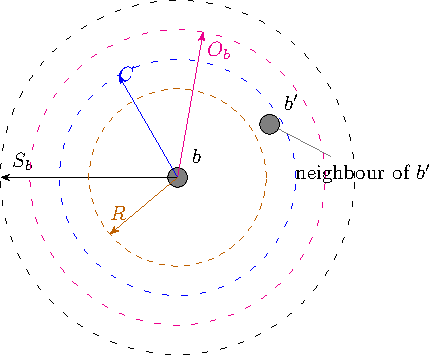
\includegraphics[width=0.8\linewidth]{figures/stableswarm}
	\caption[Agent Fields]{Agent Fields}
	\label{fig:stableswarm}
\end{figure}

\section{Related work}

As far back as 1987 swarm theory has adopted the use of field effects/potential fields to coordinate agents~\cite{REY:87} and this has continued since then in an attempt to improve the structure of a swarm, coordinate obstacle avoidance, and improve navigation~\cite{BAFVM:06,BAF:06,BFV:07,BM:09,eliot2018metric,VG:05,HC:09,SW:03,Son2017}. Improvements to the basic structure of swarms has developed through the likes of a prototype framework for self-healing swarms that was developed by Dai et al. They considered how to manage agent failure in hostile environments \cite{DHMRZ:06}. This was similar to work by Vassev and Hinchey, who modelled swarm movement using the ASSL (Autonomic System Specification Language) \cite{VH:09}. This technique was employed by NASA (US National Aeronautics and Space Administration) for use in asteroid belt exploration as part of their ANTS (Autonomous Nano Technology Swarm) project. However, this work is focused towards failure of an agent's internal systems, rather than on the removal of anomalies in a swarm distribution. This need for formation control is also discussed by Speck and Bucci with respect to the diverse applications of swarms and the need to control a swarms structure~\cite{8430773}.

In the context of swarm structure maintenance, Roach et al. focussed on the effects of sensor failure, and the impact that has on agent distribution \cite{RMT:15}. Lee and Chong identified the issue of concave edges within swarms in an attempt to create regular lattice formations \cite{GN:08}, and the main focus of their work is the dynamic restructuring of inter-agent formations. Ismail and Timmis demonstrated the use of \textit{bio-inspired} healing using \textit{granuloma formation}, a biological method for encapsulating an antigen \cite{IT:10}. They have also considered the effect failed agents can have on a swarm when traversing a terrain~\cite{TIBW:16}. 

This paper proposes an alternative approach to agent coordination that can be used to induce a void reduction effect through perimeter compression. This is an extension of the work presented by Eliot et al. \cite{eliot2019void}, Ismail and Timmis \cite{IT:10,TIBW:16}, and on the work of McLurkin and Demaine on the detection of perimeter types \cite{mclurkin2009}. However, perimeter type identification requires a communications infrastructure to allow the perimeter angle to be calculated. Communications within swarm formations limits swarm sizes and introduces performance problems \cite{fu2020formation}. The technique employed in this paper does not explicitly require the identification of the perimeter type as it would limit the size of the swarm\cite{eliot2019void,GN:08} and is therefore a reduced perimter detection algorithm to identify \textit{any} perimeter.

\section{Basic swarming model}\label{sec:basicModel}
In the Original work by Eliot et. al. the resultant vector of an agent was calculated using Equation~\ref{eq:resultantVector1a}. Where $\kc, \kr, k_d, k_o$ are weighting factors for the summed vectors associated with each interaction. i.e. $v_c$, $v_r$, $v_d$, $v_o$ for cohesion, repulsion, direction and object avoidance respectively. 

\begin{equation}\label{eq:resultantVector1a}
	v(b) = \kr v_c(b) + \kr v_r(b) + \kd v_d(b) + \ko v_o(b)
\end{equation}

Equation~\ref{eq:resultantVector1a} shows the movement vector as a linear combination of a cohesion vector $v_c$ tending to move $b$ towards its neighbours, a repulsion vector $v_r$ tending to move $b$ away from its neighbours, a direction vector  $v_d$ tending to move $b$ towards a goal, and a vector $v_o$ tending to steer it away from obstacles. $\kc, \kr, ...$ are the scalar coefficients of the the linear combination.

This paper does not consider goals or obstacles so we assume $\kd = \ko = 0$ and omit the third and fourth terms.

\subsection{Cohesion}\label{cohesion}
The cohesion component is calculated based on the proximity of neighbours. Where $n_c(b)$ is the set of neighbour agents for $b$ (Eq. \ref{eq:cohesion1}). The inclusion of an agent from a swarm ($S$) in by the agent's cohesion field ($C$).

\begin{equation}\label{eq:cohesion1}
n_c(b) = \{b' \in S~:~b' \neq b \land\magn{\vbb{b}{b'}} \leq C\}
\end{equation}

The effect of an agent being within this set is that it will generate a vector that should `encourage' agents to maintain their proximity. i.e. generate a cohesive swarm. The general weighted ($\kc$) formula for agents to maintain their proximity is to direct their motion towards the central point of all neighbouring agents as shown in Equation~\ref{eq:cohesion2}. Where $\card{n_c(b)}$ denotes the cardinality of $n_c(b)$. This formula includes the $\kc$ quotient that allows the cohesion effect to be `balanced' with respect to other vector influences as described in ~\cite{eliot2017methods,eliot2018metric,eliot2019void}. 

\begin{equation}\label{eq:cohesion2}
v_c(b) = \frac{1}{\card{n_c(b)}} \sum_{b' \in n_c(b)}(\vbb{b}{b'})
\end{equation}

\subsection{Repulsion}\label{repulsion:neighbours}
The repulsion component of an agent's movement is calculated from interaction with its neighbours $n_r(b)$ (Eq.~\ref{eq:repulsion1a}) in a swarm ($\mathcal{S}$) that are within the agent's ($b$) repulsion field ($\rb$).

\begin{equation}\label{eq:repulsion1a}
n_r(b) = \{b' \in \mathcal{S} : b \neq b' \land \card{\vbb{b}{b'}} \leq \rb)\}
\end{equation}

The repulsion is then calculated as the average of all the vectors created by the agent ($b$) to the neighbours ($b'$) (Eg.~\ref{eq:repulsion2a}) and its proximity ($\magn{\vbb{b}{b'}} - \rb$). Where $\card{n_r(b)}$ denotes the cardinality of $n_r(b)$.

\begin{equation}\label{eq:repulsion2a}
v_r(b) = \frac{1}{\card{n_r(b)}}\sum_{b' \in n_r(b)} \left(\magn{\vbb{b}{b'}} - R \, \right)\widehat{\left(\vbb{b}{b'}\right)}
\end{equation}
Here, $\widehat{\vbb{b}{b'}}$ denotes $\vbb{b}{b'}$ normalized to unit length.

\section{New Inter-agent Model}
In this paper, we propose that the behaviour of an agent should be modified depending on whether or not it is on a \emph{perimeter}. These perimeter-based agents may form part of an outer ({\color{green}green}) or inner ({\color{red}red}) boundary~(Fig.~\ref{fig:innerOuterPerimeters}). 

\begin{figure}[H]
	\begin{center}
		\includegraphics[width=5cm]{figures/PerimeterBots1}
	\end{center}
	\caption{{\color{green}Outer} and {\color{red}inner} swarm perimeters. \label{fig:innerOuterPerimeters}}
\end{figure}

\subsection{Perimeter detection}\label{sec:perimeterDetection}

The detection process is achieved using a cyclic analysis of the agents that surround an agent~(Fig.~\ref{fig:neighbours2}). Ghrist et al. discusses a similar technique using sweep angles~\cite{ghrist2008surrounding} as does McLurkin et al~\cite{mclurkin2009}. 

When detecting a perimeter it is useful to define an ordering on an agent's cohesion neighbours. We choose to order the cohesion neighbours of an agent $b$ by their \emph{polar
angle} with respect to $b$ (Fig.~\ref{fig:neighbours2}). 

\begin{figure}[H]
	\centering
	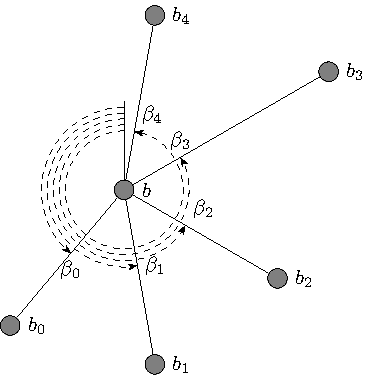
\includegraphics[width=0.8\linewidth]{figures/neighbours2}
	\caption[Agent neighbours]{Agent neighbours}
	\label{fig:neighbours2}
\end{figure}

The polar angle with respect to $b$ of $b'$,
$\pangle(b, b')$, is the counterclockwise angle that vector $\vec{bb'} = b' -
b$ makes with the positive $x$ axis as shown in Figure~\ref{fig:neighbours2} and described by Equation~\ref{eq:pangle}.

\begin{equation}\label{eq:pangle}
	\pangle(b, b') = \mathsf{atan2}((\vbb{b}{b'})_y, (\vbb{b}{b'})_x)
\end{equation} 

A partial ordering of agents by polar angle with respect to a specific agent,
$b$, is denoted $\leqaz{b}{}{}$, and is defined by: 
\begin{equation}\label{angle_ordering}
	\leqaz{b}{b'}{b''} \iff \pangle(b, b') \leq \pangle(b, b'')
\end{equation}

We denote by $\angleordered{b}{b_0, b_1, .., b_{n-1}}$ a bijection from $\{0,.., n-1\} \rightarrow n_c(b)$ that is ordered by polar angle as shown in Figure~\ref{fig:neighbours3} and more formally in Equation.~\ref{angle_polar}.
\begin{equation}\label{angle_polar}
	\forall i,
j~:~0 \leq i, j, < n \cdot i \leq j \implies \leqaz{b}{b_i}{b_j}
\end{equation}

\begin{figure}[H]
	\centering
	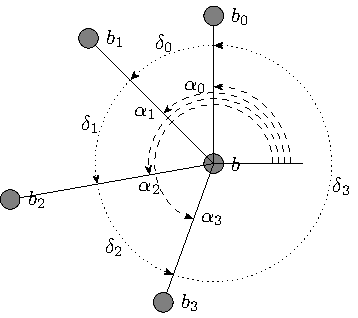
\includegraphics[width=0.8\linewidth]{figures/neighbours3}
	\caption[Agent neighbours]{Agent neighbour angles}
	\label{fig:neighbours3}
\end{figure}

An agent $b$ is on a perimeter if it satisfies any one of three conditions:
\begin{enumerate}
	\item consecutive neighbours are not within each other's cohesion field, or
	\item consecutive neighbours subtend a reflex angle, or
	\item the agent has too few neighbours.
\end{enumerate}
A function, $\prm(b)$, specifies these conditions formally. Let $b$ be the
agent of interest and $b'$, $b''$ any pair of consecutive neighbours of $b$ in
the angle-sorted list $\angleordered{b}{b_0, b_1, .., b_{n-1}}$, i.e. $b' =
b_i, b'' = b_{(i+1)\%n}$ for some $i \in \{0,..,n-1\}$.  Then $\prm(b)$ if any
one of the following conditions is satisfied:
\begin{enumerate}
\item $b' \notin n_c(b'')$,
\item $\delta > \pi$, where $\delta = \pangle(b, b'') - \pangle(b, b')$ (or $\delta = \pangle(b, b'') - \pangle(b, b') + 2\pi$ if the former is negative), or
\item $\magn{n_c(b)} < 3$.
\end{enumerate}

\subsection{$\rb$, $\kr$ and $\kc$}\label{sec:rbkrkc}

In this section we will discuss the application of the new $\rb$, $\kr$ and $\kc$ matrices which are structured as shown in Equation~\ref{eq:matrices} which are indexed via a \texttt{true} (1) / \texttt{false} (0) reference.

\begin{equation}\label{eq:matrices}
	\begin{pmatrix}
	a & b\\
	c & d
	\end{pmatrix}
\end{equation}

The new model requires each agent to modify their inter-agent repulsion and cohesion vectors based upon their perimeter status and each neighbour's perimeter status. The basic perimeter control technique is shown in Equation~\ref{eq:newModel2} where the cohesion and repulsion matrices ($\kc$, $\kr$, $\rb$) are integrated into $v_c(b)$ and $v_r(b)$.

\begin{equation}\label{eq:newModel2}
v(b) = v_c(b) + v_r(b)
\end{equation}\\

\subsubsection{Cohesion vector}
\begin{equation}\label{eq:coh2}
	v_c(b) = \frac{1}{|n_c(b)|} \sum_{b' \in n_c(b)} \kc[p_b, p_{b'}] (b' - b)
\end{equation}
where $|n_c(b)|$ denotes the cardinality of $n_c(b)$, $p_b = \prm(b)$, $p_{b'} 
= \prm(b')$, and 
$\kc$ is a 2x2 boolean-indexed array of constants that determine the weight
of a component of the cohesion vector according to
whether the interaction between $b,b'$ is between non-perimeter agents,
non-perimeter--perimeter, perimeter--non-perimeter, or perimeter--perimeter
agents.\\

\subsubsection{Repulsion vector}~\\
~\\
The set of repellers of $b$ are defined as Equation~\ref{eq:rep1}.
\small
\begin{equation}\label{eq:rep1}
	n_r(b) = \{b' \in \mathcal{S} : b \neq b' \wedge \vbb{b}{b'} \leq \rb[p_b,p_{b'}]\}
\end{equation}
\normalsize
where $p_b = \prm(b)$, $p_{b'} = \prm(b')$, and $\rb$ is a 2x2 boolean-indexed
array of constants that determine the radius of the \emph{repulsion field} for
agents in the swarm, according to whether the interaction between $b,b'$ is
between non-perimeter agents, non-perimeter--perimeter,
perimeter--non-perimeter, or perimeter--perimeter agents.

Now $v_r(b)$ is defined by Equation~\ref{eq:rep2}
\small
\begin{equation}\label{eq:rep2}
	v_r(b) = \frac{1}{\magn{n_r(b)}}\sum_{b' \in n_r(b)} \kr[p_b,p_{b'}] \left(1 - \frac{\rb[p_b,p_{b'}]}{\vbb{b}{b'}} \, \right) (\vbb{b}{b'})
\end{equation}
\normalsize
where $p_b = \prm(b)$, $p_{b'} = \prm(b')$, and $\kr$ is a 2x2 boolean-indexed
array of constants that determine the weight of a component of the repulsion
vector according to whether the interaction between $b,b'$ is between
non-perimeter agents, non-perimeter--perimeter, perimeter--non-perimeter, or
perimeter--perimeter agents.

\subsection{Gap-filling}

In addition to cohesion and repulsion vectors, a \emph{gap-filling} vector can
also be used to contribute to agent behaviour. Gap-filling vectors have proven
useful in quickly reducing internal voids and in controlling the shape of the
external perimeter.

A gap-filling vector for $b$ contributes a motion of $b$ towards the midpoint
of a gap identified in the perimeter test for $b$.

Let $\angleordered{b}{b_0, b_1, .., b_{n-1}}$ be the cohesion neighbours of $b$
in polar angle order, and let $b' = b_i$  and $b'' = b_{(i+1)\%n}$ be the first
pair of consecutive neighbours that satisfy either condition (1) or condition
(2) of the perimeter function $\prm()$, then the gap-filling vector, $v_g(b)$,
for agent $b$ is defined in Equation~\ref{eq:gap1}.
\small
\begin{equation}\label{eq:gap1}
v_g(b) = \kg \left (\frac{b' + b''}{2} - b \right) = \kg \frac{\vbb{b}{b'} + \vbb{b}{b''}}{2} 
\end{equation}
\normalsize
If there is no such pair of consecutive neighbours then $v_g(b) = 0$.

$\kg$ is a weighting for the gap-filling vector allowing the combination of it
with the other motion vectors (cohesion, repulsion, ...) to be ``tuned''.

A stricter alternative to this is to choose the first consecutive neighbour
pair $b',b''$ that satisfy condition (1), ignoring condition (2).  Again,
$v_g(b)$ is defined by eq (\ref{eq:gap1}) if such a pair exists, or 0 otherwise.

\subsection{Resultant vector}
The resultant vector is simply the sum of the cohesion, repulsion and
gap-filling vectors as shown in Equation~\ref{eq:res} and a resulant swarm segment is shown in Figure~\ref{fig:swarmExample}
\begin{equation}\label{eq:res}
	v(b) = v_c(b) + v_r(b) + v_g(b) 
\end{equation}

\begin{figure}[H]
	\begin{center}
		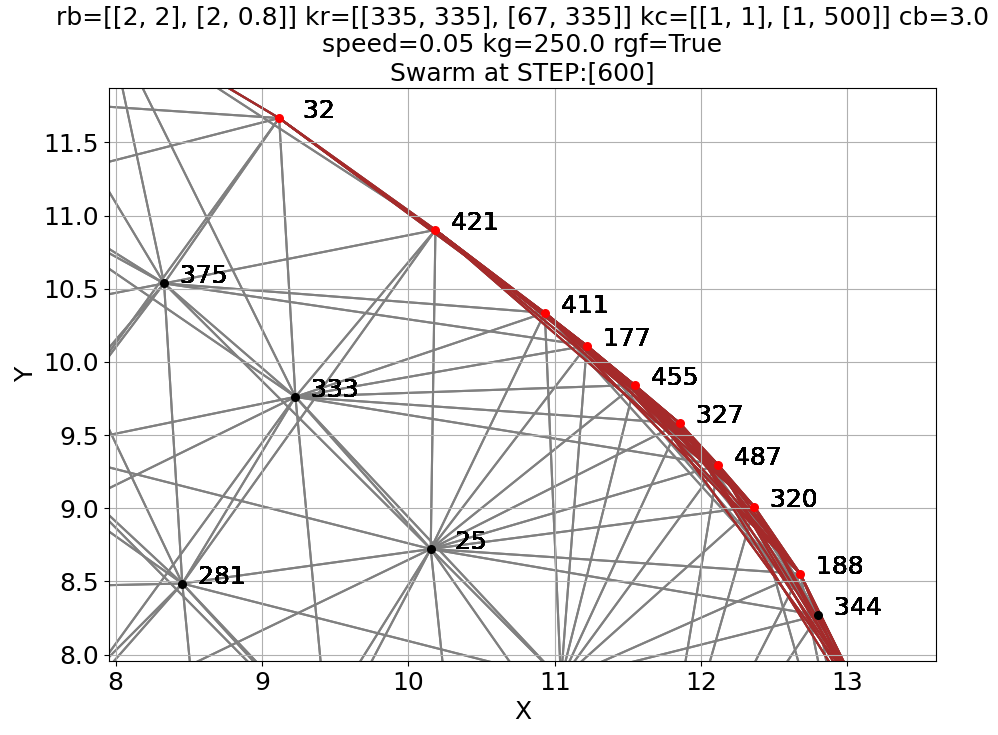
\includegraphics[width=8cm]{figures/perimeterCompress}
	\end{center}
	\caption{Swarm Example.\label{fig:swarmExample}}
\end{figure}

\subsection{Relationship-based swarm effects}

The introduction of the matrices allows for specific relationships to effect the movement of agents. Using uniform matrices results a simple cohesion/repulsion based swarm with all agents exhibiting the same properties similar to the original model discussed in \S~\ref{sec:basicModel}. However, modifying the matrices for specific relationships can induce varying effects.

\subsubsection{Cohesion model}~\\
When using Equation~\ref{eq:coh2} one matrix is used, $k_c$. This matrix is used to scale the cohesion vector generated between an agent pair which is proportional to their distance apart, which will be within $C$ as shown in Equation~\ref{eq:repulsion1a}. Consider the matrix shown in Equation~\ref{eq:kcexample1}.

\begin{equation}\label{eq:kcexample1}
	\kc = 
	\begin{pmatrix}
	1 & 1\\
	1 & 500
	\end{pmatrix}
\end{equation}

For a given agent pair their perimeter status will be calculated and applied to the matrices. If both agents are perimeter based then the value selected would be $k_c[P_b,P_{b'}]\Rightarrow 500$. If the agent pair were perimeter $\rightarrow$ non-perimeter then the value selected would be $k_c[P_b,P_{b'}]\Rightarrow 1$. This configuration would cause inter-perimeter agents to tend to move towards each other more strongly than any other relationship.

\subsubsection{Repulsion model}~\\
When using Equation~\ref{eq:rep2} two matrices are used $\kr$ and $\rb$. $\kr$ is used to scale the resultant repulsion vector that is generated. $\rb$ is the radius of the repulsion field and is used to generate the proportion of the repulsion vector that is applied. Therefore consider the following two matrices (Eqs~\ref{eq:rexample1}~and~\ref{eq:krexample1}):

\begin{equation}\label{eq:rexample1}
	\rb = 
	\begin{pmatrix}
	2 & 2\\
	2 & 0.8
	\end{pmatrix}
\end{equation}

\begin{equation}\label{eq:krexample1}
	\kr = 
	\begin{pmatrix}
	335 & 335\\
	67 & 335
	\end{pmatrix}
\end{equation}

For a given agent pair their perimeter status will be calculated and applied to the matrices. If both agents are perimeter based then the values selected would be $\rb[P_b,P_{b'}]\Rightarrow 0.8$ and $\kr[P_b,P_{b'}]\Rightarrow 335$. If the agent pair were perimeter $\rightarrow$ non-perimeter then the values selected would be $\rb[P_b,P_{b'}]\Rightarrow 2$ and $\kr[P_b,P_{b'}]\Rightarrow 67$.\\


==== STILL TO BE WORKED ON =====\\
\section{Experimental results\label{sec:ExperimentalResults}}
\subsection{Baseline}
For all the experiments the parameters used to create the basic swarming effect are shown in Table~\ref{tab:swarmingEffect}. Where $C$ is the cohesion field, $k_c$ is the cohesion weighting, $R_b$ is the repulsion field, $k_r$ is the repulsion weighting and $k_g$ is the weighting factor applied in the comparison of the gap reduction algorithm discussed in~\cite{eliot2019void}. The swarm consists of 200 agents which are distributed with a void at the centre. These initial parameters create a hexagonal-based distribution of agents that stabilise as shown in Figure~\ref{fig:baselineSwarm}. This basic swarm is used as the initial state for all the experiments. 
 \begin{table}[ht]
	\centering
	\tiny
	\begin{tabular}{|c|r|}
		\hline
		\rowcolor[HTML]{000000} 
		{\color[HTML]{FFFFFF} Swarming Variable} & {\color[HTML]{FFFFFF} Value} \\ \hline
		$C_b$ & \texttt{3.00} \\ \hline
		$k_c$ & \texttt{0.15}  \\ \hline
		$R_b$ & \texttt{2.00} \\ \hline
		$k_r$ & \texttt{50.00} \\ \hline
		$k_g$ & \texttt{25.00} \\ \hline
	\end{tabular}
  	\caption{Swarming effect parameters}
  	\label{tab:swarmingEffect}
\end{table}

\begin{figure}[H]
	\begin{center}
		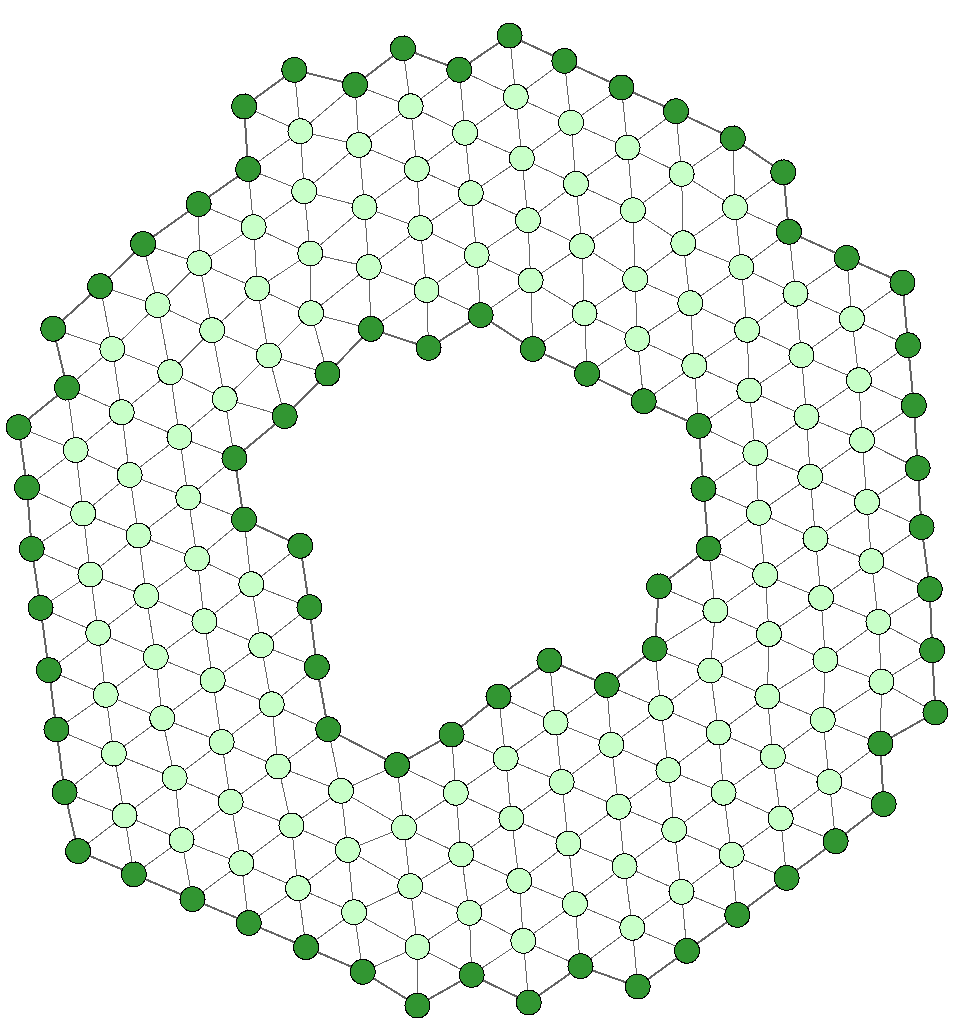
\includegraphics[width=5cm]{figures/exp1Start}
	\end{center}
	\caption{Baseline swarm in stabilised configuration. \label{fig:baselineSwarm}}
\end{figure}

When the simulation is ran with no compression the changes are identified using a magnitude-based metric~\cite{eliot2018metric}. The resultant magnitudes generated are shown in figure~\ref{fig:baselineSwarmMagnitude}. These states are used as the baseline for the experiments to measure the effects of the compression algorithm and compare the new algorithm to the existing void reduction algorithm.

\begin{figure}[ht]
	\begin{center}
		\includegraphics[width=8cm]{figures/interagentMagnitudeBaseline}
	\end{center}
	\caption{Baseline swarm in stabilised configuration. \label{fig:baselineSwarmMagnitude}}
\end{figure}



Figure~\ref{fig:voidRemoval} shows how the compression effect can remove a void from a swarm by surround an obstacle in a similar manner to the method described in~\cite{eliot2019void}.

\begin{figure}[ht]
	\centering
	\begin{subfigure}{0.4\textwidth}
		\centering	
		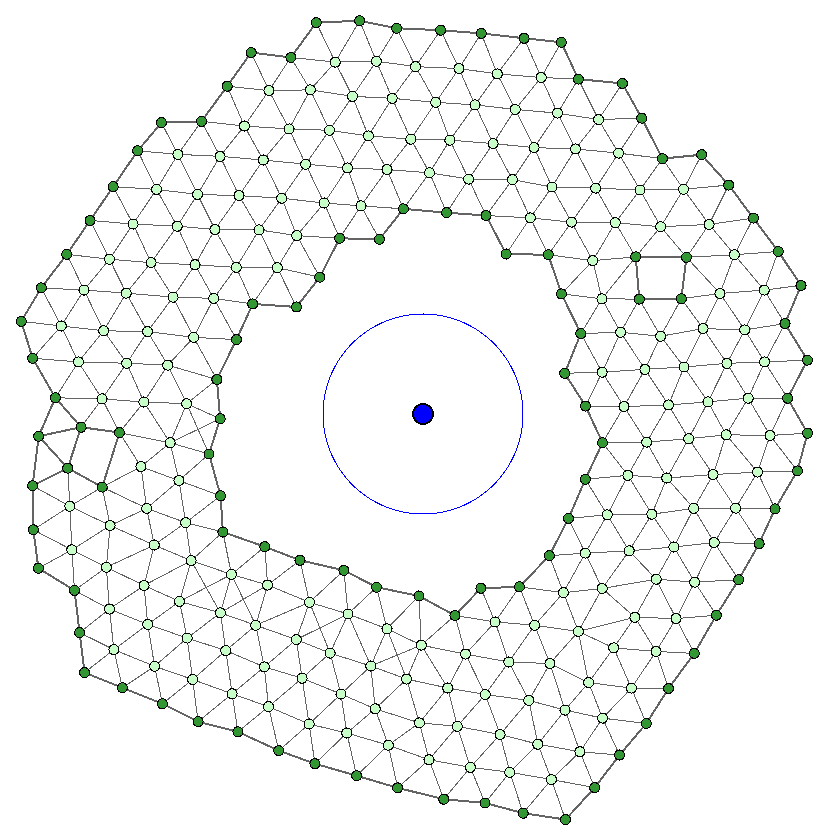
\includegraphics[width=1.0\linewidth]{figures/voidRemoval1}
		\caption[Void removal start]{Void removal start}
		\label{fig:voidRemovalStart}
	\end{subfigure}
	\begin{subfigure}{0.4\textwidth}
		\centering
		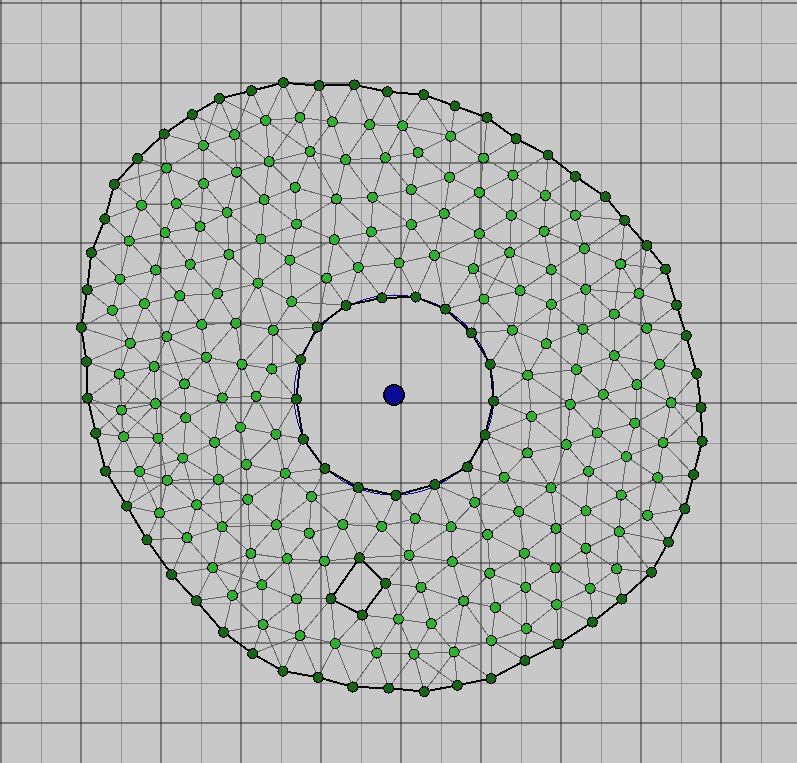
\includegraphics[width=1.0\linewidth]{figures/voidRemoval2}
		\caption[Void removal finish]{Void removal finish}
		\label{fig:voidRemovalFinish}
	\end{subfigure}
	\caption{Void removal through perimeter compression}
	\label{fig:voidRemoval}
\end{figure}

\subsection{Inner compression model}

\begin{equation}
p_{kr} = \left (
\begin{array}{cc}
1 & x\\
1 & 1
\end{array} \right )
\end{equation}

\begin{equation}
p_{kc} = \left (
\begin{array}{cc}
1 & y\\
1 & 1
\end{array} \right )
\end{equation}

\subsubsection{Inner + Gap compression model}

\subsection{Outer compression model}

\begin{equation}
p_{kr} = \left (
\begin{array}{cc}
1 & x\\
x & 1
\end{array} \right )
\end{equation}

\begin{equation}
p_{kc} = \left (
\begin{array}{cc}
1 & y\\
y & 1
\end{array} \right )
\end{equation}

\subsubsection{Outer + Gap compression model}


\subsection{Compression Effects\label{sec:CompressionEffect}}

The compression effect parameters are shown in tables~\ref{tab:compressionExperimentEffect1} and~\ref{tab:compressionExperimentEffect2}

\begin{table}[ht]
	\centering
	\tiny
\begin{tabular}{ | >{\columncolor[HTML]{000000}}l | l | l | l | l | l | }
	\hline
	\rowcolor[HTML]{000000} 
	{\color[HTML]{FFFFFF} Pr/Pc} & {\color[HTML]{FFFFFF}10} & {\color[HTML]{FFFFFF}20} & {\color[HTML]{FFFFFF}30} & {\color[HTML]{FFFFFF}40} & {\color[HTML]{FFFFFF}50} \\ \hline
	    {\color[HTML]{FFFFFF}0.1} & 0.1/10 & 0.1/20 & 0.1/30 & 0.1/40 & 0.1/50  \\ \hline
		{\color[HTML]{FFFFFF}0.2} & 0.2/10 & 0.2/20 & 0.2/30 & 0.2/40 & 0.2/50  \\ \hline
		{\color[HTML]{FFFFFF}0.3} & 0.3/10 & 0.3/20 & 0.3/30 & 0.3/40 & 0.3/50  \\ \hline
		{\color[HTML]{FFFFFF}0.4} & 0.4/10 & 0.4/20 & 0.4/30 & 0.4/40 & 0.4/50  \\ \hline
		{\color[HTML]{FFFFFF}0.5} & 0.5/10 & 0.5/20 & 0.5/30 & 0.5/40 & 0.5/50  \\ \hline
		{\color[HTML]{FFFFFF}0.6} & 0.6/10 & 0.6/20 & 0.6/30 & 0.6/40 & 0.6/50  \\ \hline
		{\color[HTML]{FFFFFF}0.7} & 0.7/10 & 0.7/20 & 0.7/30 & 0.7/40 & 0.7/50  \\ \hline
		{\color[HTML]{FFFFFF}0.8} & 0.8/10 & 0.8/20 & 0.8/30 & 0.8/40 & 0.8/50  \\ \hline
		{\color[HTML]{FFFFFF}0.9} & 0.9/10 & 0.9/20 & 0.9/30 & 0.9/40 & 0.9/50  \\ \hline
	\end{tabular}
	\caption{Experiment parameters 1}
	\label{tab:compressionExperimentEffect1}
\end{table}

\begin{table}[ht]
	\centering
	\tiny
\begin{tabular}{ | >{\columncolor[HTML]{000000}}l | l | l | l | l | l | }
	\hline
	\rowcolor[HTML]{000000} 
	{\color[HTML]{FFFFFF} Pr/Pc} & {\color[HTML]{FFFFFF}60} & {\color[HTML]{FFFFFF}70} & {\color[HTML]{FFFFFF}80} & {\color[HTML]{FFFFFF}90} & {\color[HTML]{FFFFFF}100}   \\ \hline
		{\color[HTML]{FFFFFF}0.1} & 0.1/60 & 0.1/70 & 0.1/80 & 0.1/90 & 0.1/100 \\ \hline
		{\color[HTML]{FFFFFF}0.2} & 0.2/60 & 0.2/70 & 0.2/80 & 0.2/90 & 0.2/100 \\ \hline
		{\color[HTML]{FFFFFF}0.3} & 0.3/60 & 0.3/70 & 0.3/80 & 0.3/90 & 0.3/100 \\ \hline
		{\color[HTML]{FFFFFF}0.4} & 0.4/60 & 0.4/70 & 0.4/80 & 0.4/90 & 0.4/100 \\ \hline
		{\color[HTML]{FFFFFF}0.5} & 0.5/60 & 0.5/70 & 0.5/80 & 0.5/90 & 0.5/100 \\ \hline
		{\color[HTML]{FFFFFF}0.6} & 0.6/60 & 0.6/70 & 0.6/80 & 0.6/90 & 0.6/100 \\ \hline
		{\color[HTML]{FFFFFF}0.7} & 0.7/60 & 0.7/70 & 0.7/80 & 0.7/90 & 0.7/100 \\ \hline
		{\color[HTML]{FFFFFF}0.8} & 0.8/60 & 0.8/70 & 0.8/80 & 0.8/90 & 0.8/100 \\ \hline
		{\color[HTML]{FFFFFF}0.9} & 0.9/60 & 0.9/70 & 0.9/80 & 0.9/90 & 0.9/100 \\ \hline
	\end{tabular}
	\caption{Experiment parameters 2}
	\label{tab:compressionExperimentEffect2}
\end{table}

\begin{figure}[H]
	\begin{center}
		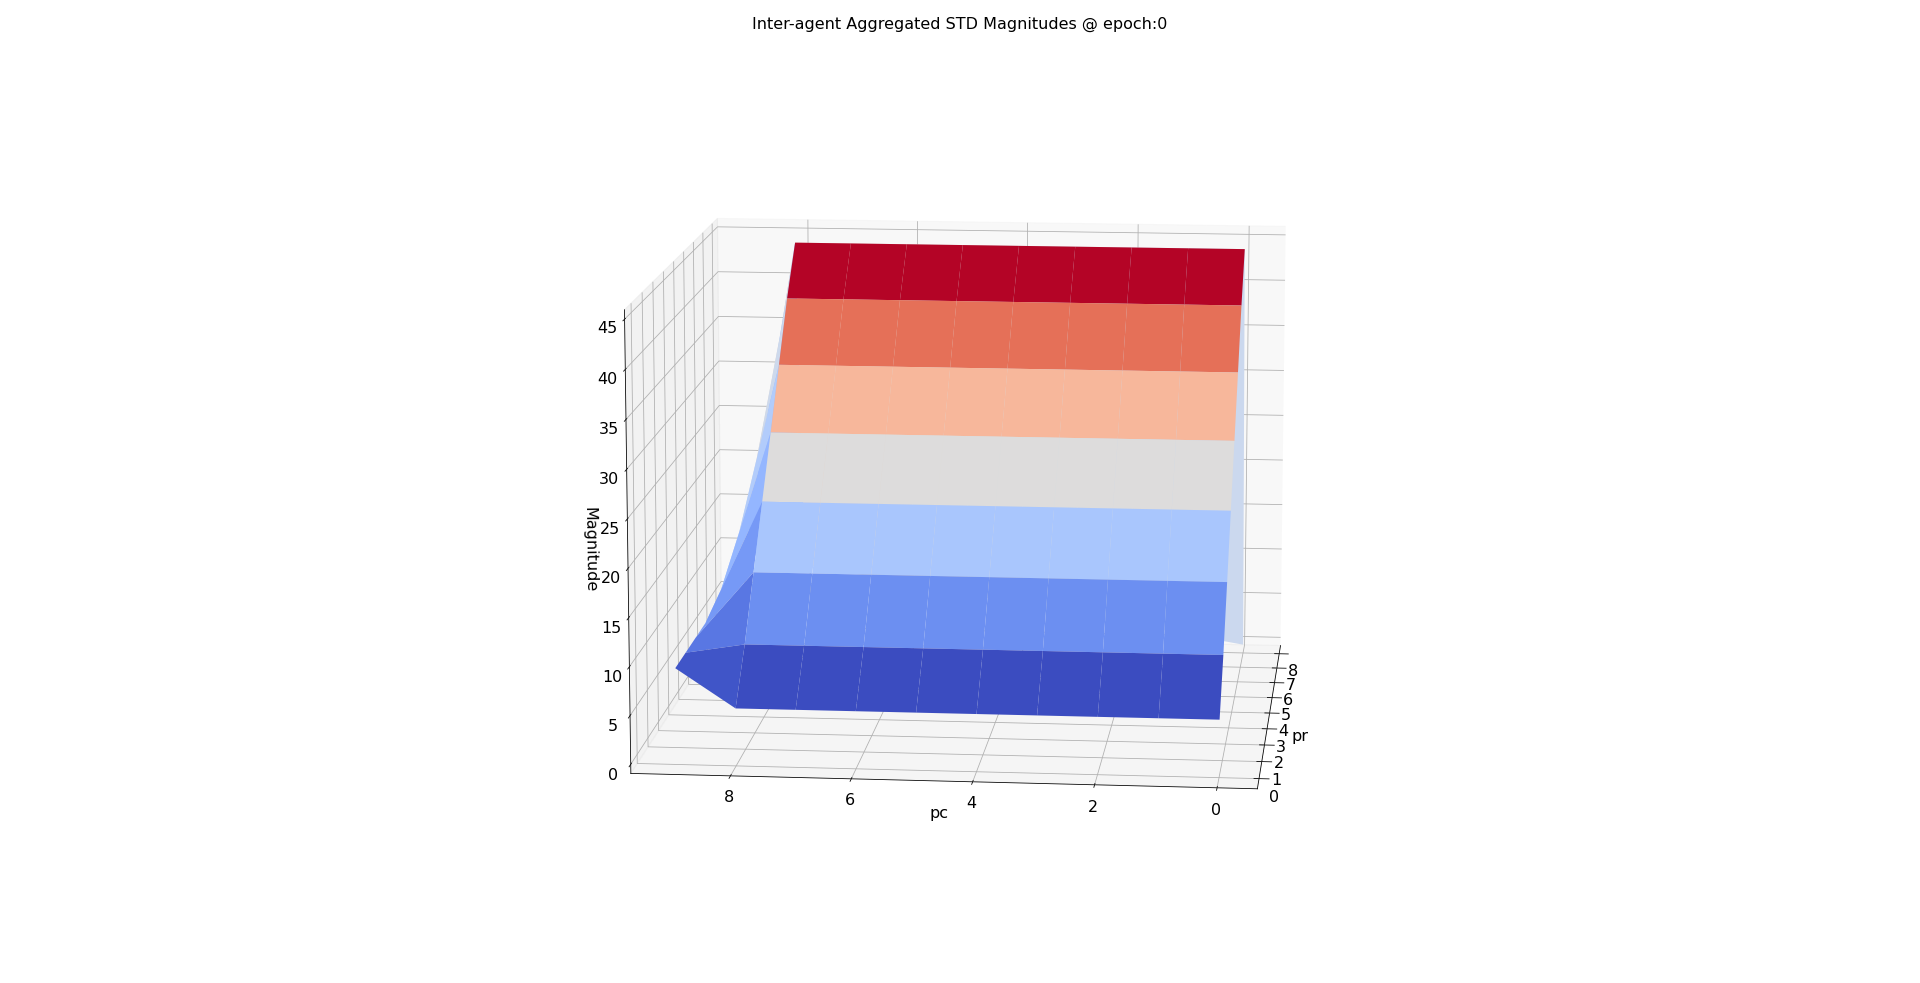
\includegraphics[width=8cm]{figures/Experiment1}
	\end{center}
	\caption{Experiment Start \label{fig:experiment1}}
\end{figure}

\begin{figure}[H]
	\begin{center}
		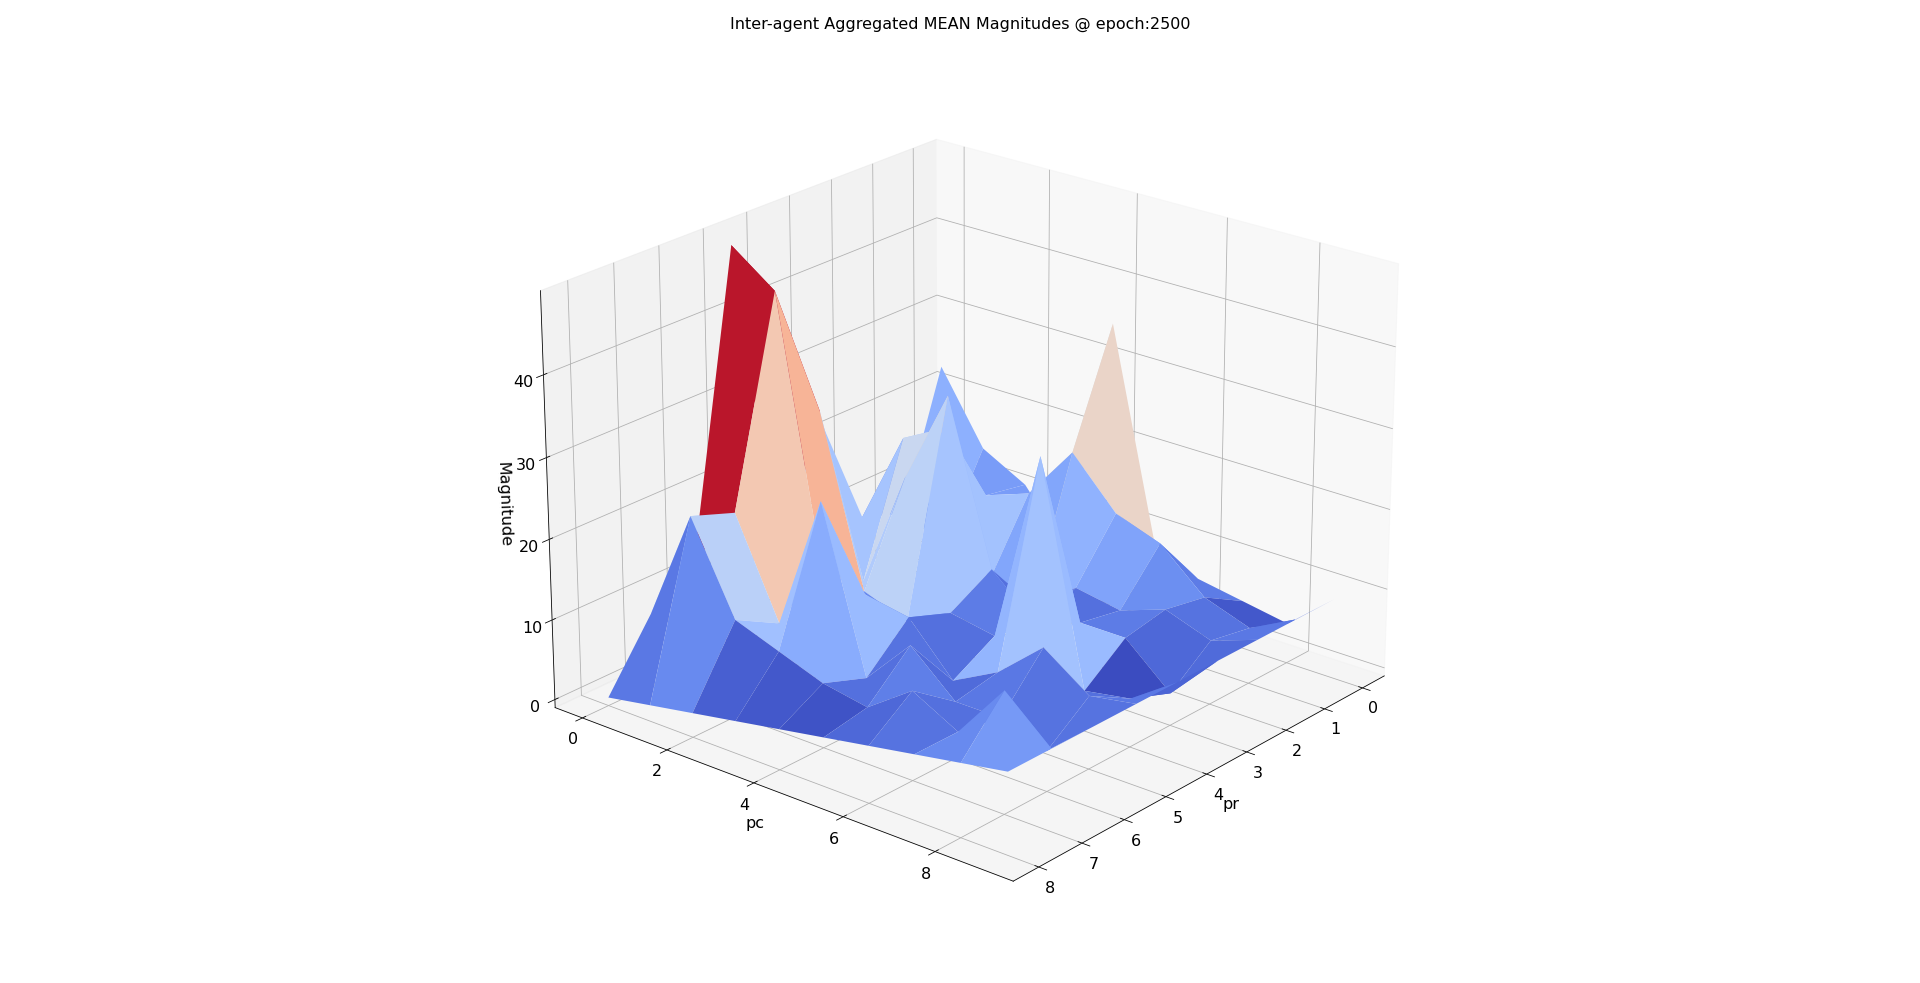
\includegraphics[width=8cm]{figures/Experiment2}
	\end{center}
	\caption{Experiment Middle \label{fig:experiment2}}
\end{figure}

\begin{figure}[H]
	\begin{center}
		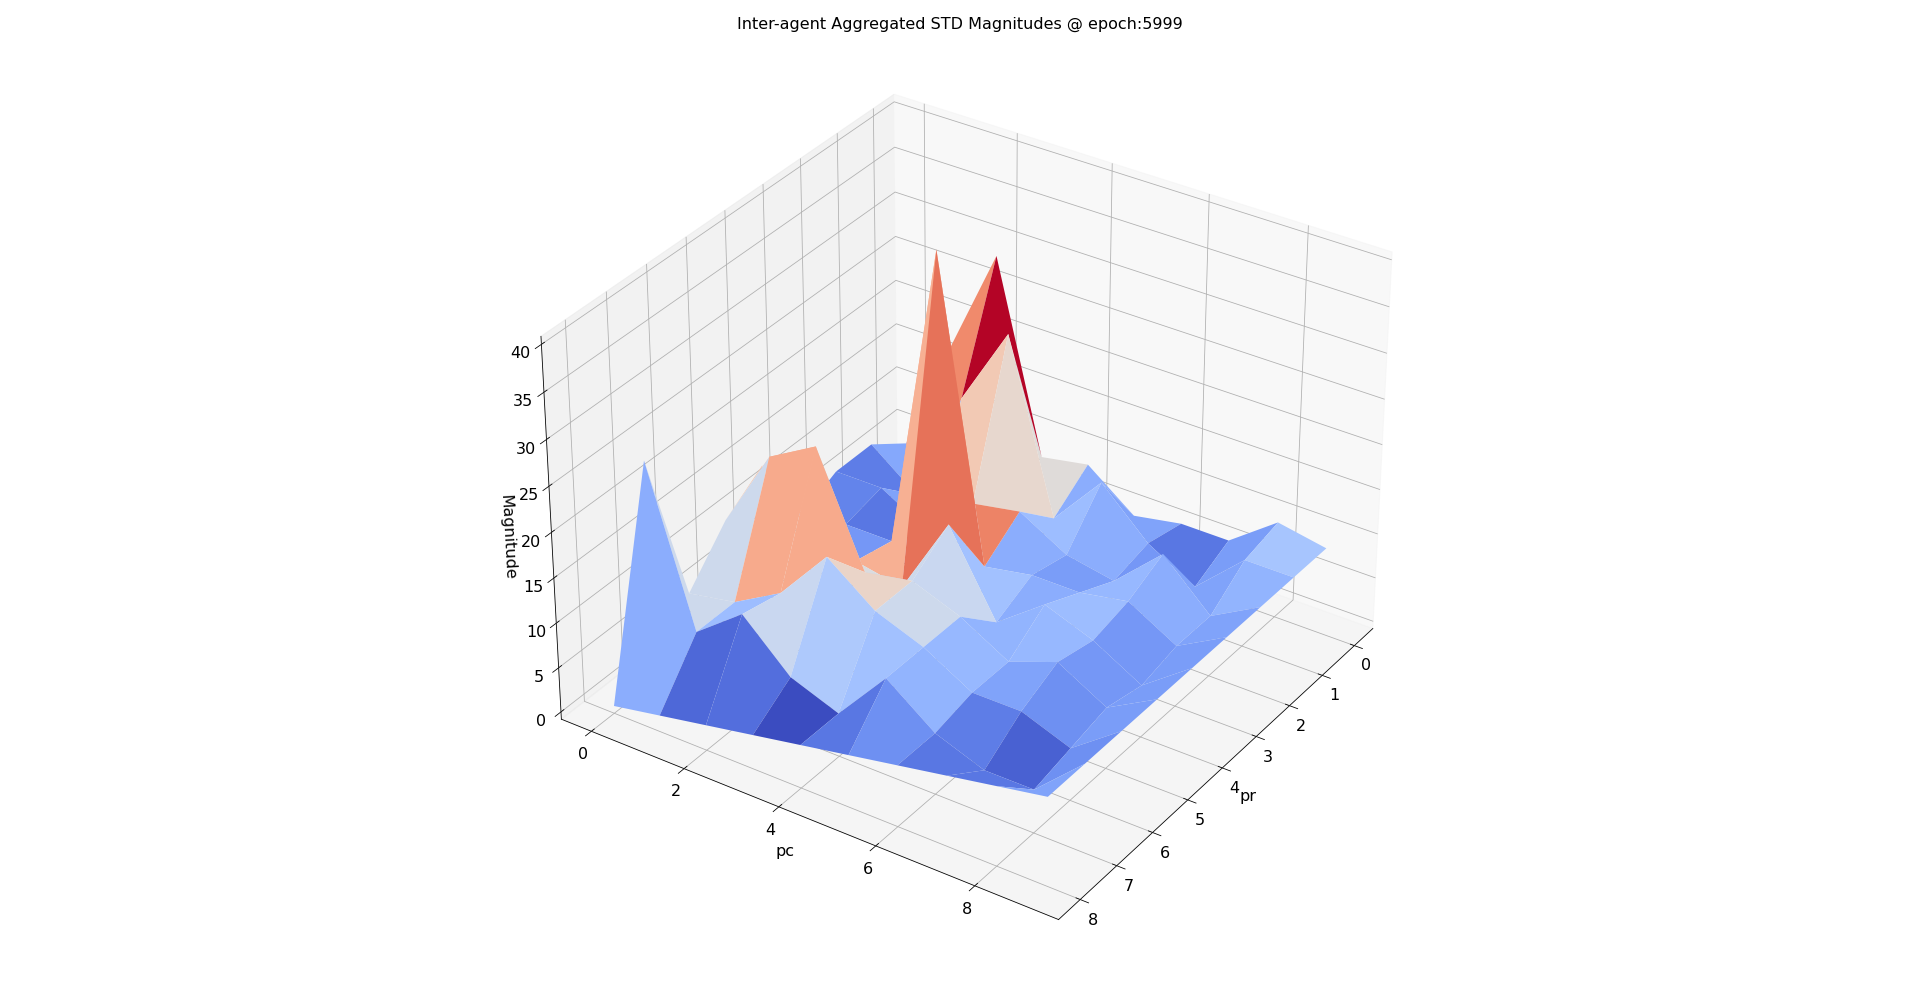
\includegraphics[width=8cm]{figures/Experiment3}
	\end{center}
	\caption{Experiment End \label{fig:experiment3}}
\end{figure}

The first area of comparison is the effect of the algorithms on the number of perimeter agents. The baseline swarm's agents oscillates but remain in a relatively stable state with a constant number of perimeter agents and the internal anomaly persists~(Fig.~\ref{fig:baselineSwarm}). The maximum and minimum number of perimeter agents is shown in table~\ref{tab:perimeterLimits}. 

\begin{figure}[H]
	\begin{center}
		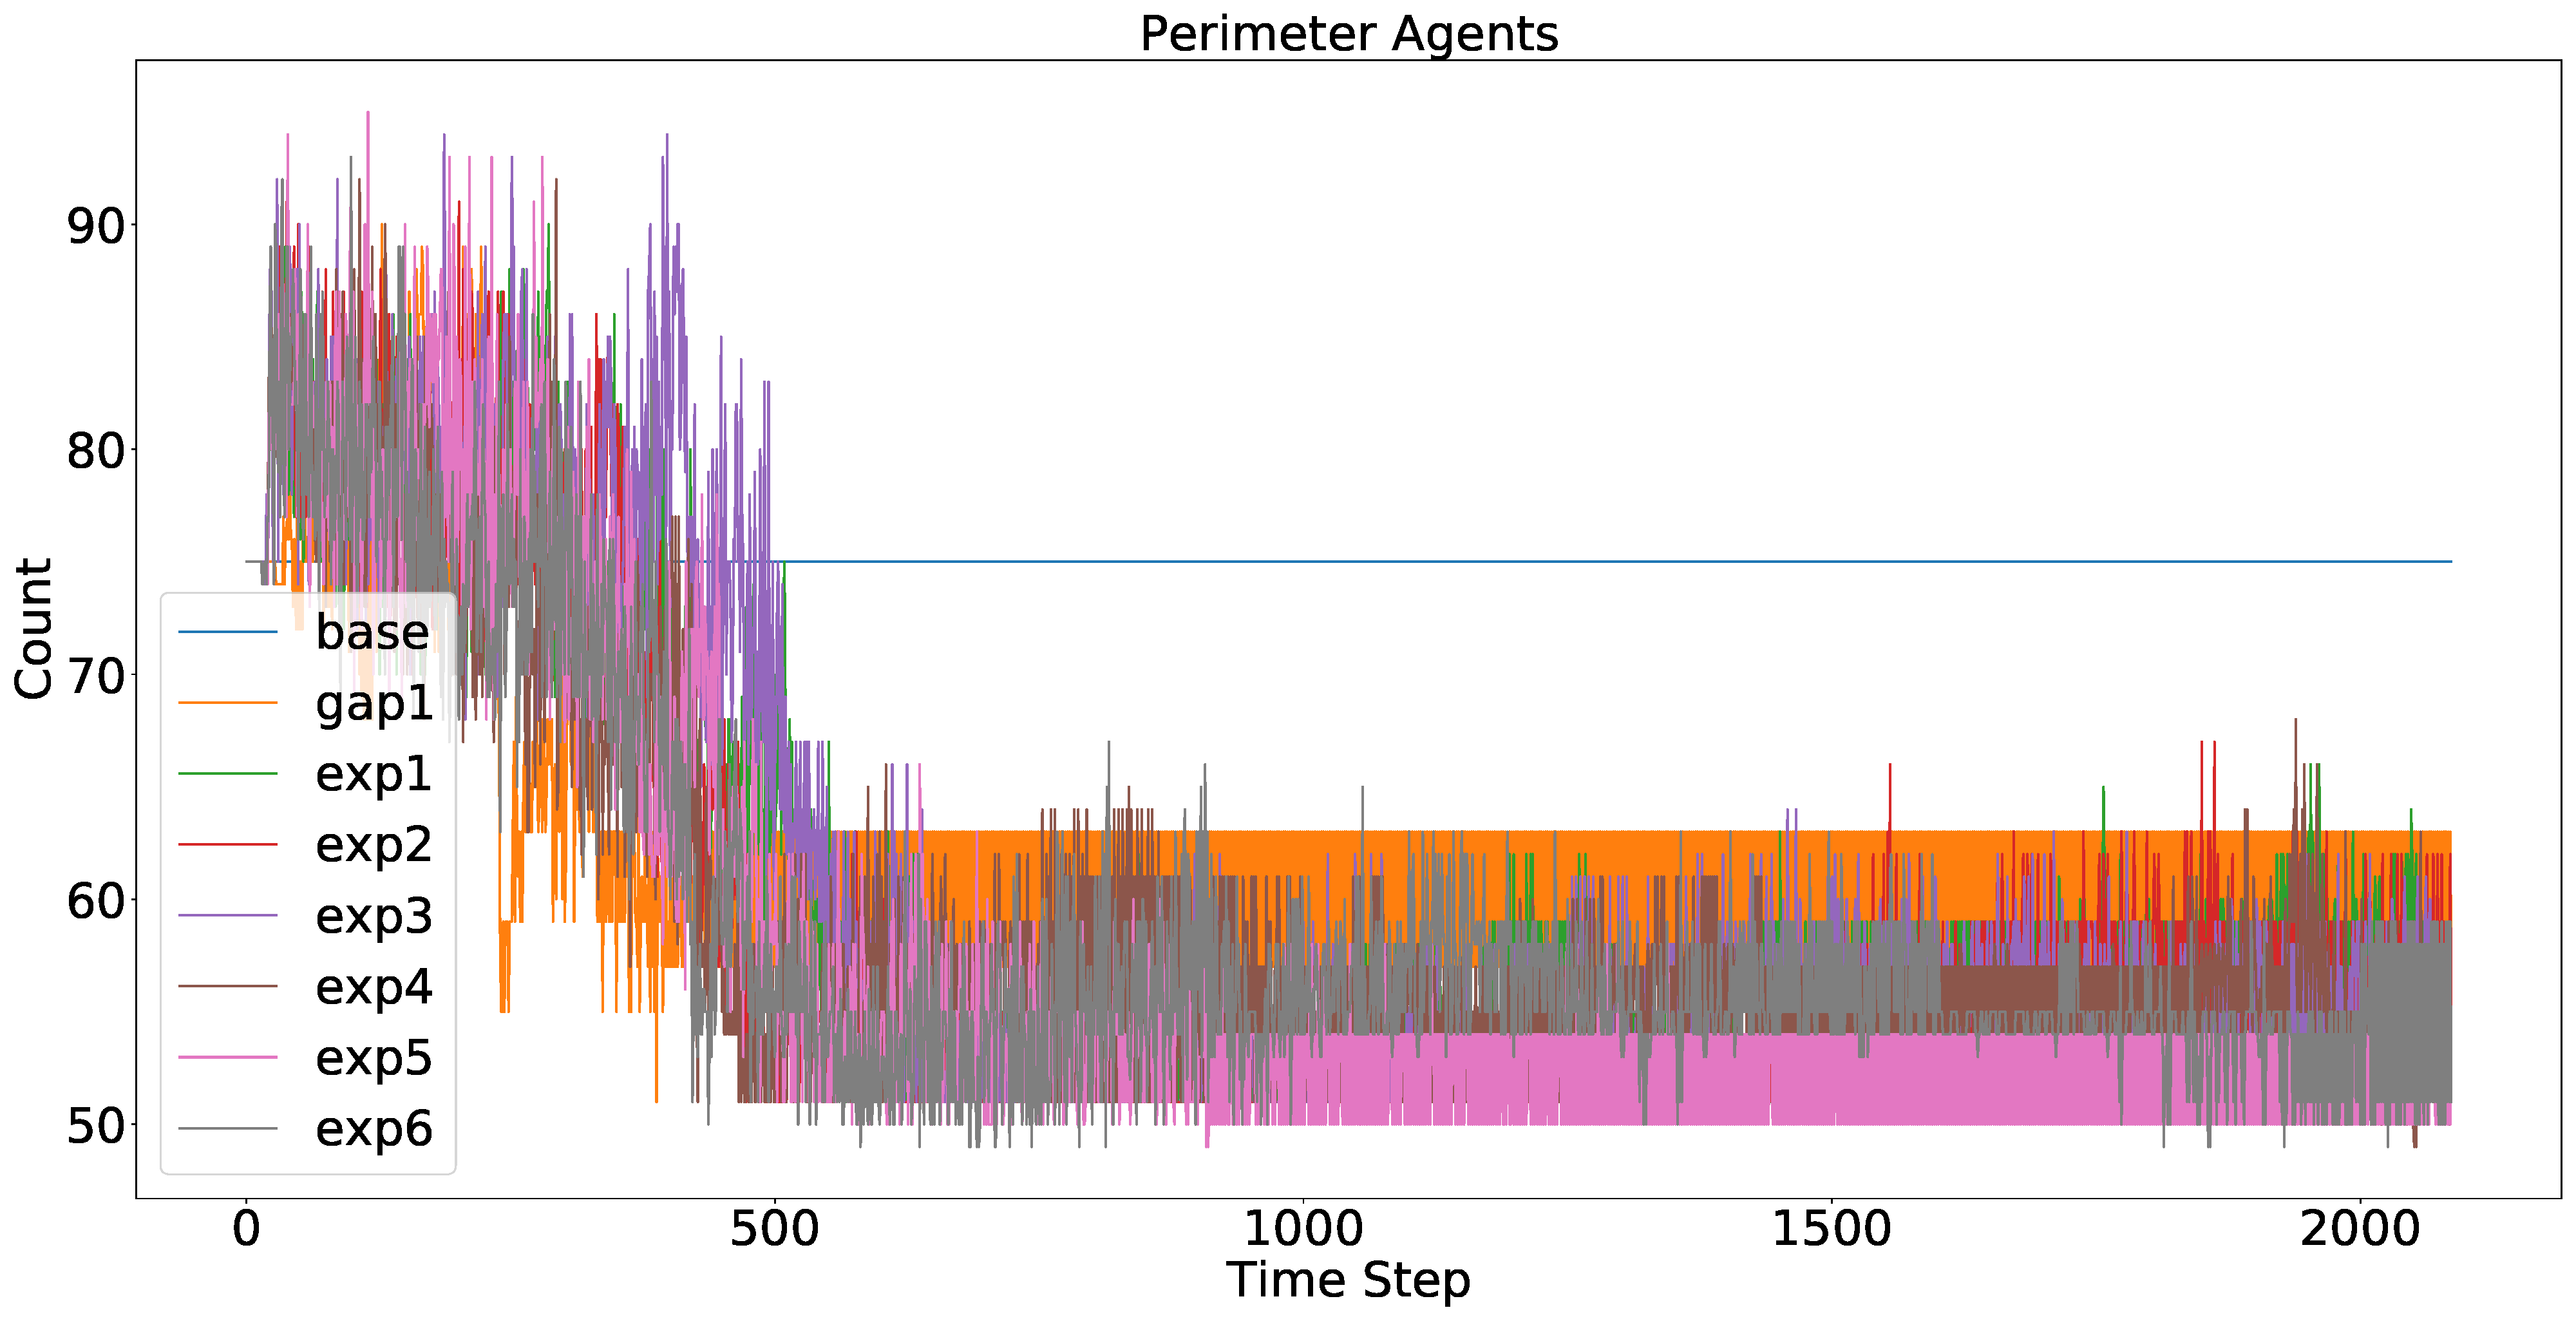
\includegraphics[width=8cm]{figures/PerimeterCount}
	\end{center}
	\caption{Perimeter Count of baseline, gap reduction and perimeter compression. \label{fig:perimeterCount}}
\end{figure}

\begin{table}[ht]
	\centering
	\tiny
	\begin{tabular}{|c|c|r|r|r|r|r|r|r|}
		\hline
		\rowcolor[HTML]{000000} 
		{\color[HTML]{FFFFFF} Comp.} &{\color[HTML]{FFFFFF} Base} & {\color[HTML]{FFFFFF} Void} & {\color[HTML]{FFFFFF} 1} & {\color[HTML]{FFFFFF} 2} & {\color[HTML]{FFFFFF} 3} & {\color[HTML]{FFFFFF} 4} & {\color[HTML]{FFFFFF} 5} & {\color[HTML]{FFFFFF} 6}\\ \hline
		Max & \texttt{75} & \texttt{90} &\texttt{90} & \texttt{90} & \texttt{94} & \texttt{92} & \texttt{95} & \texttt{93} \\ \hline
		Min & \texttt{75} & \texttt{51} &\texttt{51}  & \texttt{51} & \texttt{51} & \texttt{49} & \texttt{49} & \texttt{49}\\ \hline
		Mean & \texttt{75} & \texttt{62} &\texttt{59}  & \texttt{58} & \texttt{60} & \texttt{59} & \texttt{57} & \texttt{59}\\ \hline
		Std & \texttt{0} & \texttt{6} &\texttt{9}  & \texttt{10} & \texttt{10} & \texttt{8} & \texttt{10} & \texttt{8}\\ \hline
	\end{tabular}
	\caption{Perimeter agents}
	\label{tab:perimeterLimits}
\end{table}

\begin{figure}[H]
	\begin{center}
		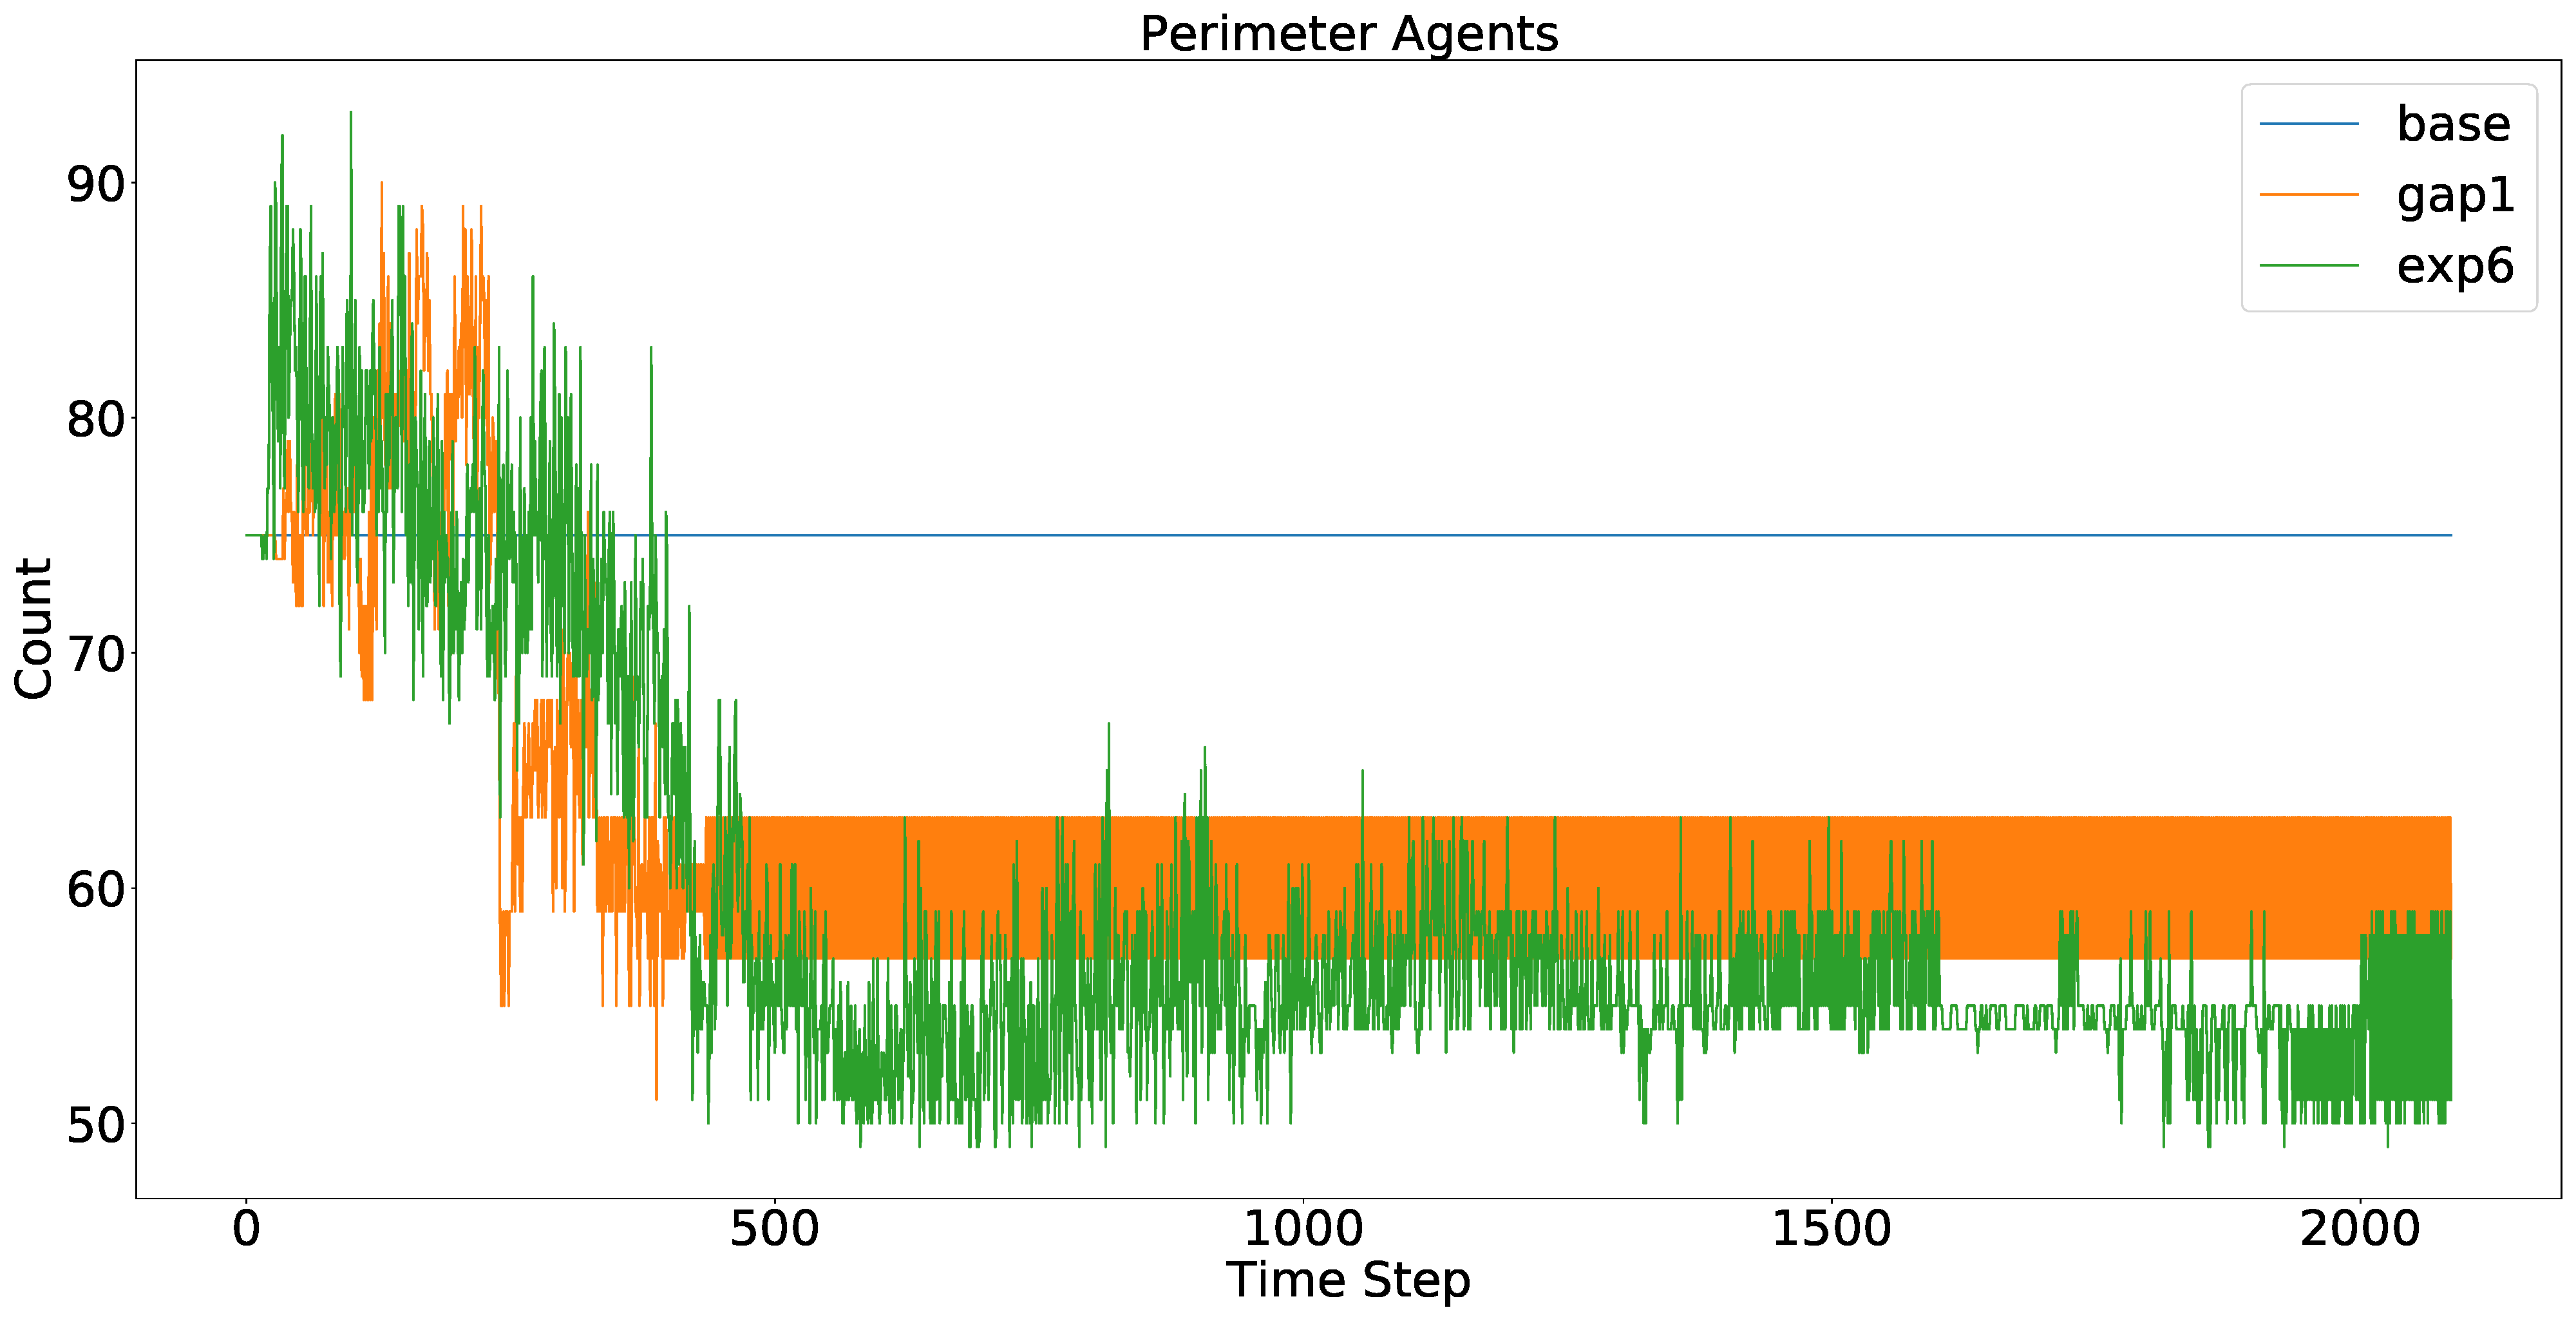
\includegraphics[width=8cm]{figures/PerimeterCount2}
	\end{center}
	\caption{Perimeter Count of baseline, gap reduction and Experiment 6. \label{fig:perimeterCount2}}
\end{figure}

\begin{figure}[H]
	\begin{center}
		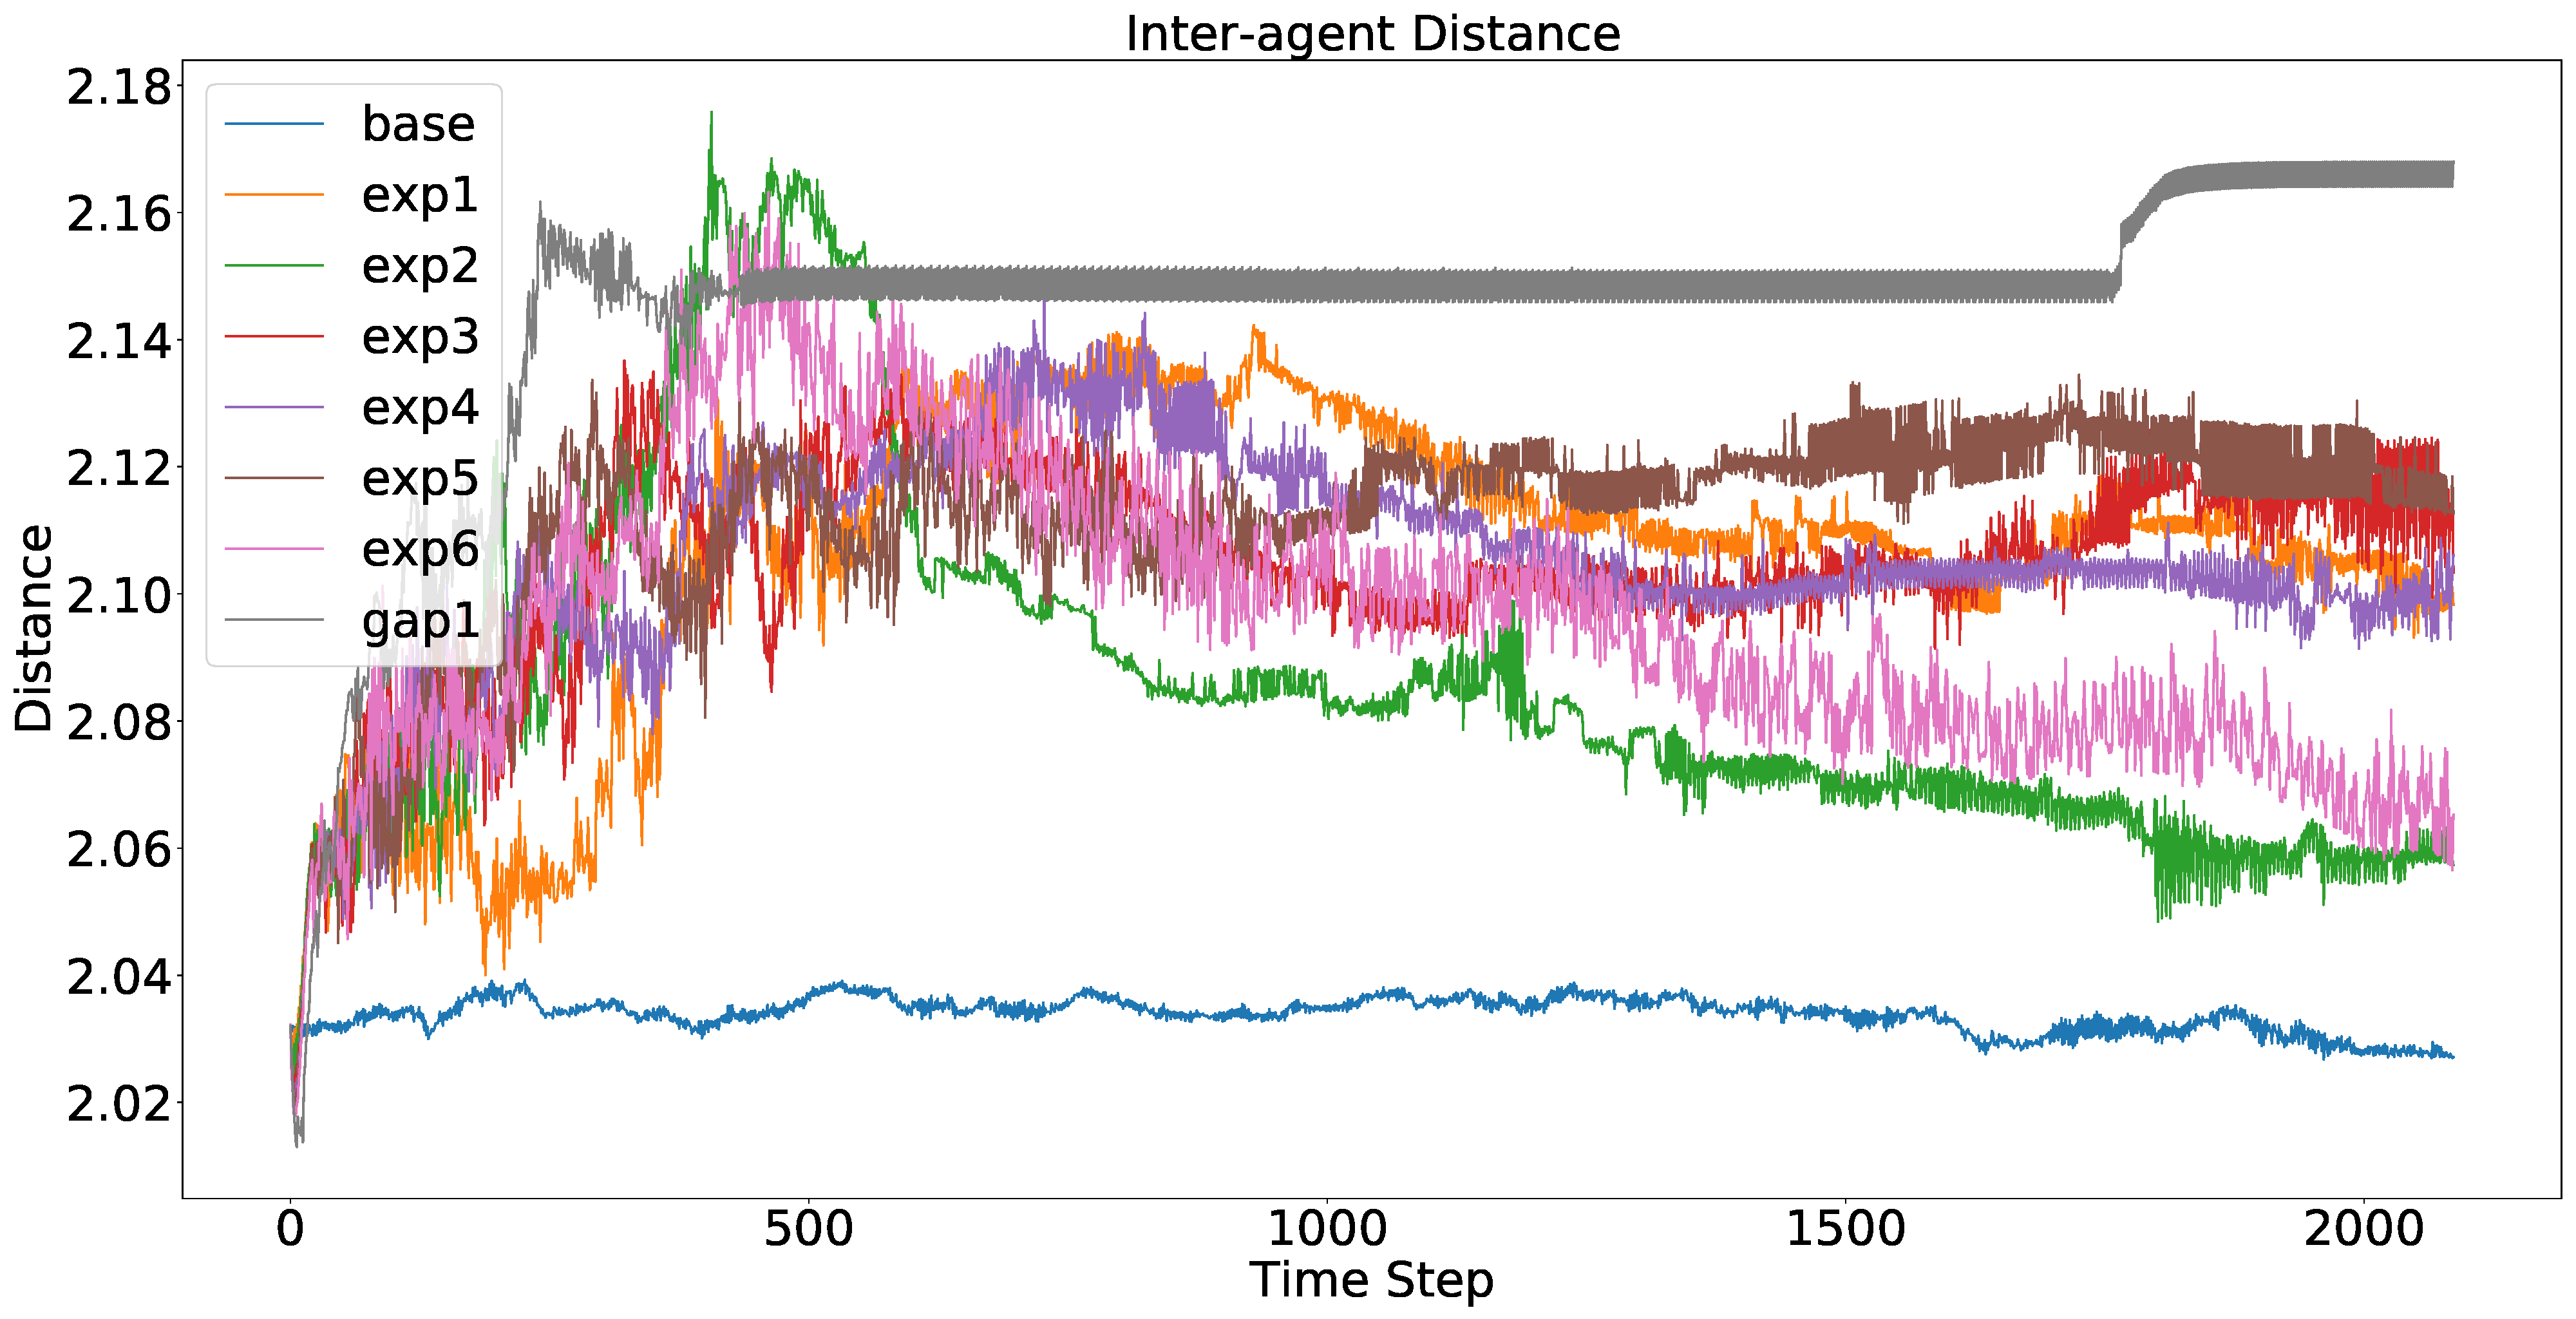
\includegraphics[width=8cm]{figures/DistanceMetric1}
	\end{center}
	\caption{Distance metric of baseline, gap reduction and perimeter compression. \label{fig:distanceMetric}}
\end{figure}

\begin{figure}[H]
	\begin{center}
		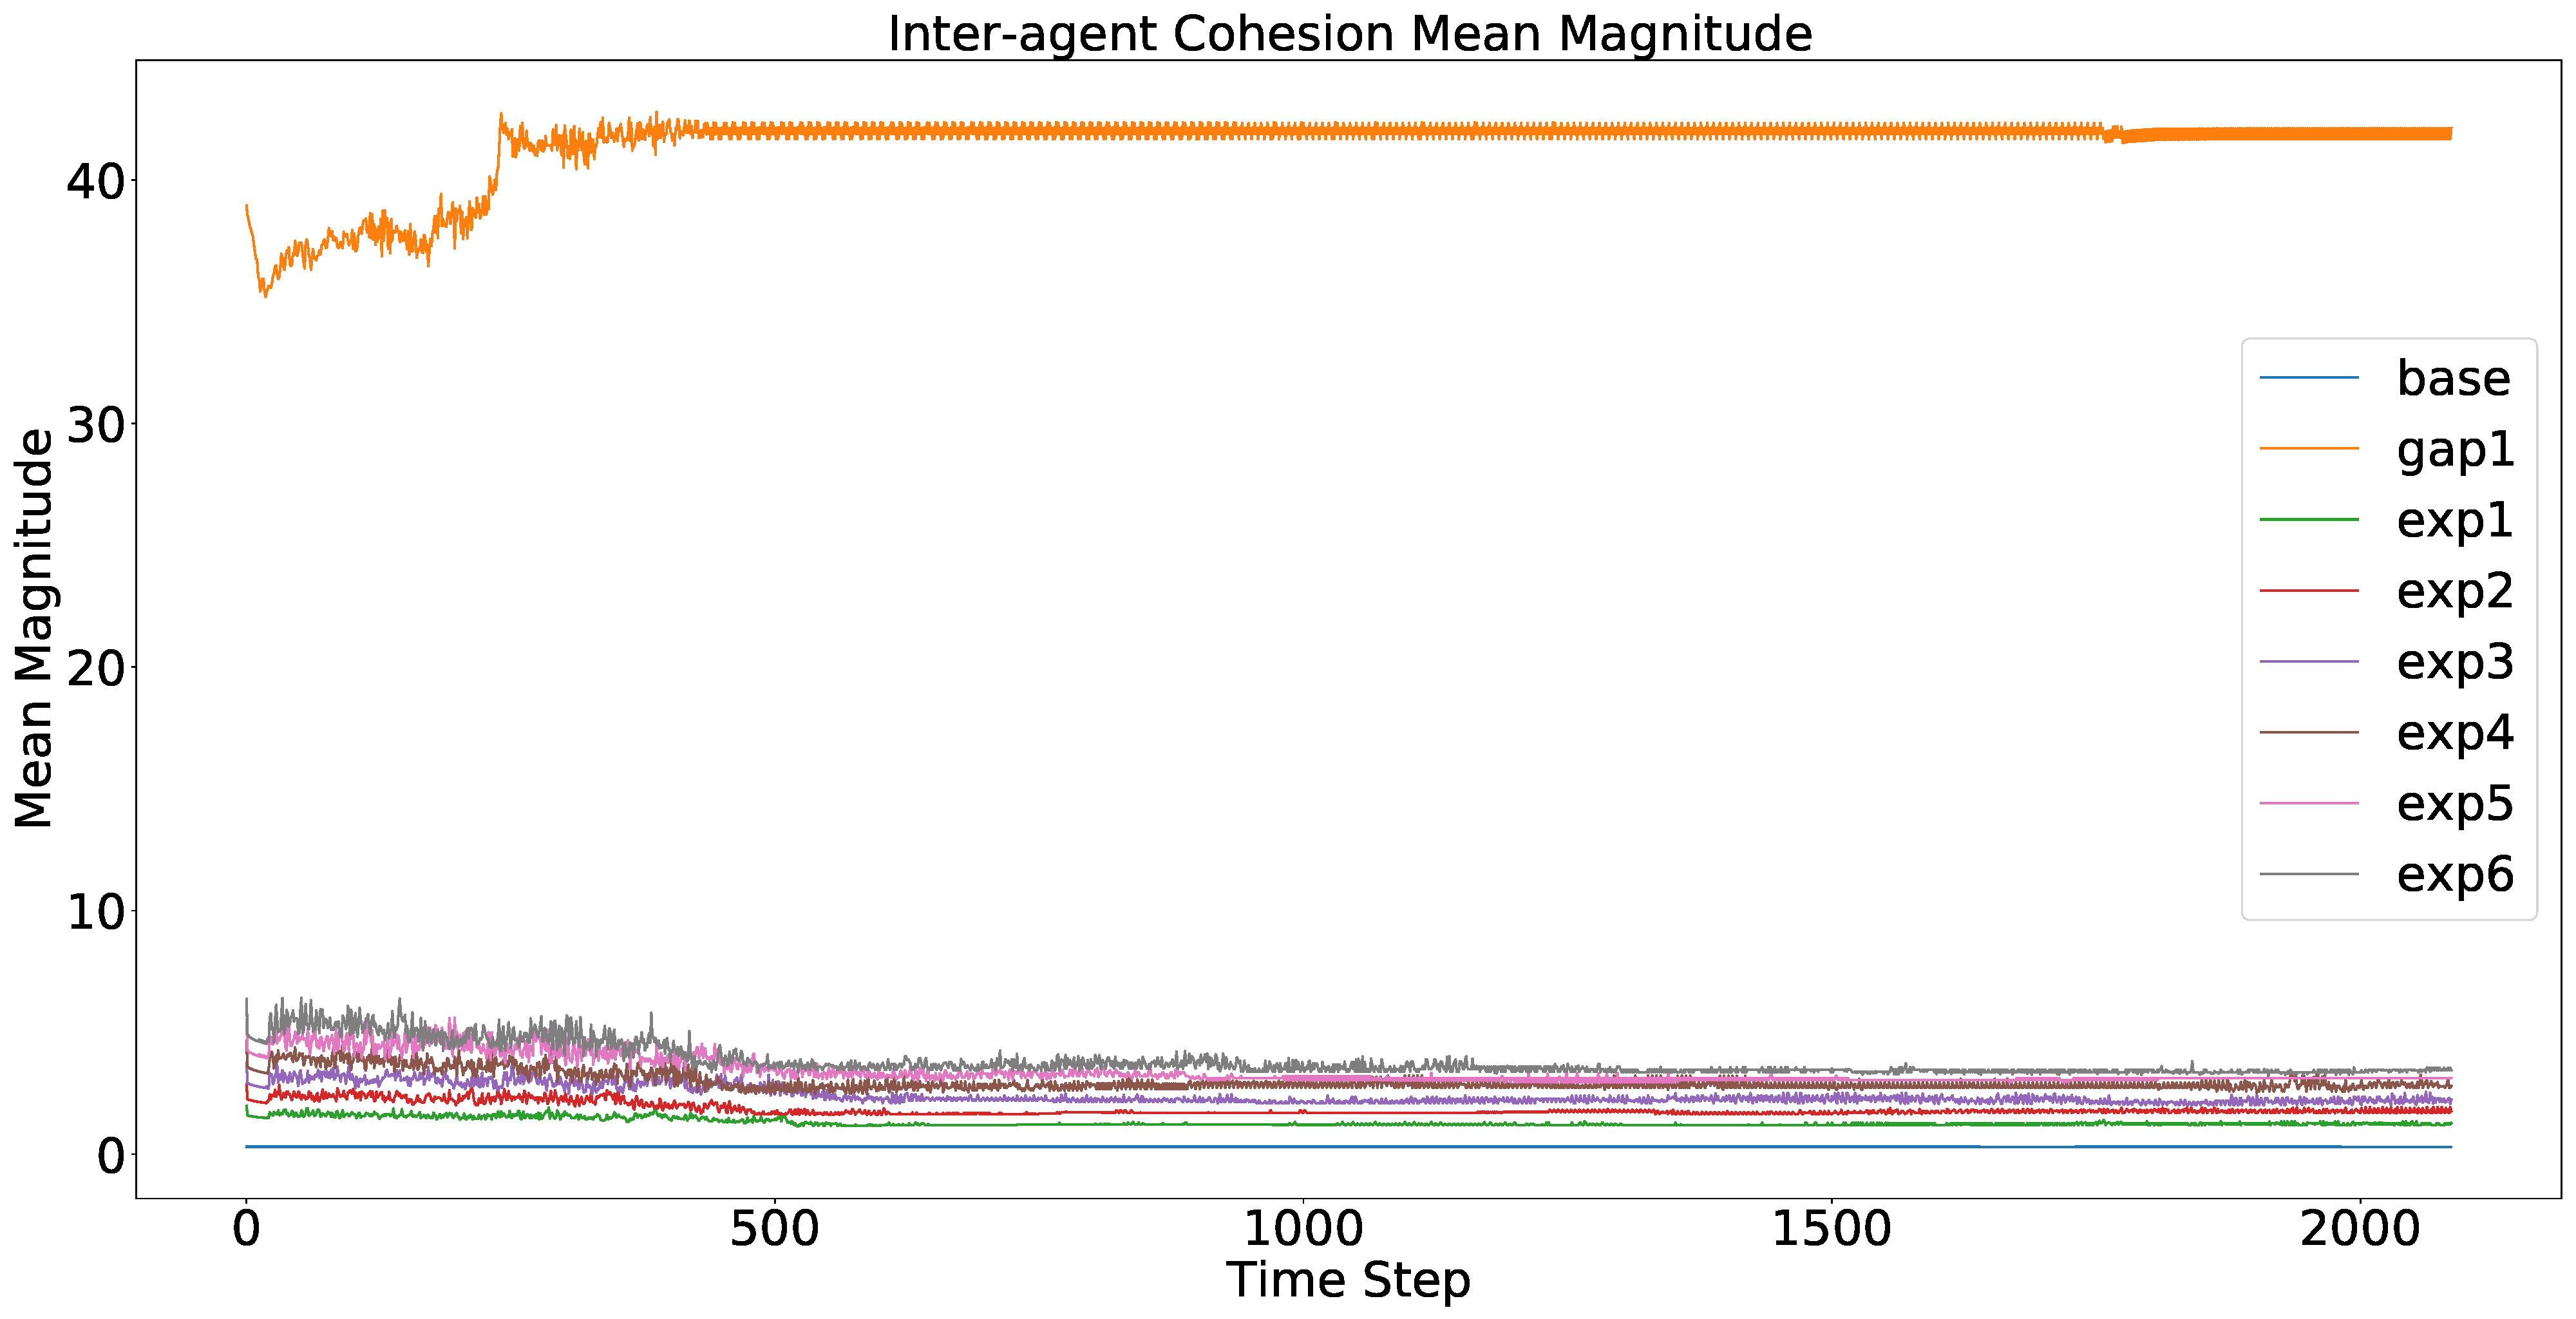
\includegraphics[width=8cm]{figures/InteragentCohesionMean}
	\end{center}
	\caption{Inter-agent Cohesion Mean. \label{fig:interagentCohesionMean}}
\end{figure}

\begin{figure}[H]
	\begin{center}
		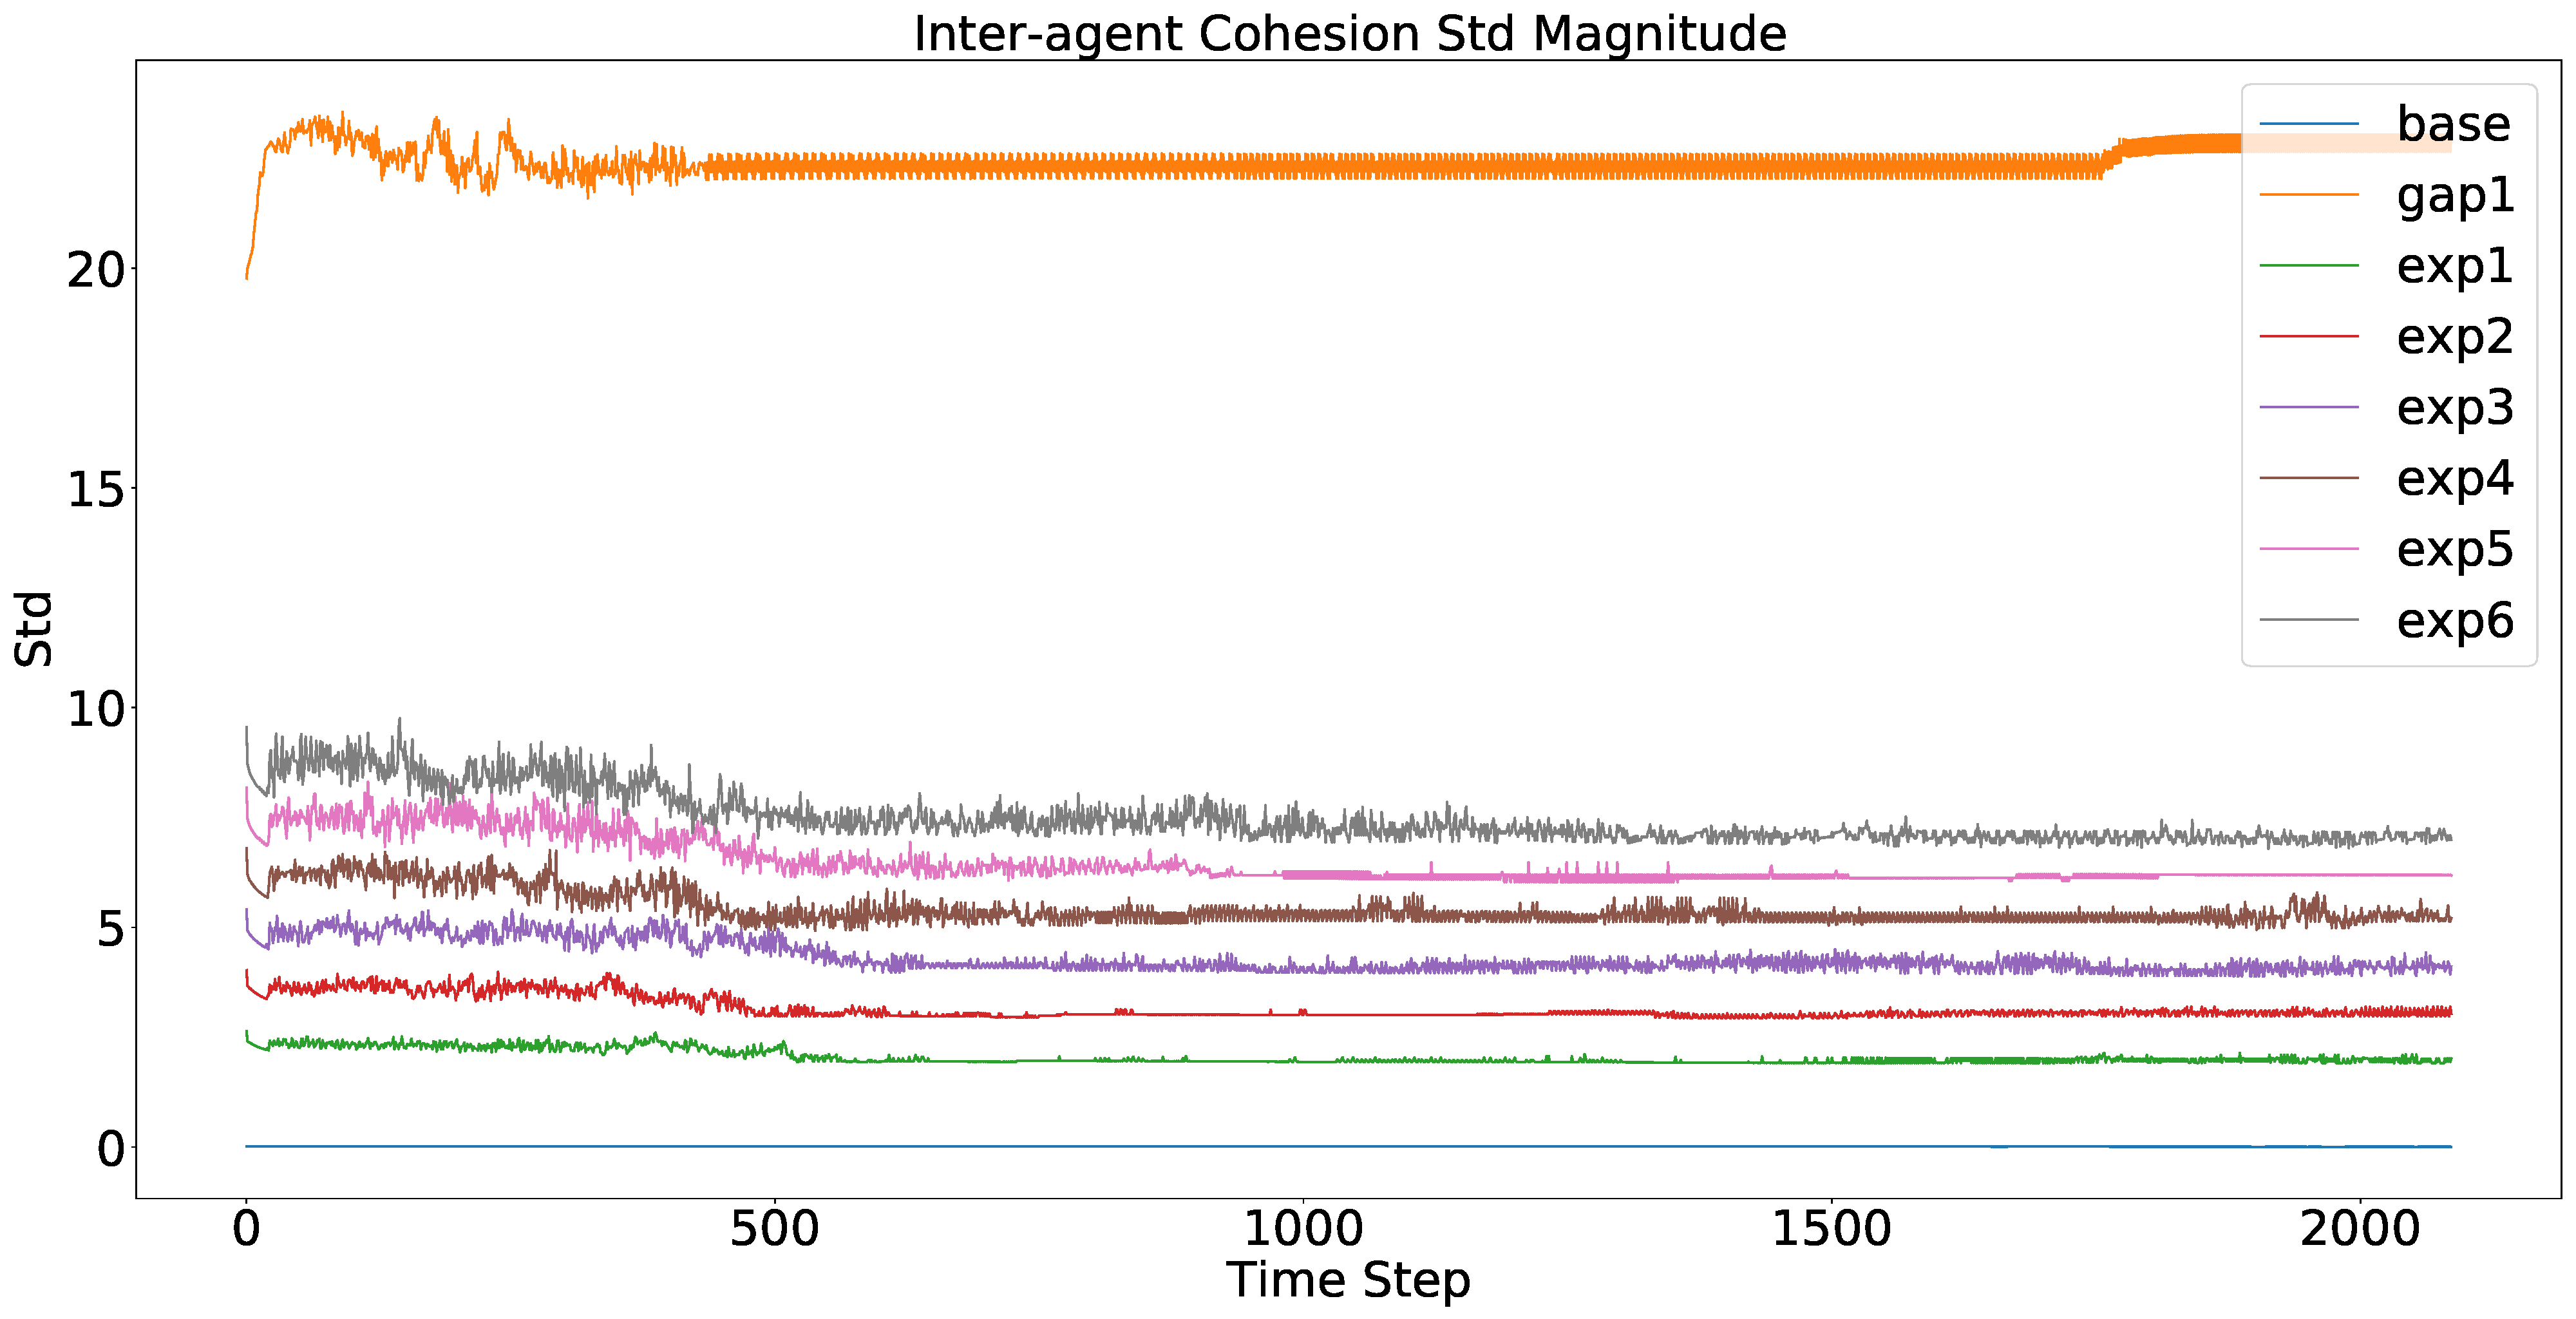
\includegraphics[width=8cm]{figures/InteragentCohesionStd}
	\end{center}
	\caption{Inter-agent Cohesion Std. \label{fig:interagentCohesionStd}}
\end{figure}

\begin{figure}[H]
	\begin{center}
		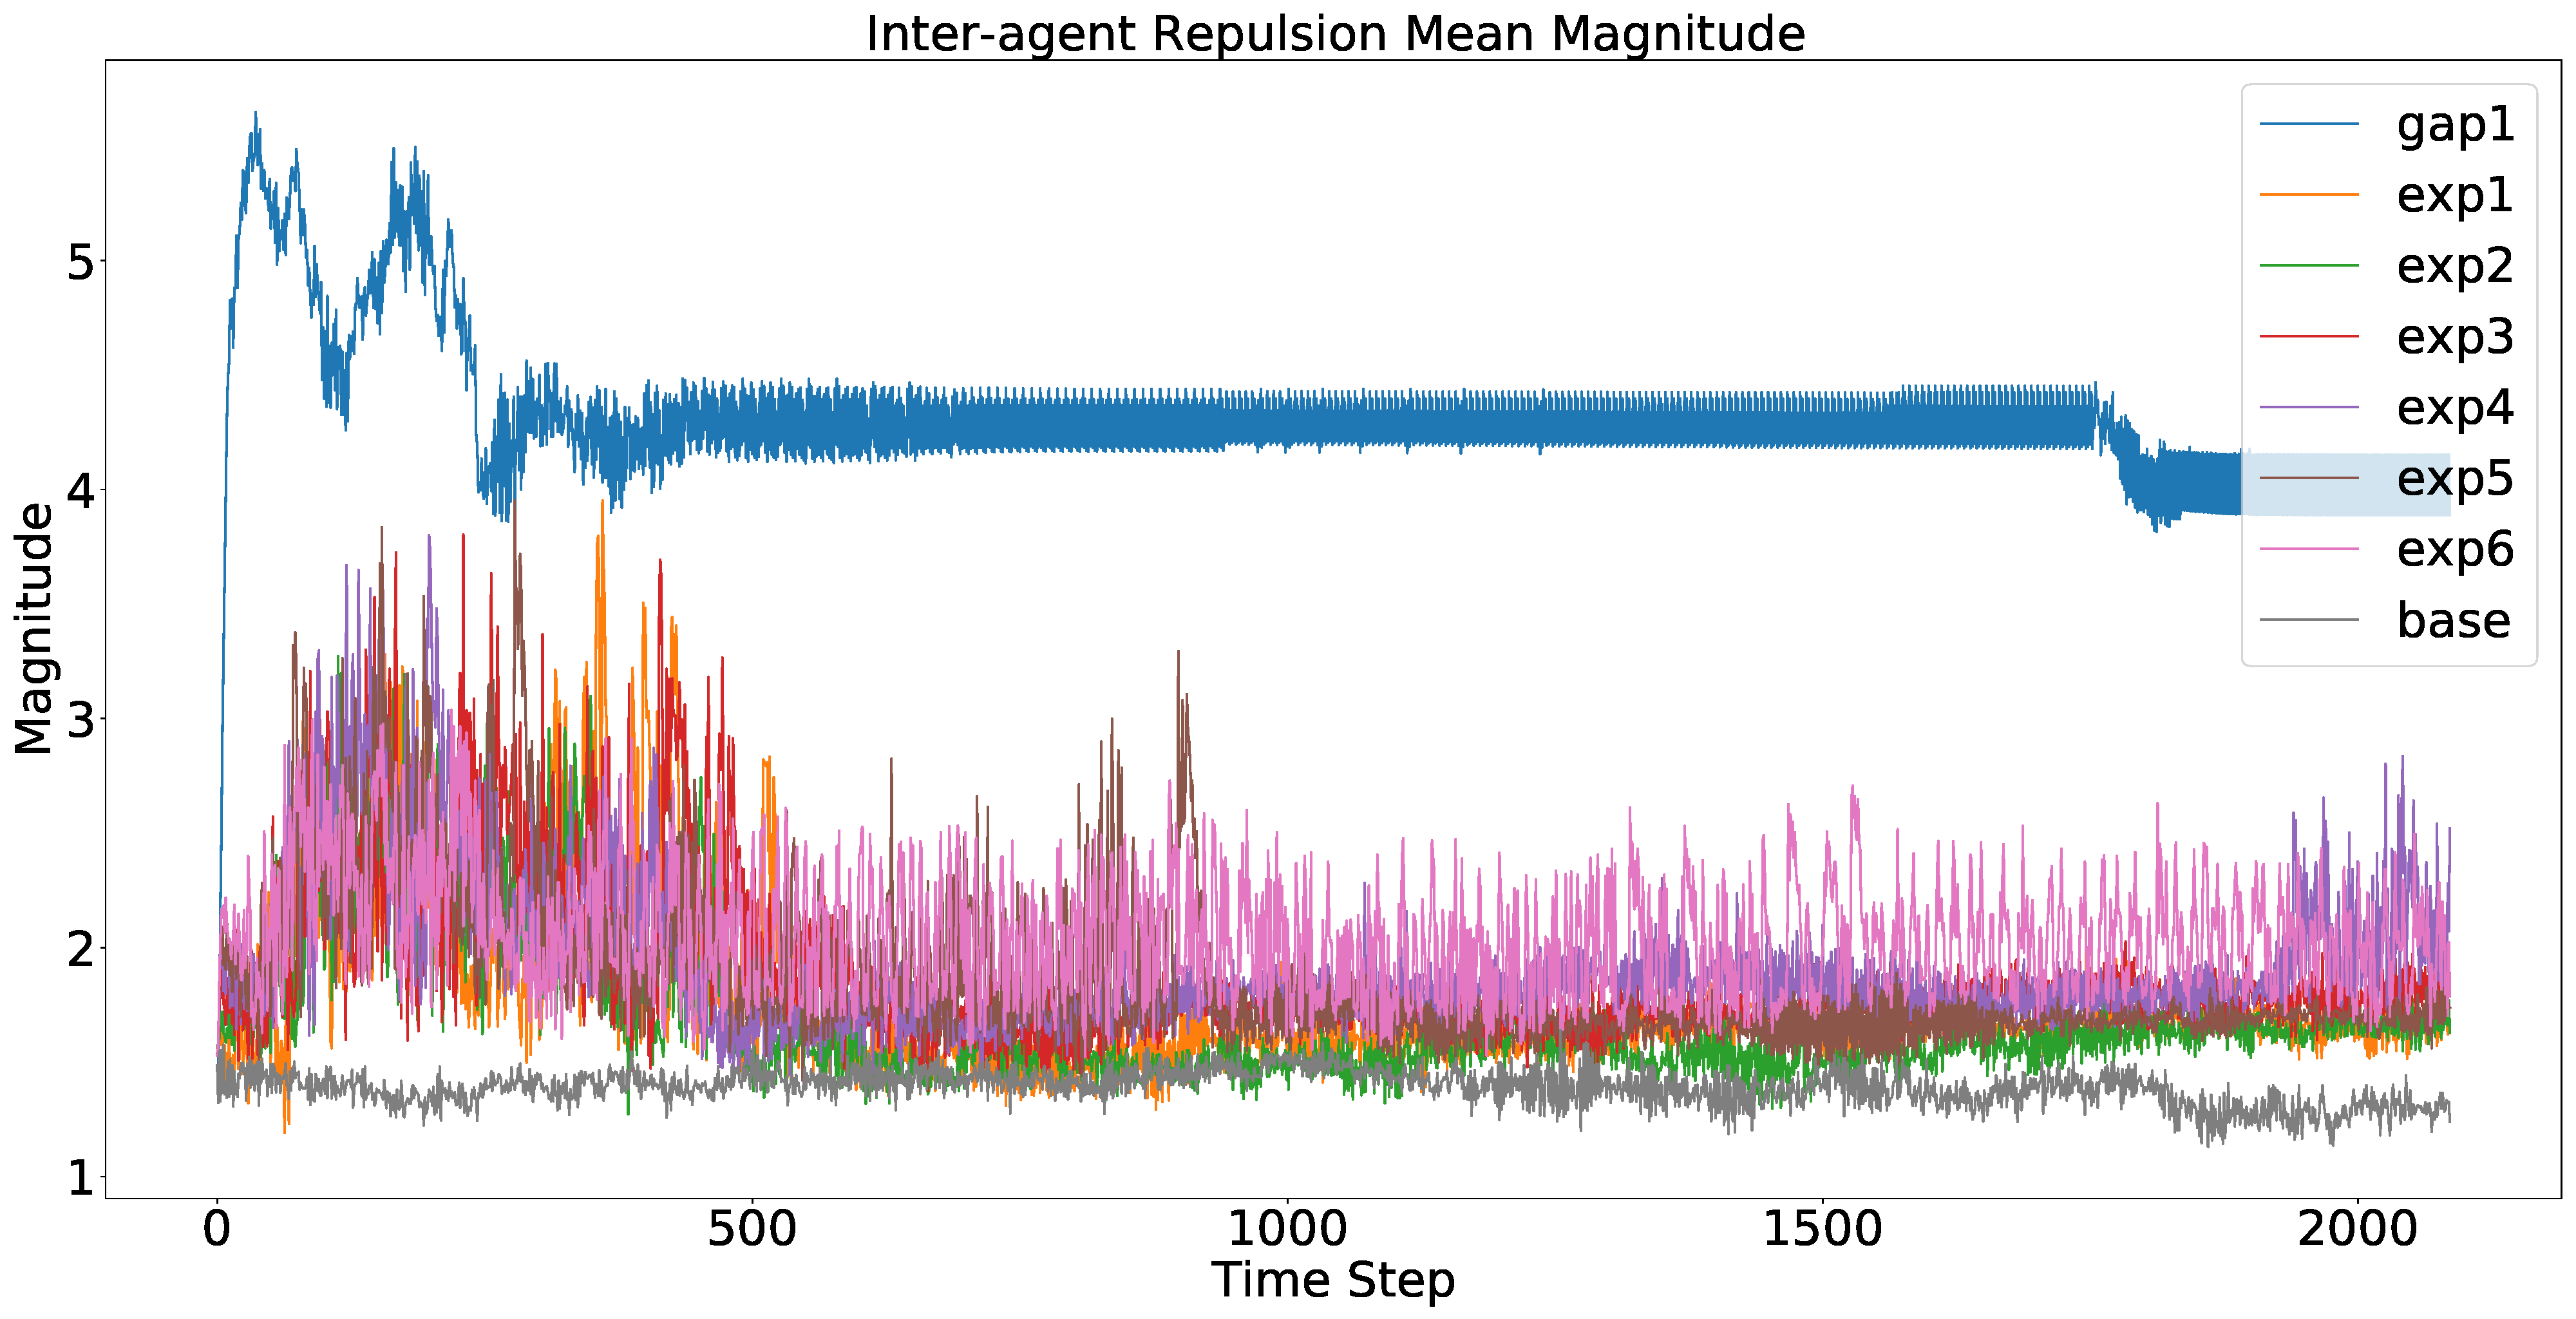
\includegraphics[width=8cm]{figures/InteragentRepulsionMean}
	\end{center}
	\caption{Inter-agent Repulsion Mean. \label{fig:interagentRepulsionMean}}
\end{figure}

\begin{figure}[H]
	\begin{center}
		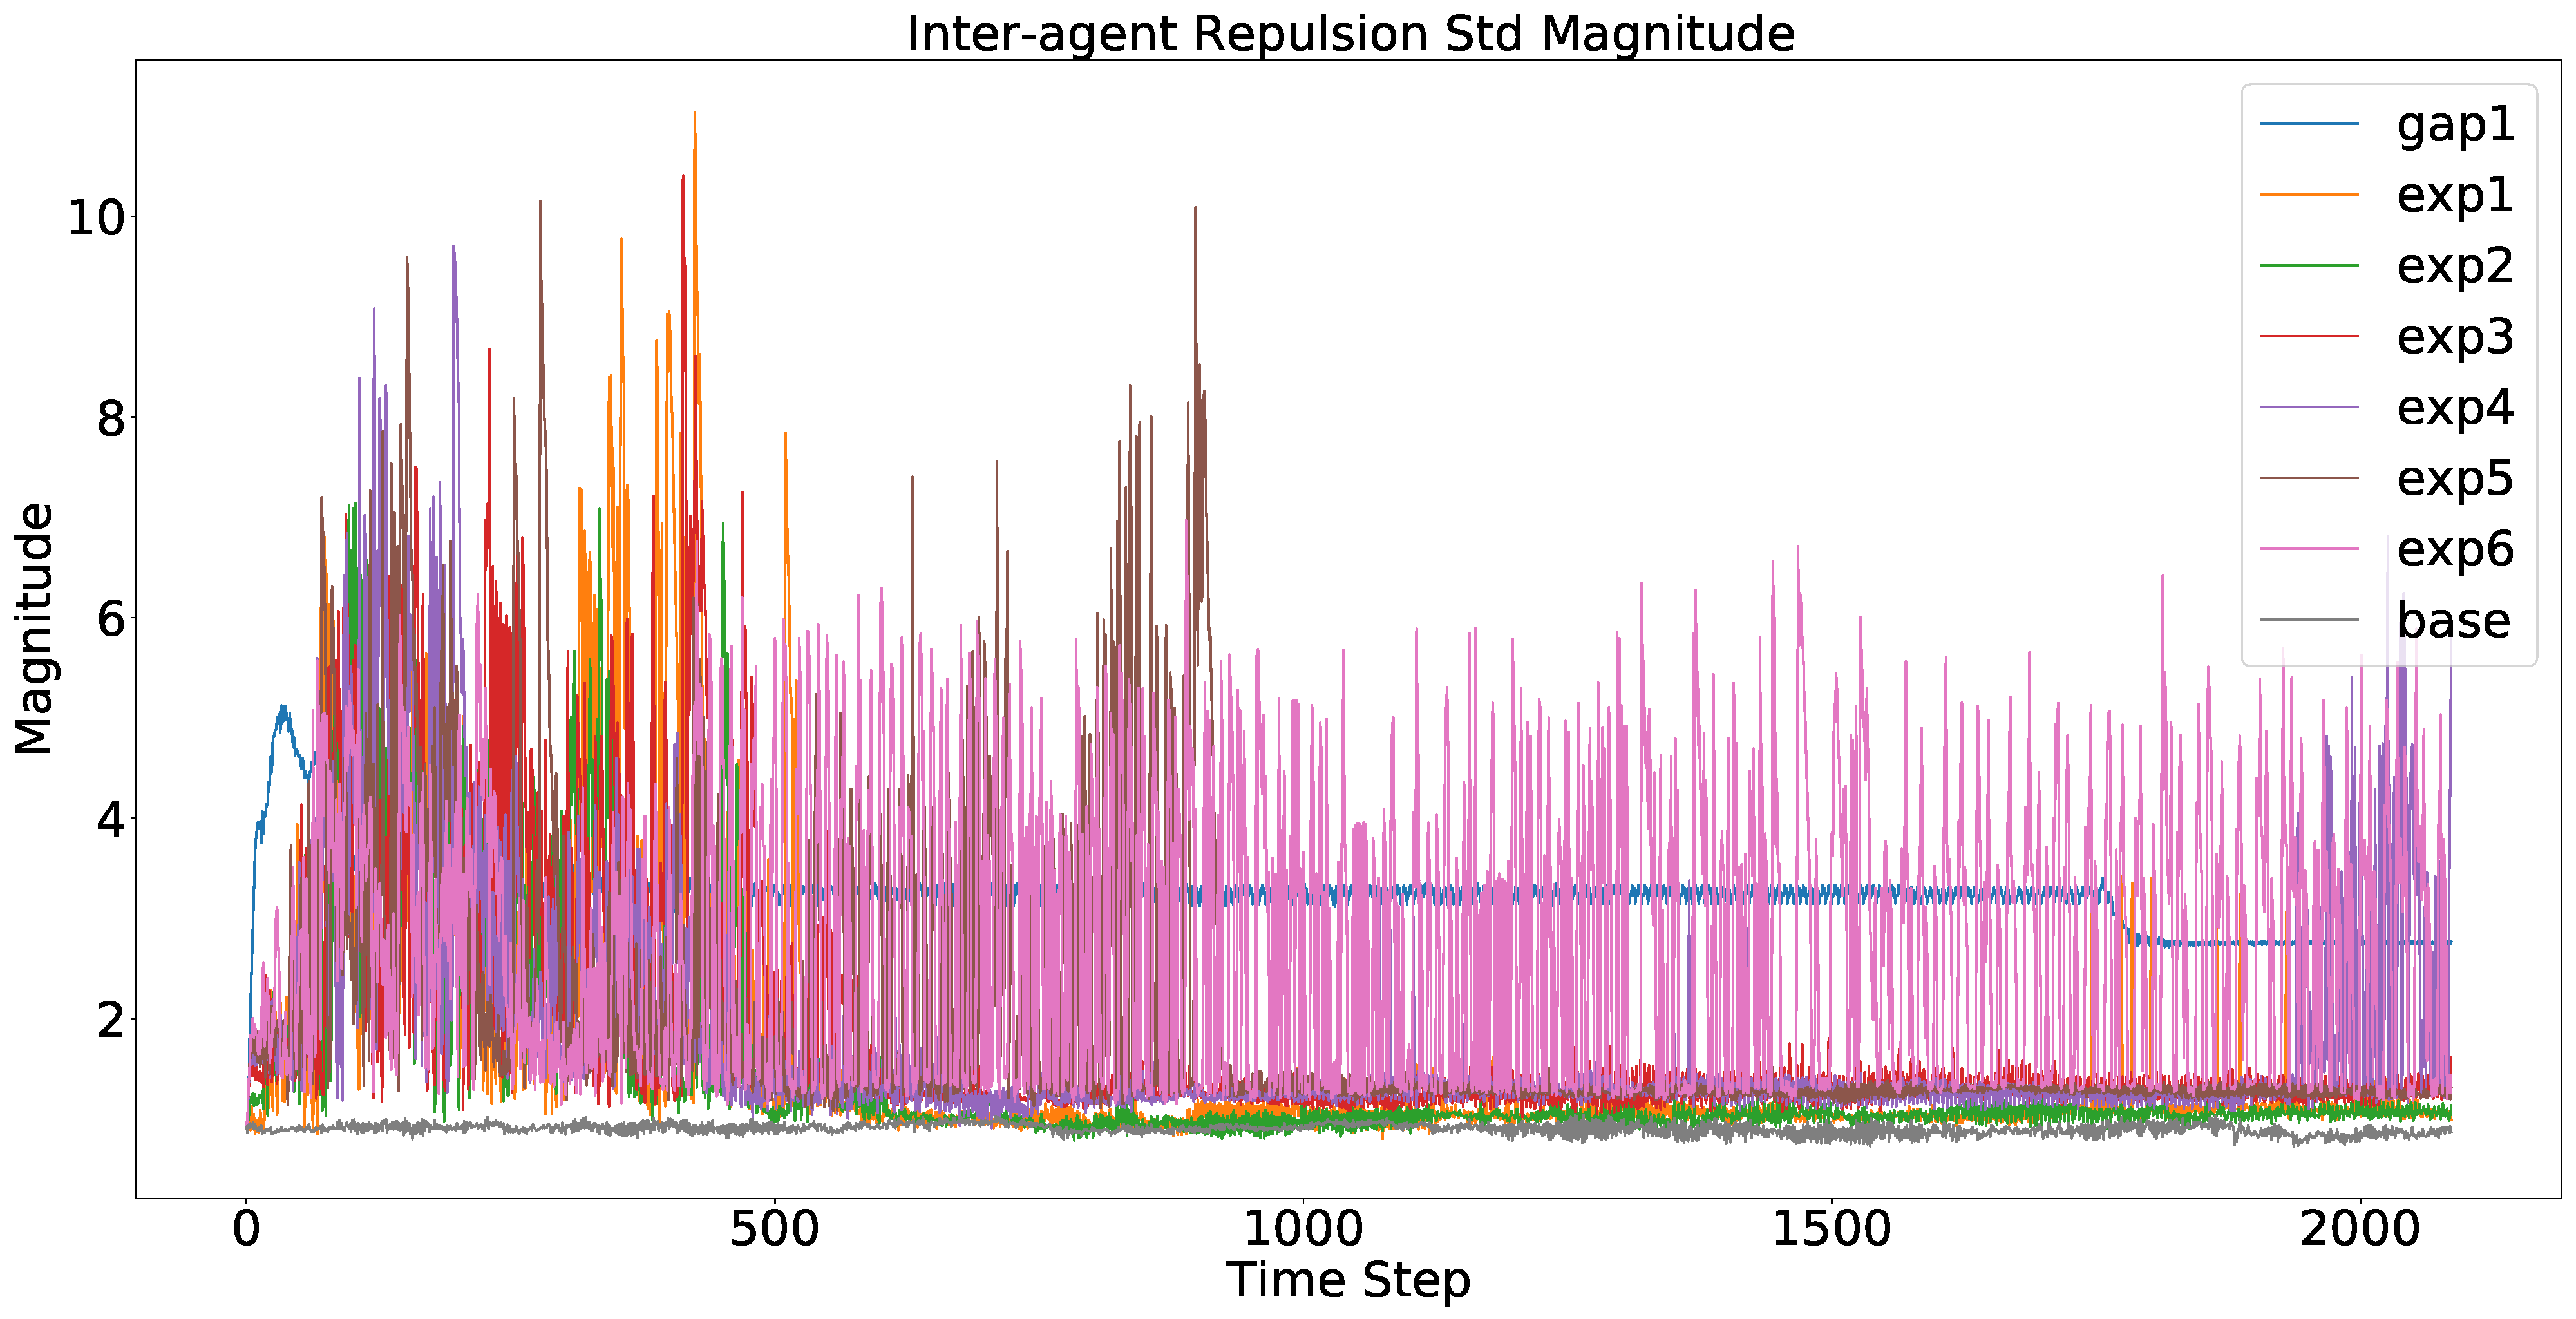
\includegraphics[width=8cm]{figures/InteragentRepulsionStd}
	\end{center}
	\caption{Inter-agent Repulsion Std. \label{fig:interagentRepulsionStd}}
\end{figure}


\begin{figure}[H]
	\begin{center}
		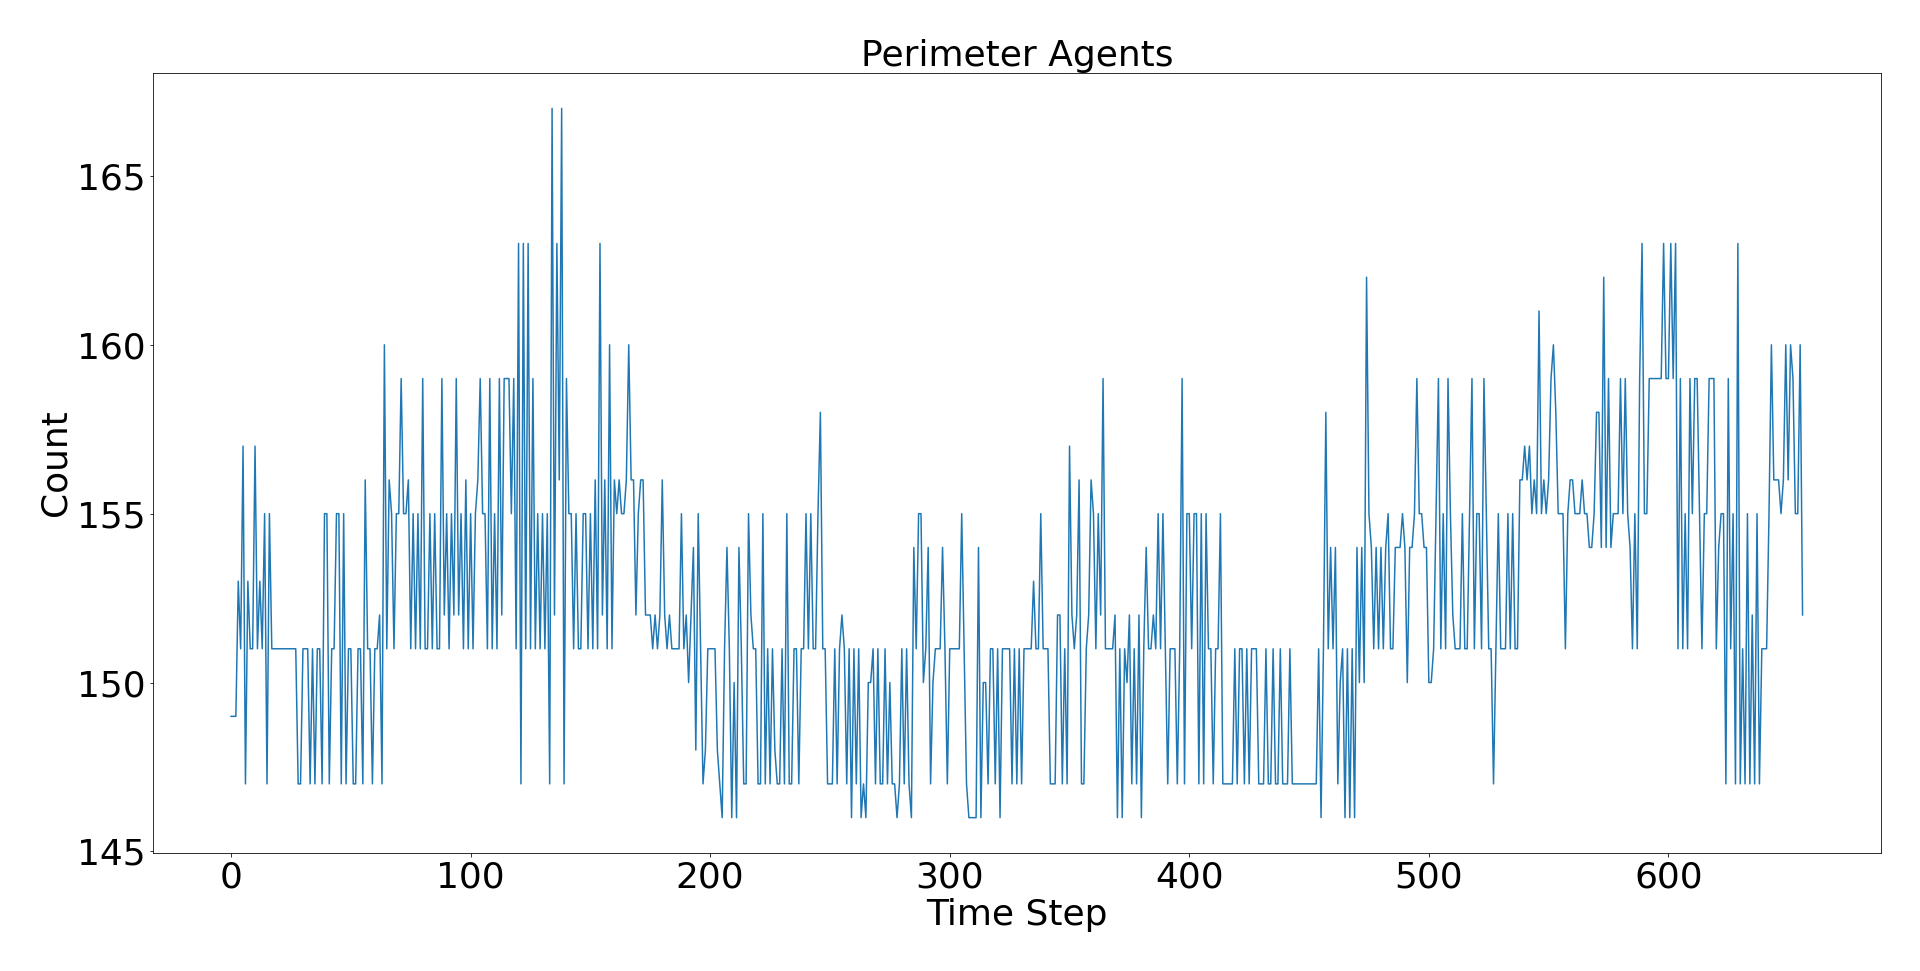
\includegraphics[width=8cm]{figures/baselineSwarmPerimeter}
	\end{center}
	\caption{Baseline swarm in stabilised configuration. \label{fig:baselineSwarmPerimeter}}
\end{figure}

\subsection{Gap compression}
\subsection{Perimeter compression}

Compression 1

\begin{figure}[H]
	\begin{center}
		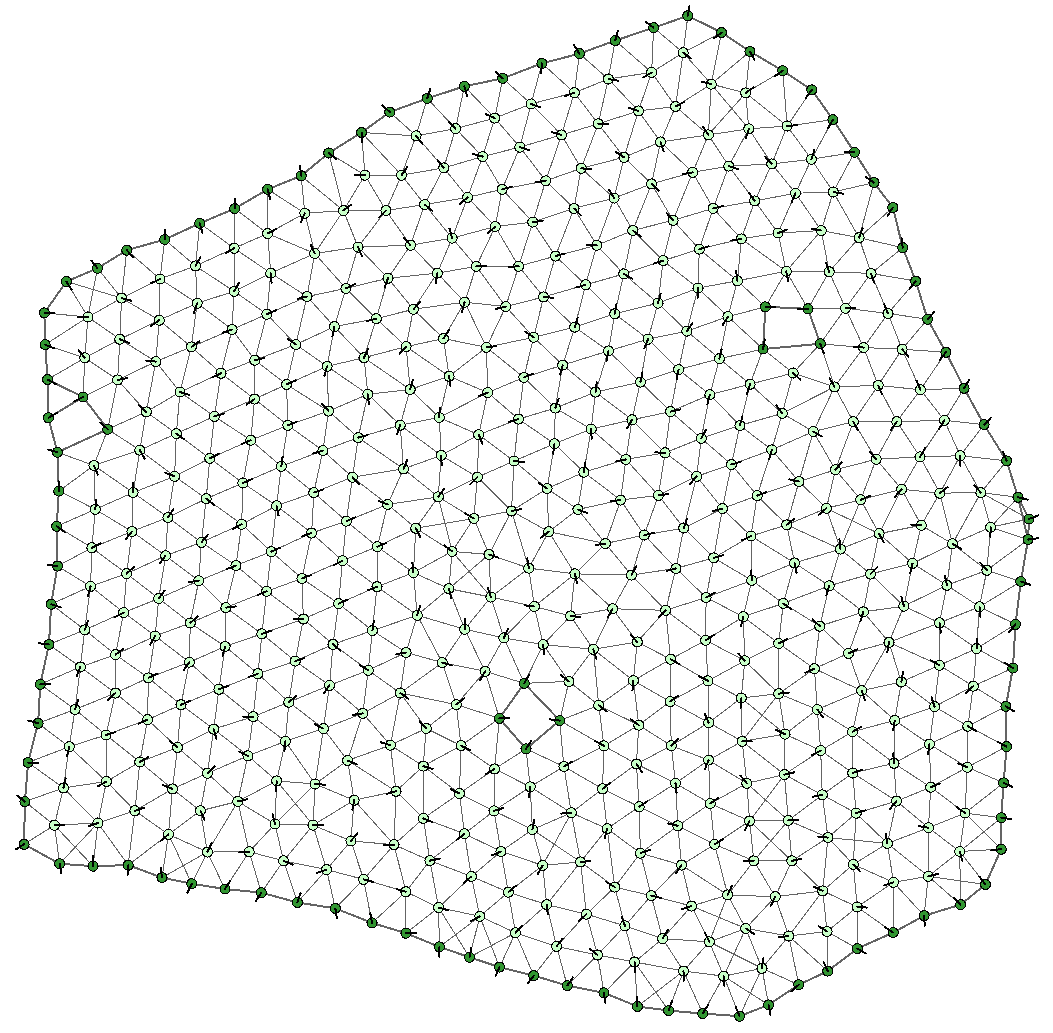
\includegraphics[width=5cm]{figures/baselineSwarm1}
	\end{center}
	\caption{Baseline swarm in with compression set 1 resultant configuration. \label{fig:baselineSwarm1}}
\end{figure}

\begin{figure}[H]
	\begin{center}
		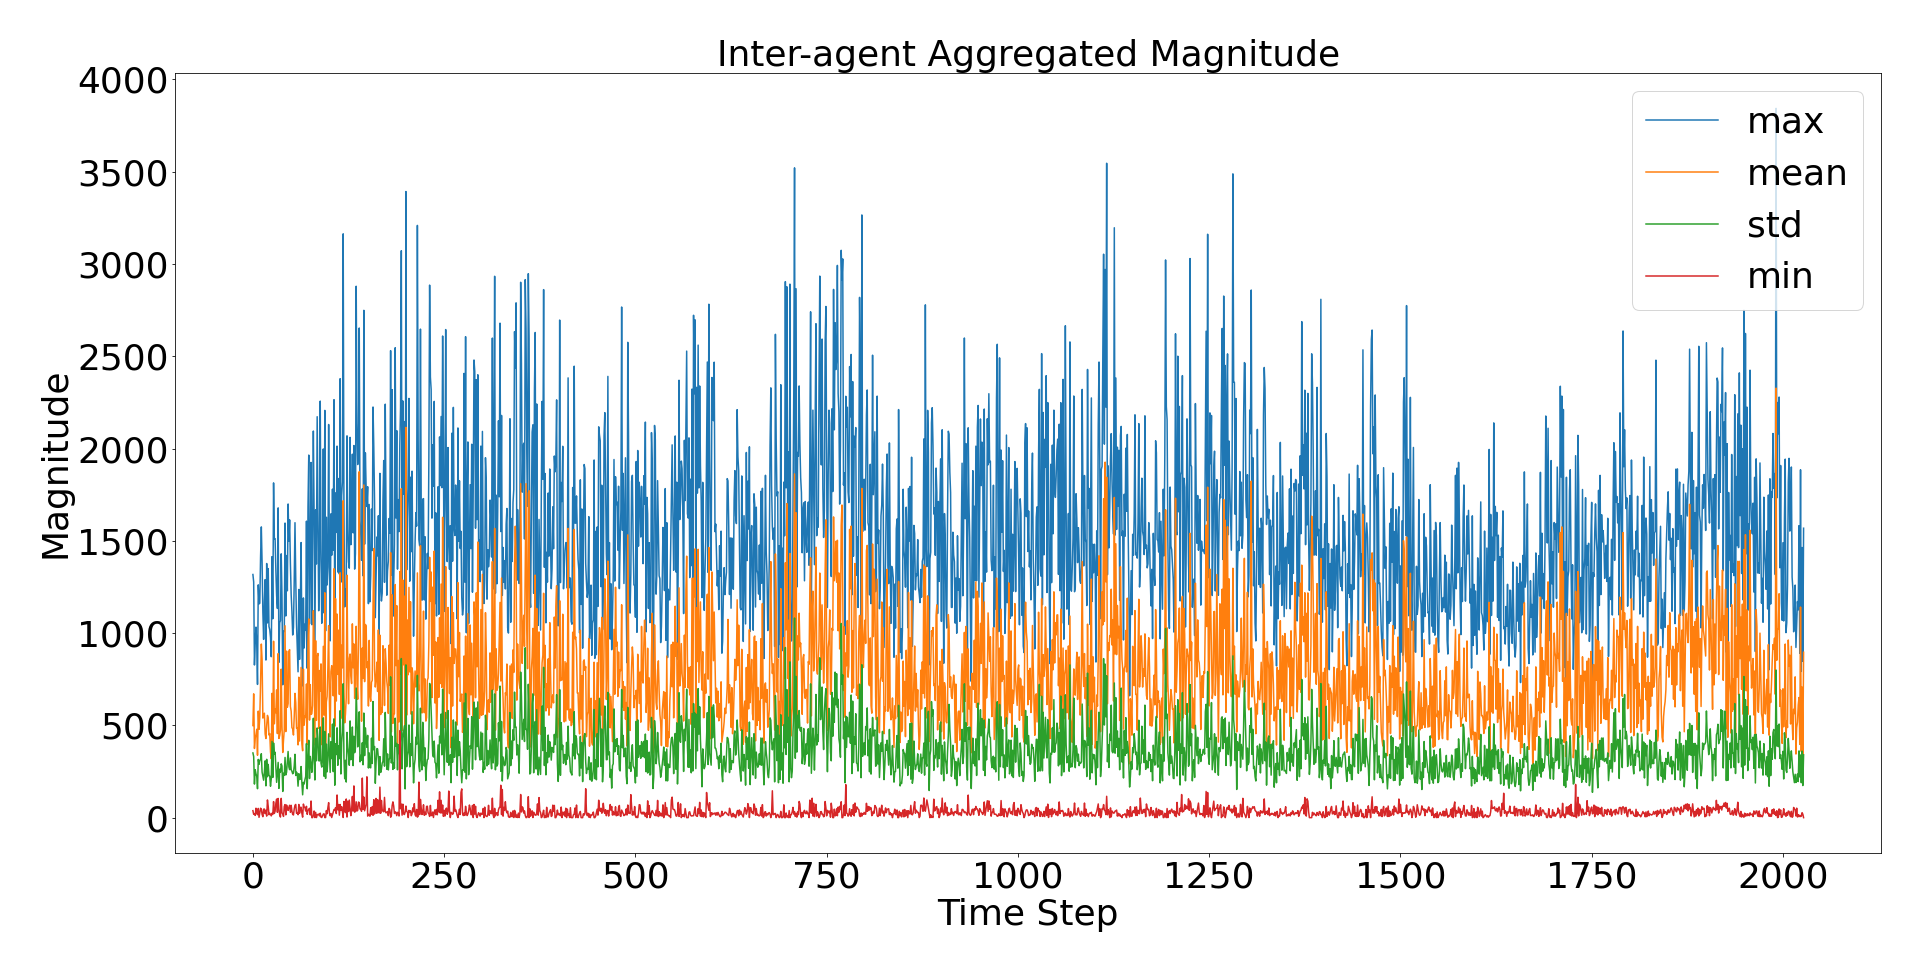
\includegraphics[width=8cm]{figures/baselineSwarmMagnitude1}
	\end{center}
	\caption{Baseline swarm in with compression set 1. \label{fig:baselineSwarmMagnitude1}}
\end{figure}

\begin{figure}[H]
	\begin{center}
		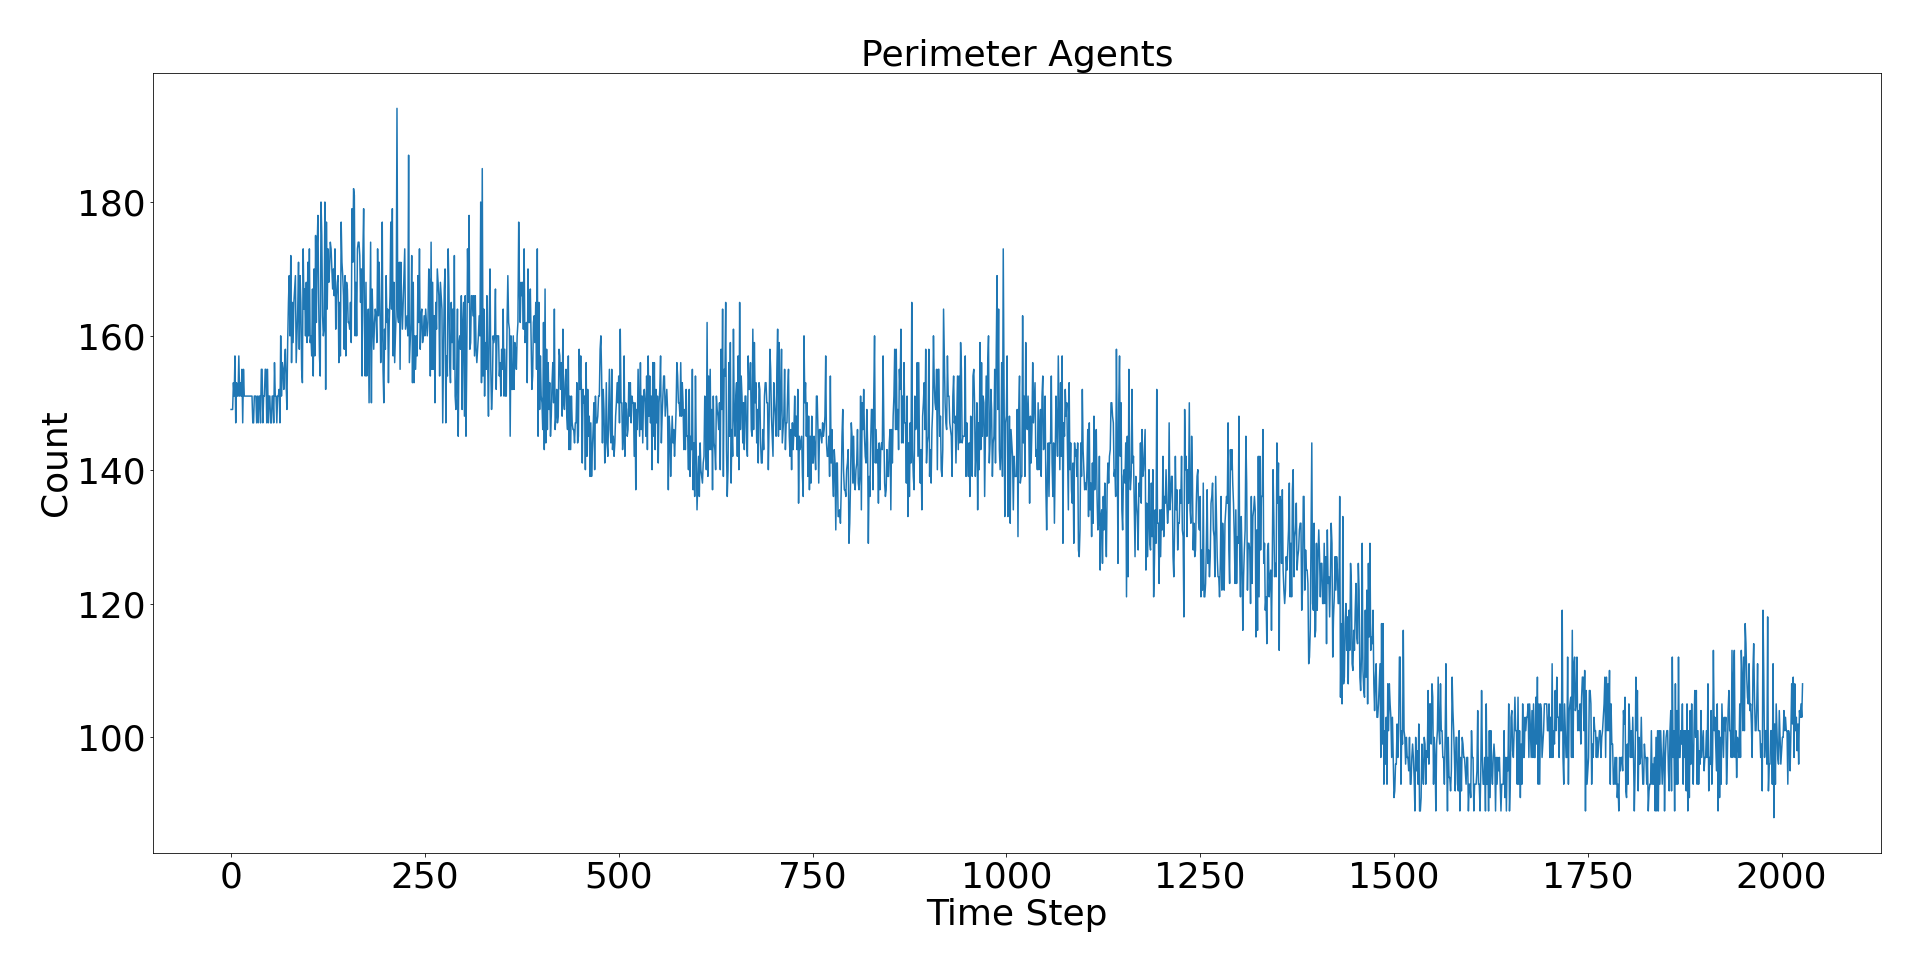
\includegraphics[width=8cm]{figures/baselineSwarmPerimeter1}
	\end{center}
	\caption{Baseline swarm in with compression set 1. \label{fig:baselineSwarmPerimeter1}}
\end{figure}

\begin{figure}[H]
	\begin{center}
		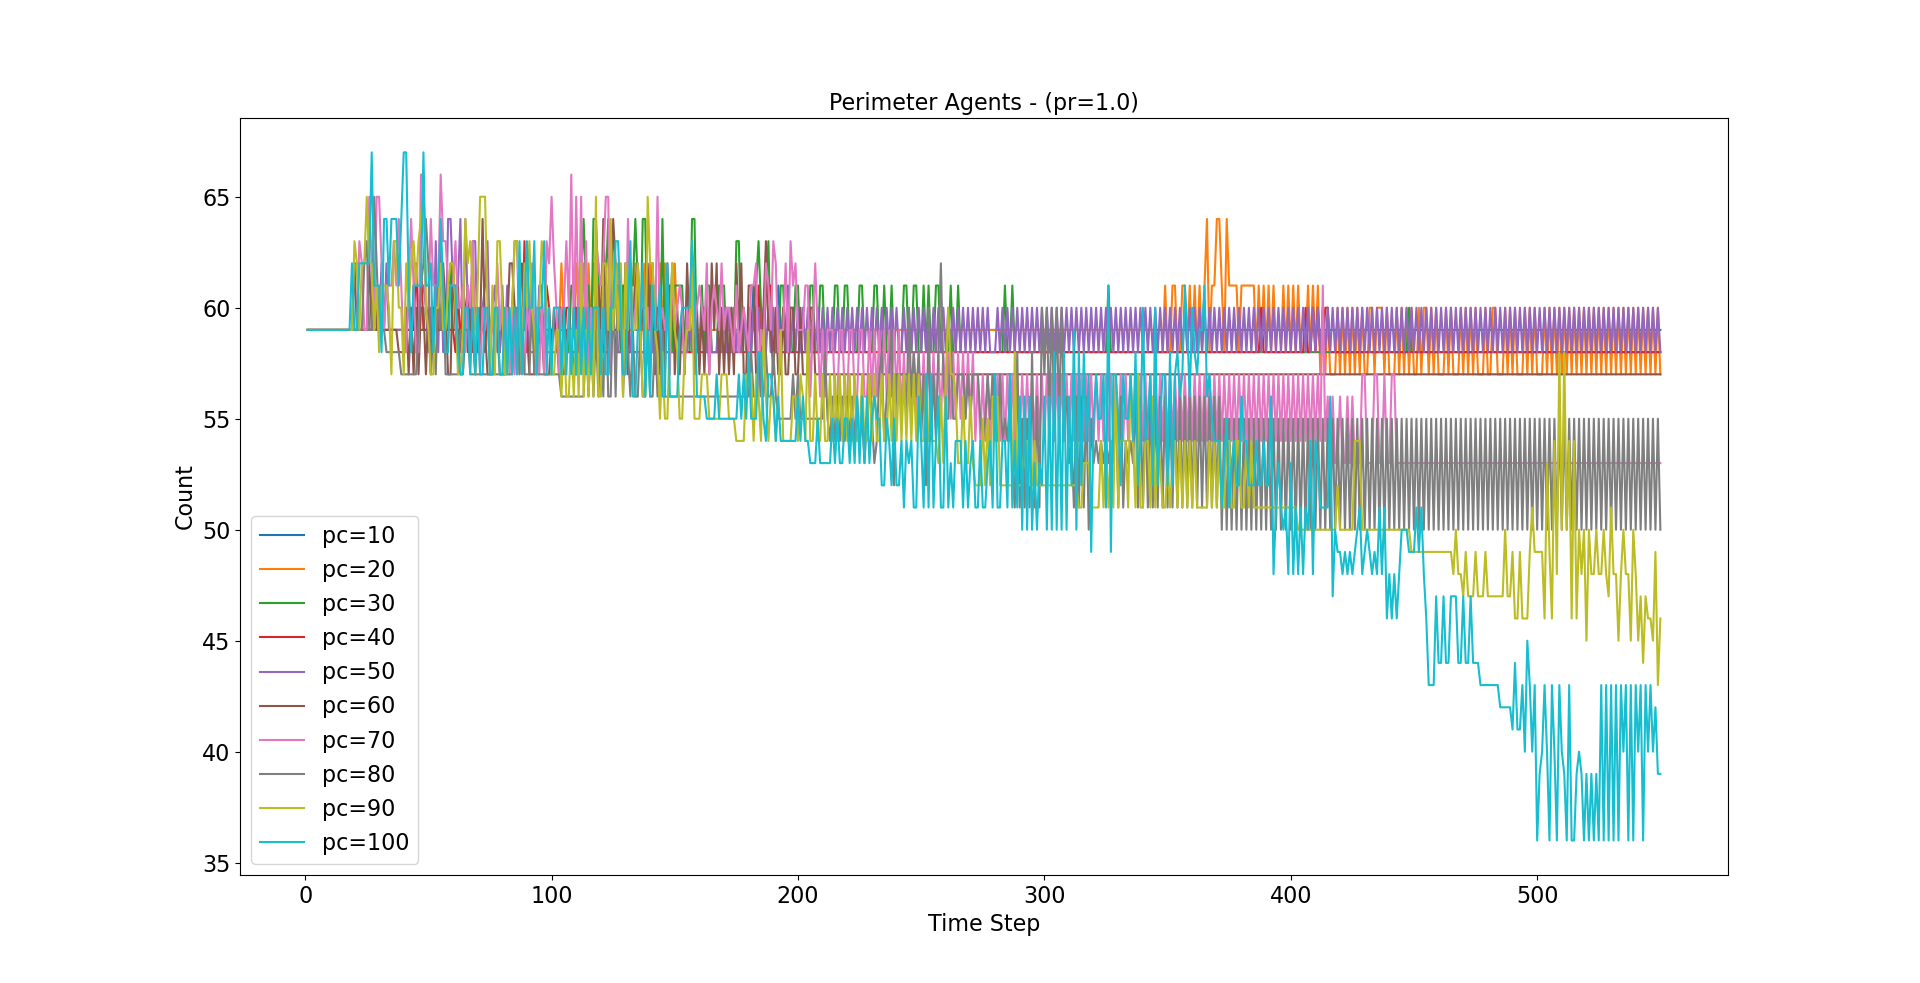
\includegraphics[width=9cm]{figures/Figure_1}
	\end{center}
	\caption{Sample}
\end{figure}
\begin{figure}[H]
	\begin{center}
		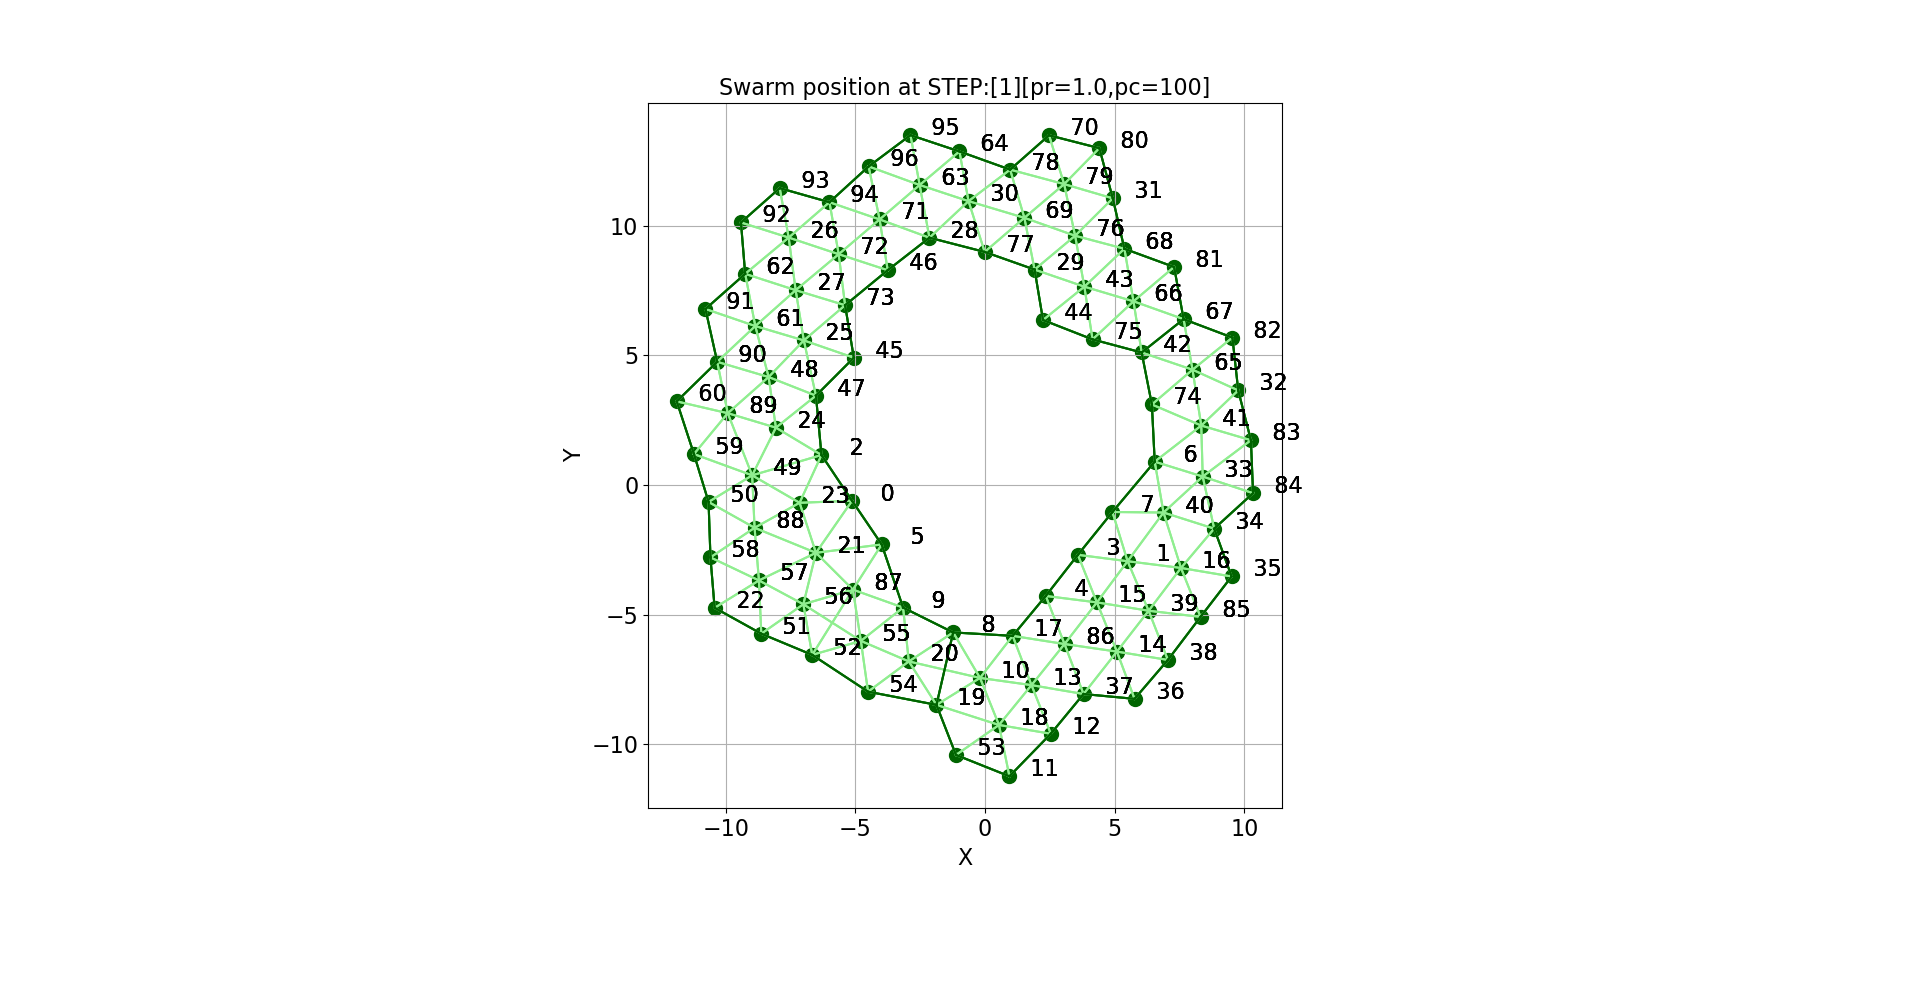
\includegraphics[width=9cm]{figures/Figure_2}
	\end{center}
	\caption{Sample}
\end{figure}
\begin{figure}[H]
	\begin{center}
		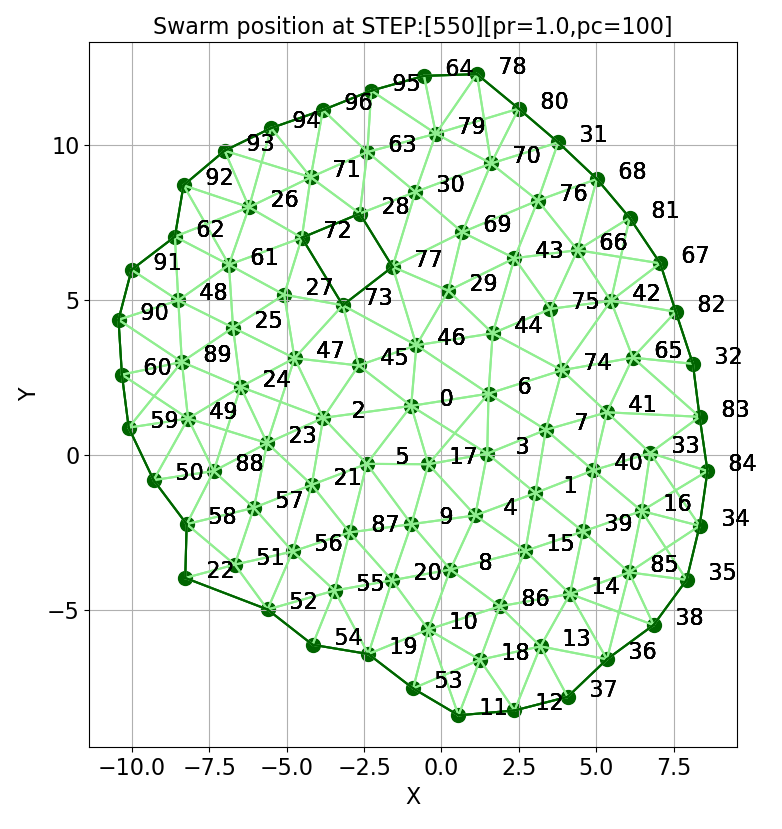
\includegraphics[width=9cm]{figures/Figure_3}
	\end{center}
	\caption{Sample}
\end{figure}
\begin{figure}[H]
	\begin{center}
		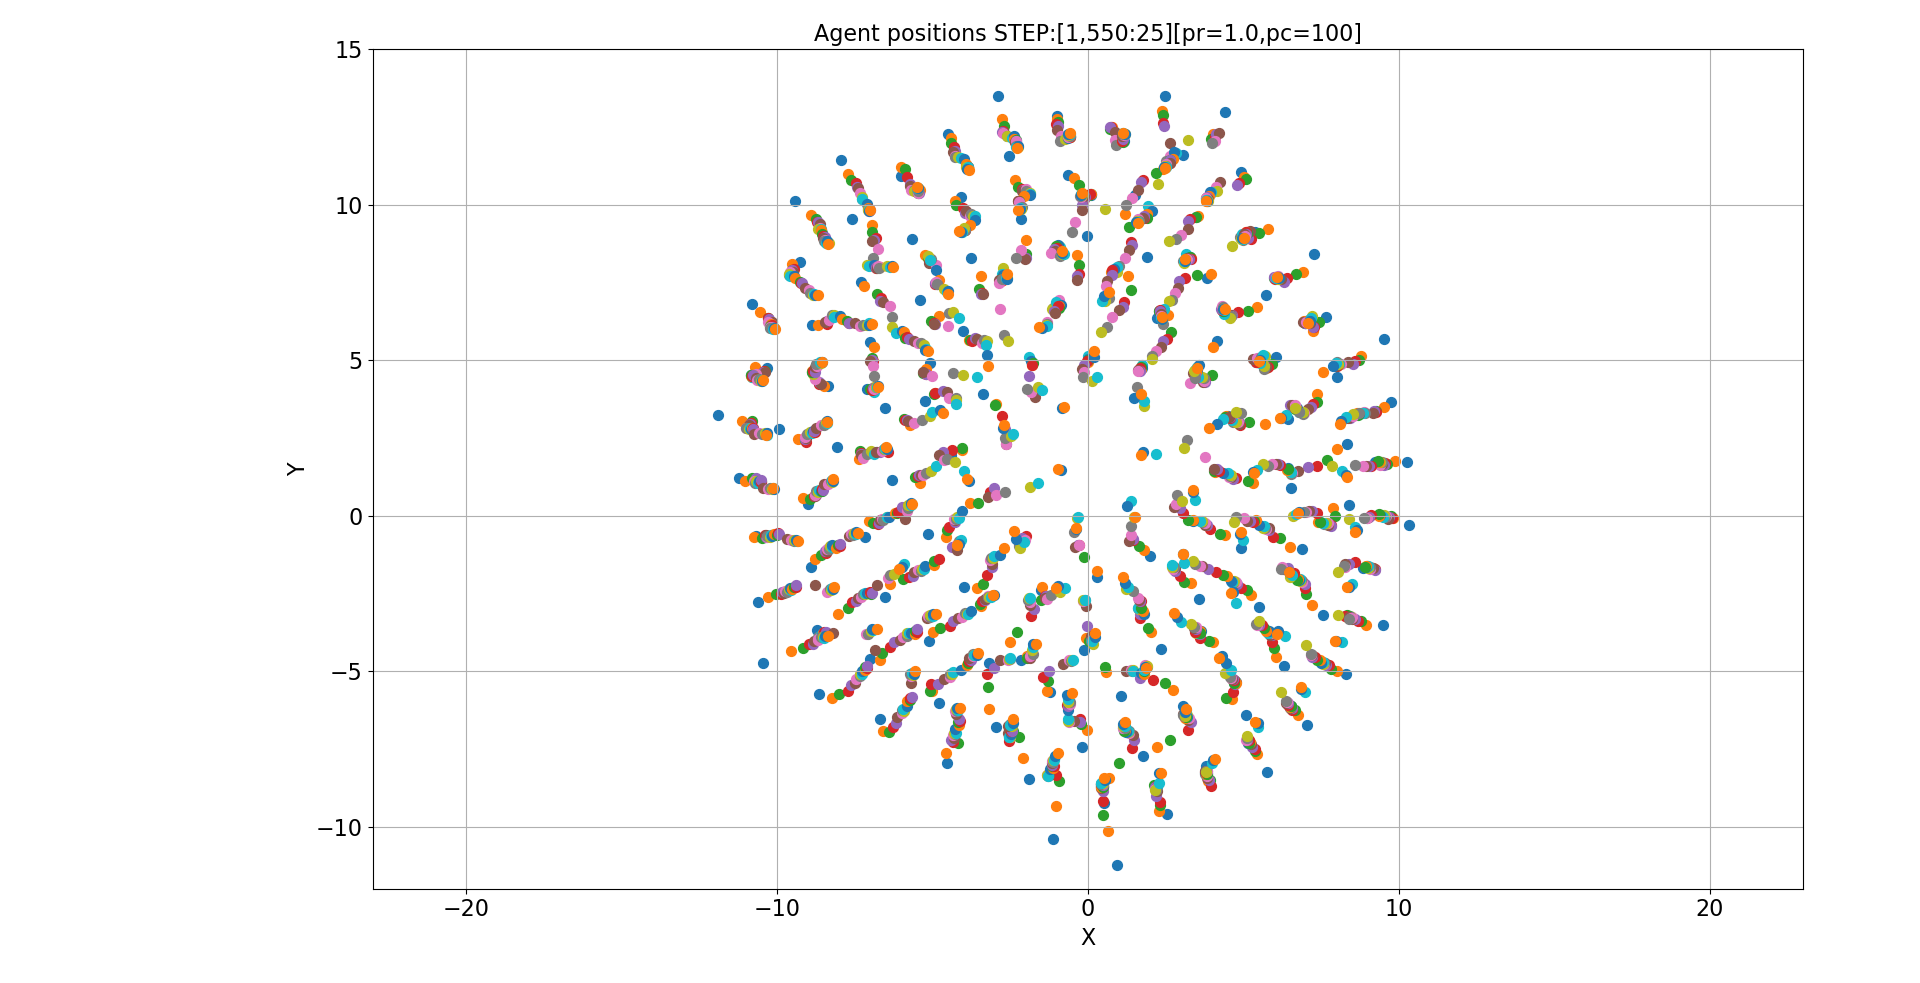
\includegraphics[width=9cm]{figures/Figure_4}
	\end{center}
	\caption{Sample}
\end{figure}
\begin{figure}[H]
	\begin{center}
		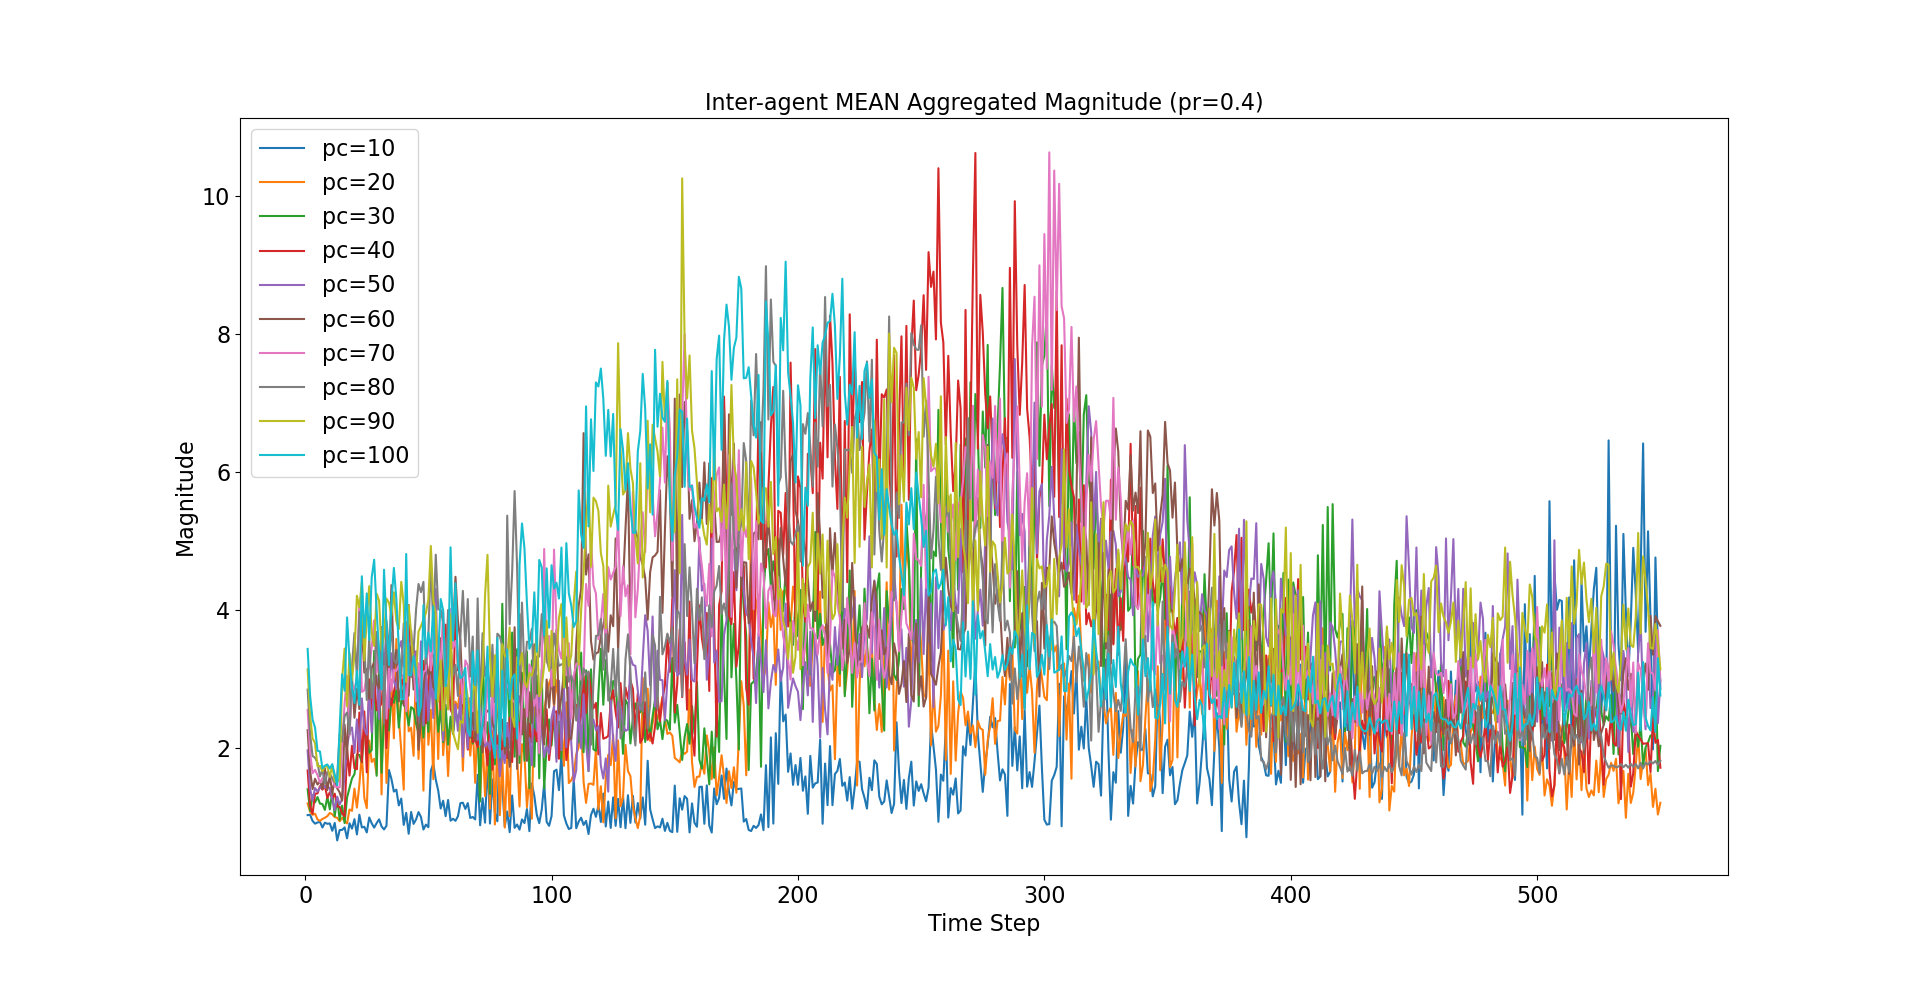
\includegraphics[width=9cm]{figures/Figure_5}
	\end{center}
	\caption{Sample}
\end{figure}
\begin{figure}[H]
	\begin{center}
		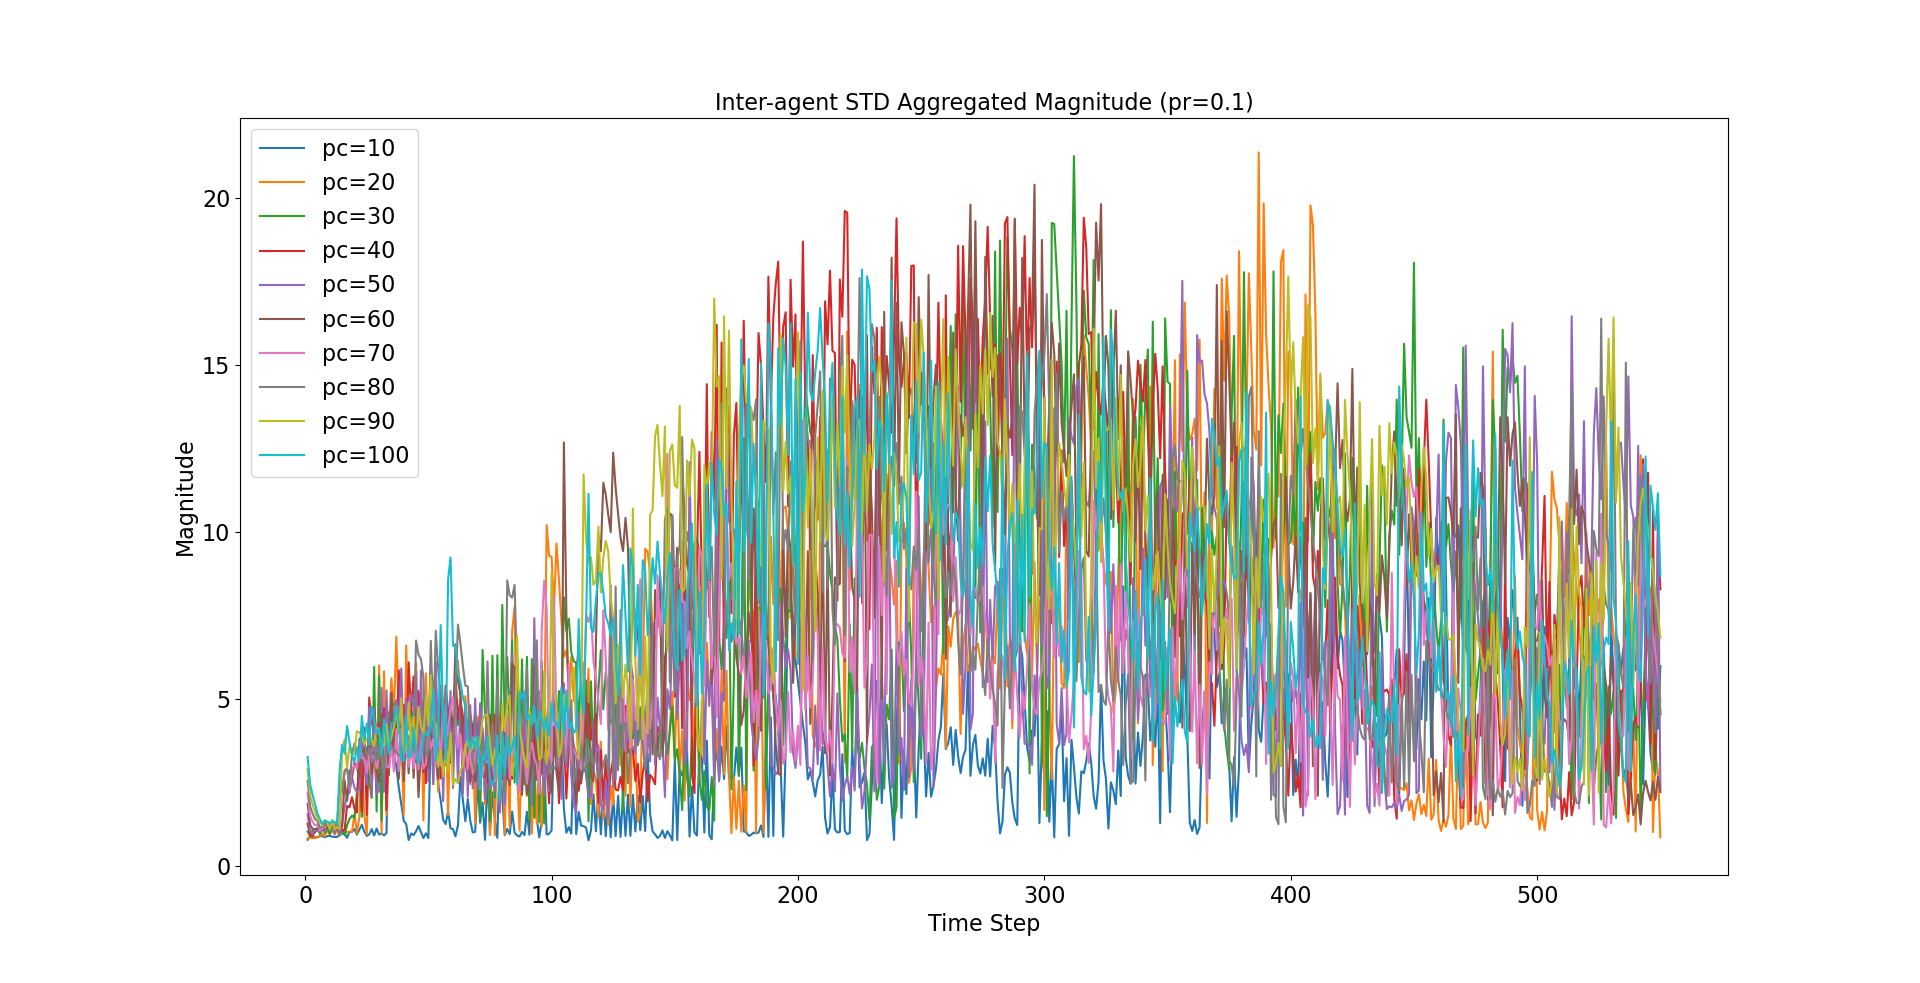
\includegraphics[width=9cm]{figures/Figure_6}
	\end{center}
	\caption{Sample}
\end{figure}
\begin{figure}[H]
	\begin{center}
		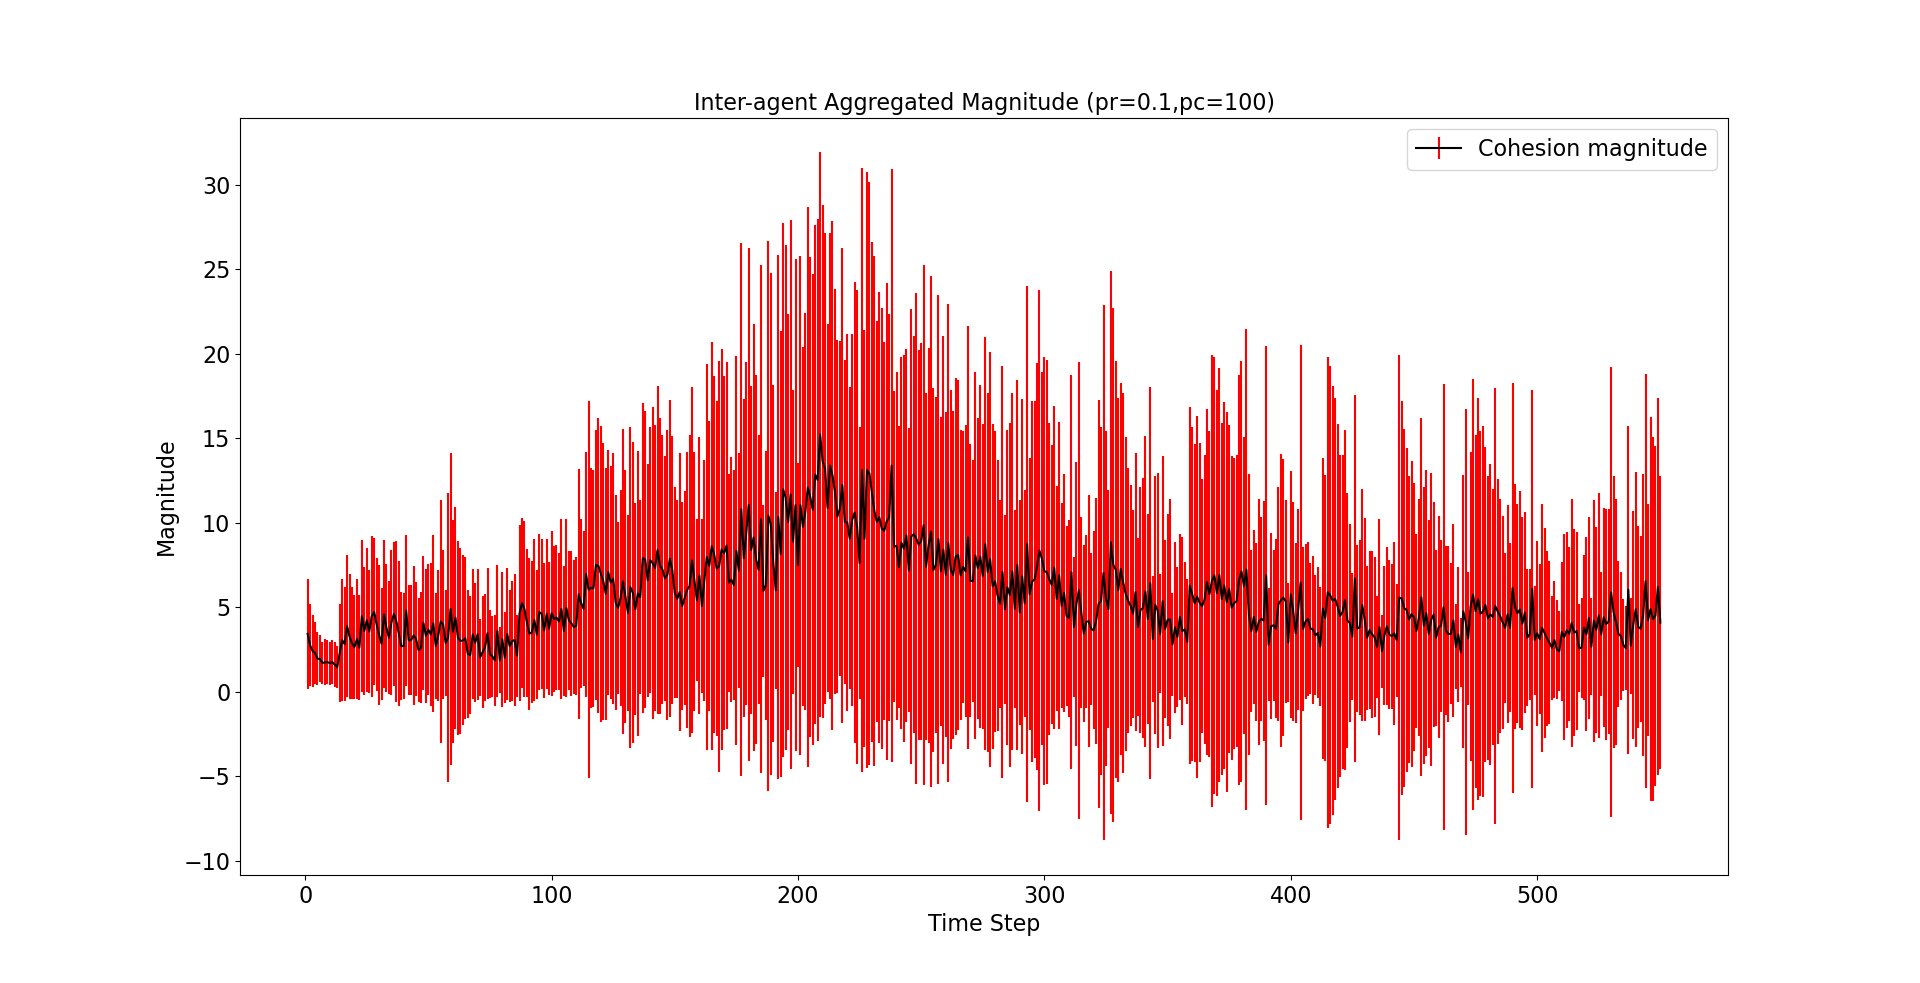
\includegraphics[width=9cm]{figures/Figure_7}
	\end{center}
	\caption{Sample}
\end{figure}
\begin{figure}[H]
	\begin{center}
		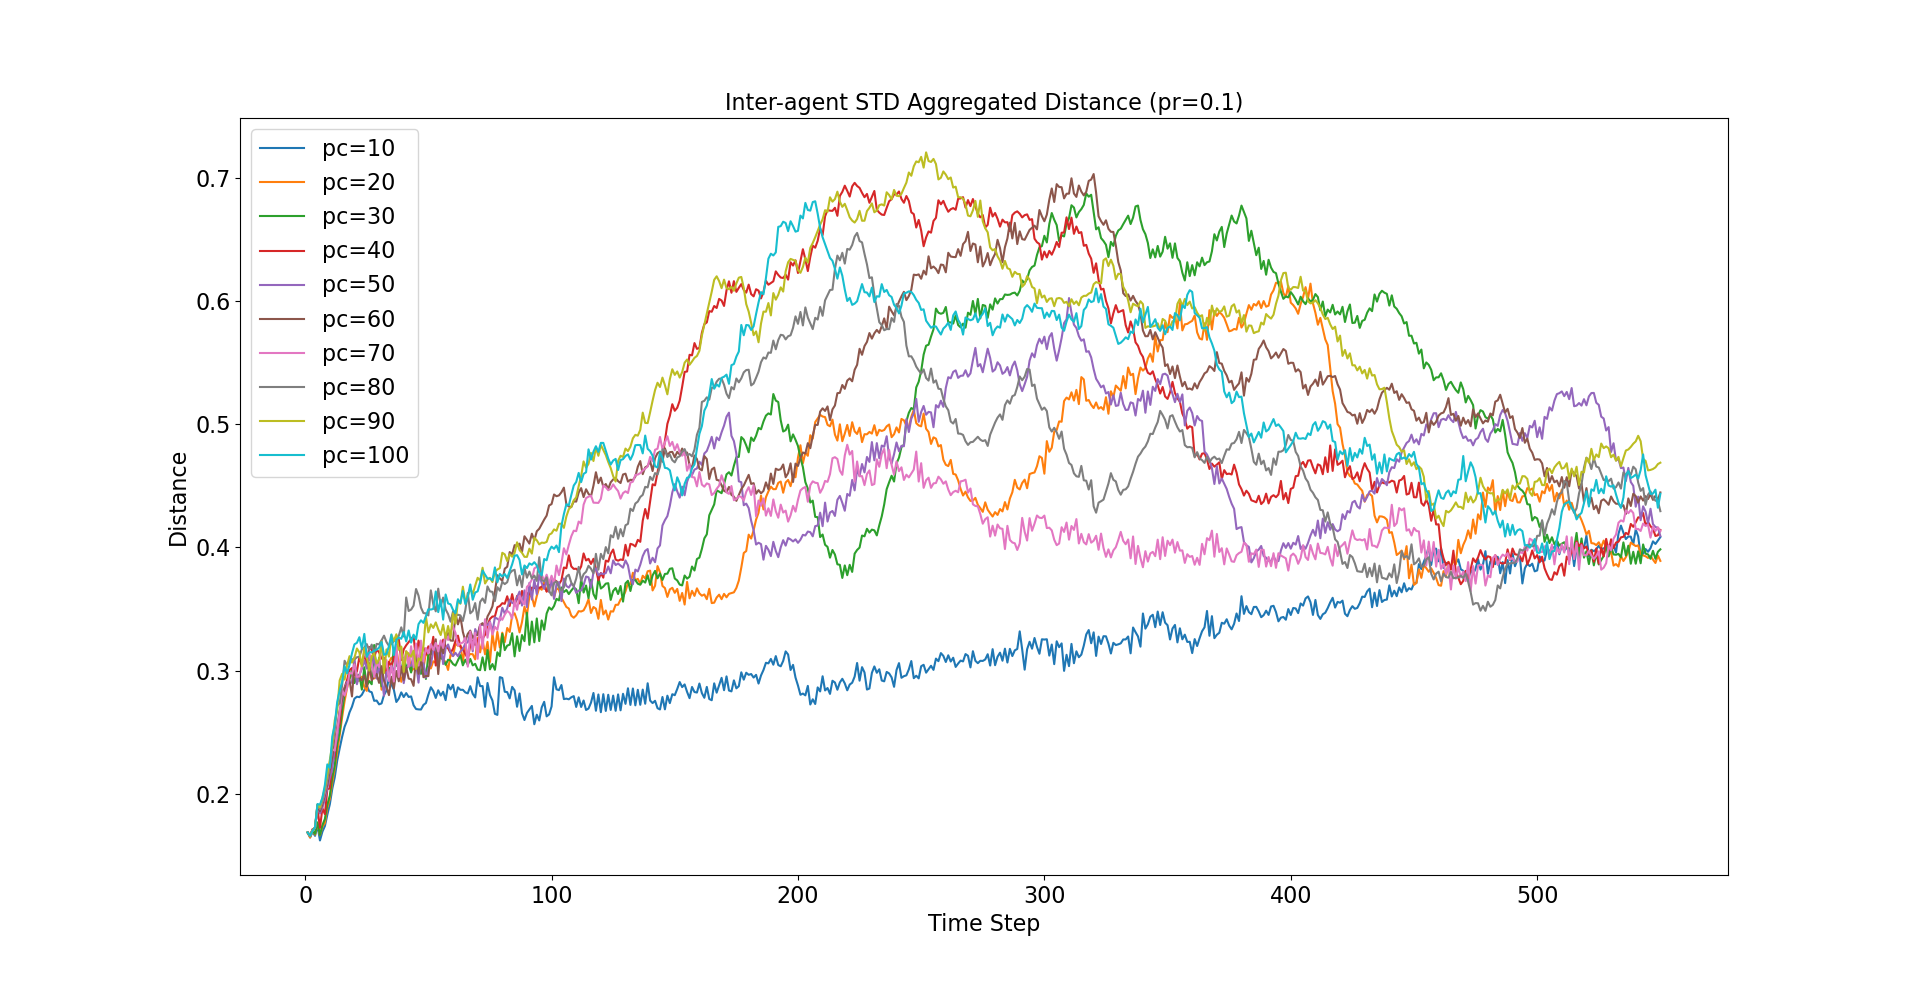
\includegraphics[width=9cm]{figures/Figure_8}
	\end{center}
	\caption{Sample}
\end{figure}
\begin{figure}[H]
	\begin{center}
		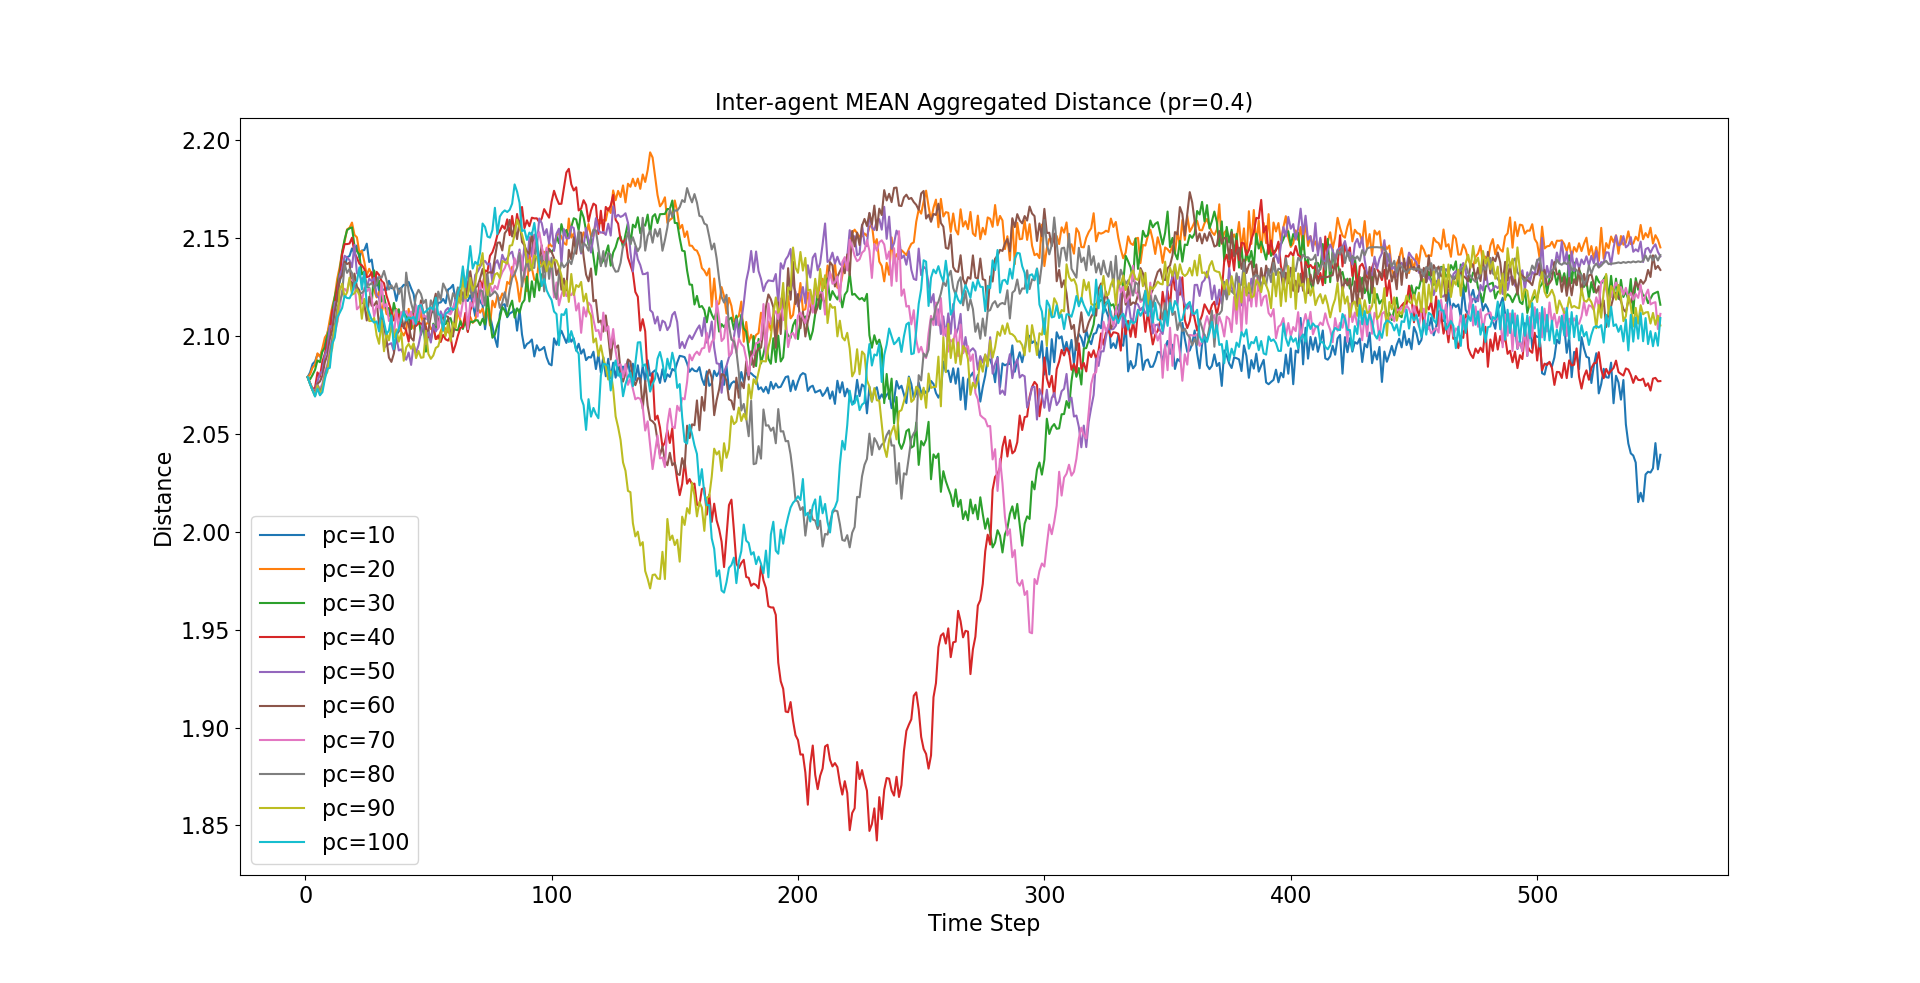
\includegraphics[width=9cm]{figures/Figure_9}
	\end{center}
	\caption{Sample}
\end{figure}
\begin{figure}[H]
	\begin{center}
		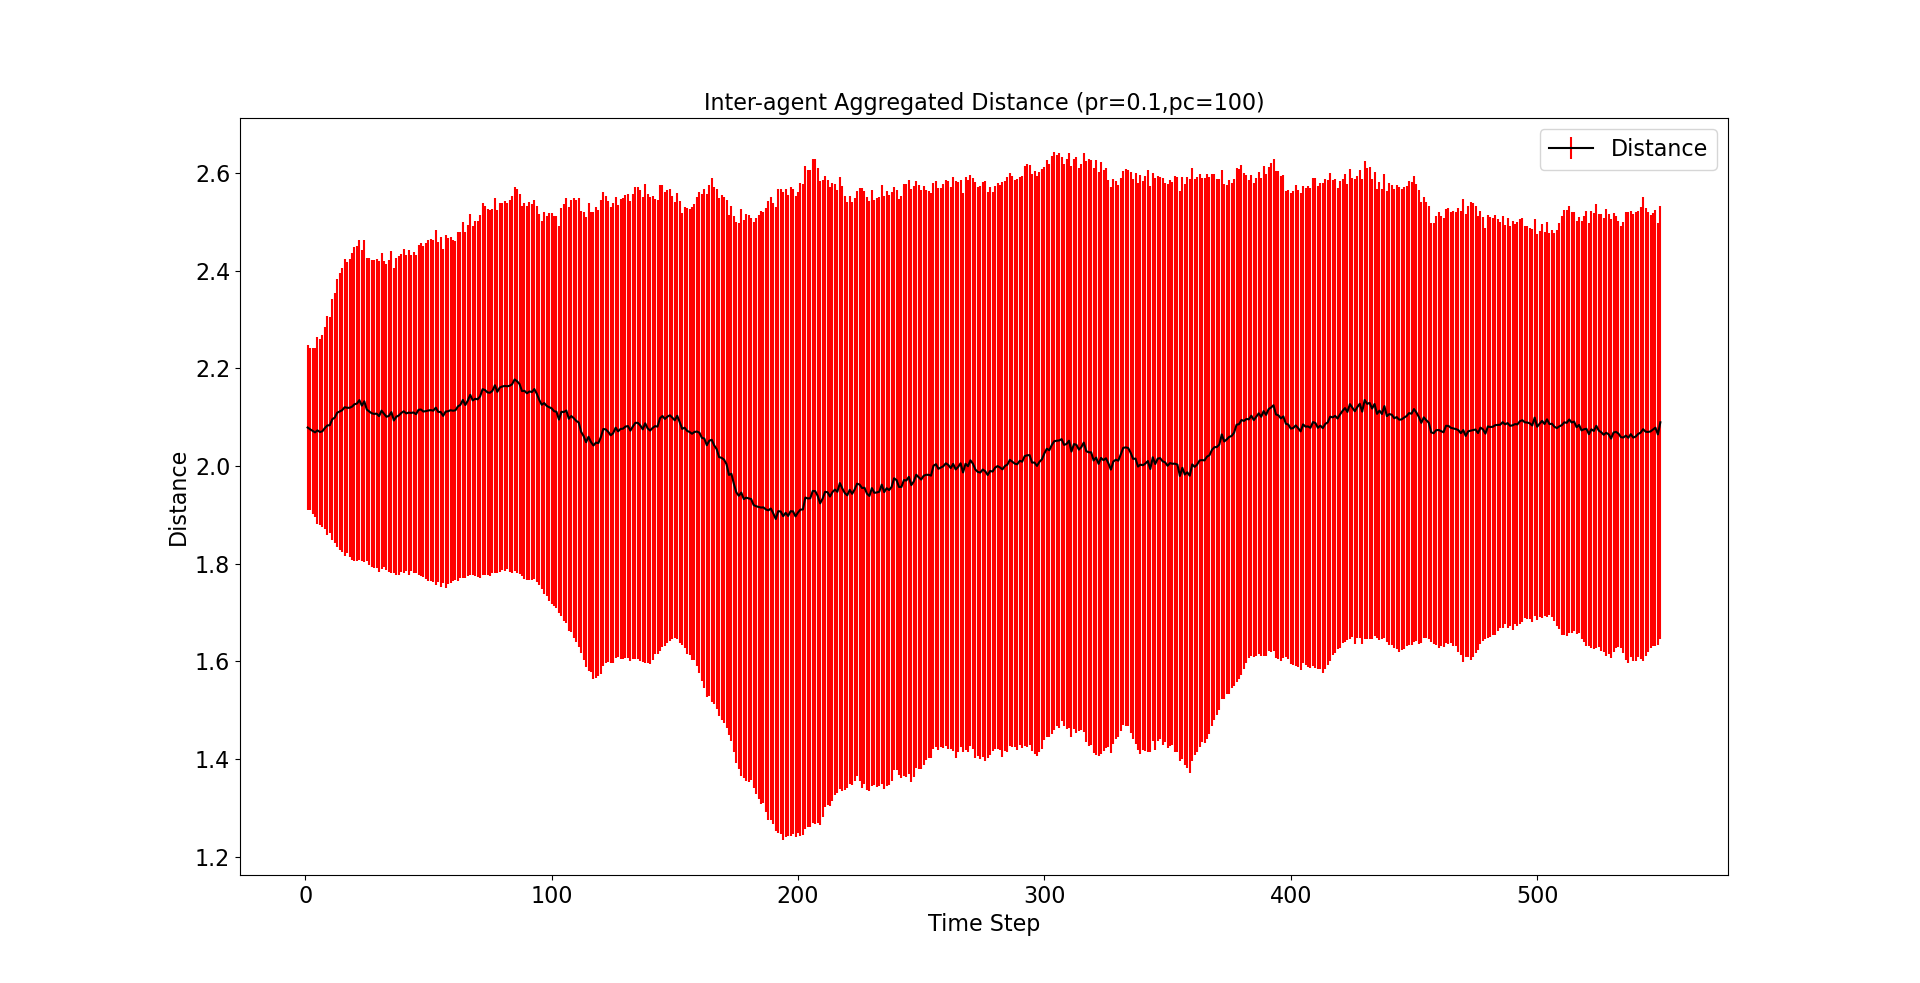
\includegraphics[width=9cm]{figures/Figure_10}
	\end{center}
	\caption{Sample}
\end{figure}

\begin{figure}[H]
	\begin{center}
		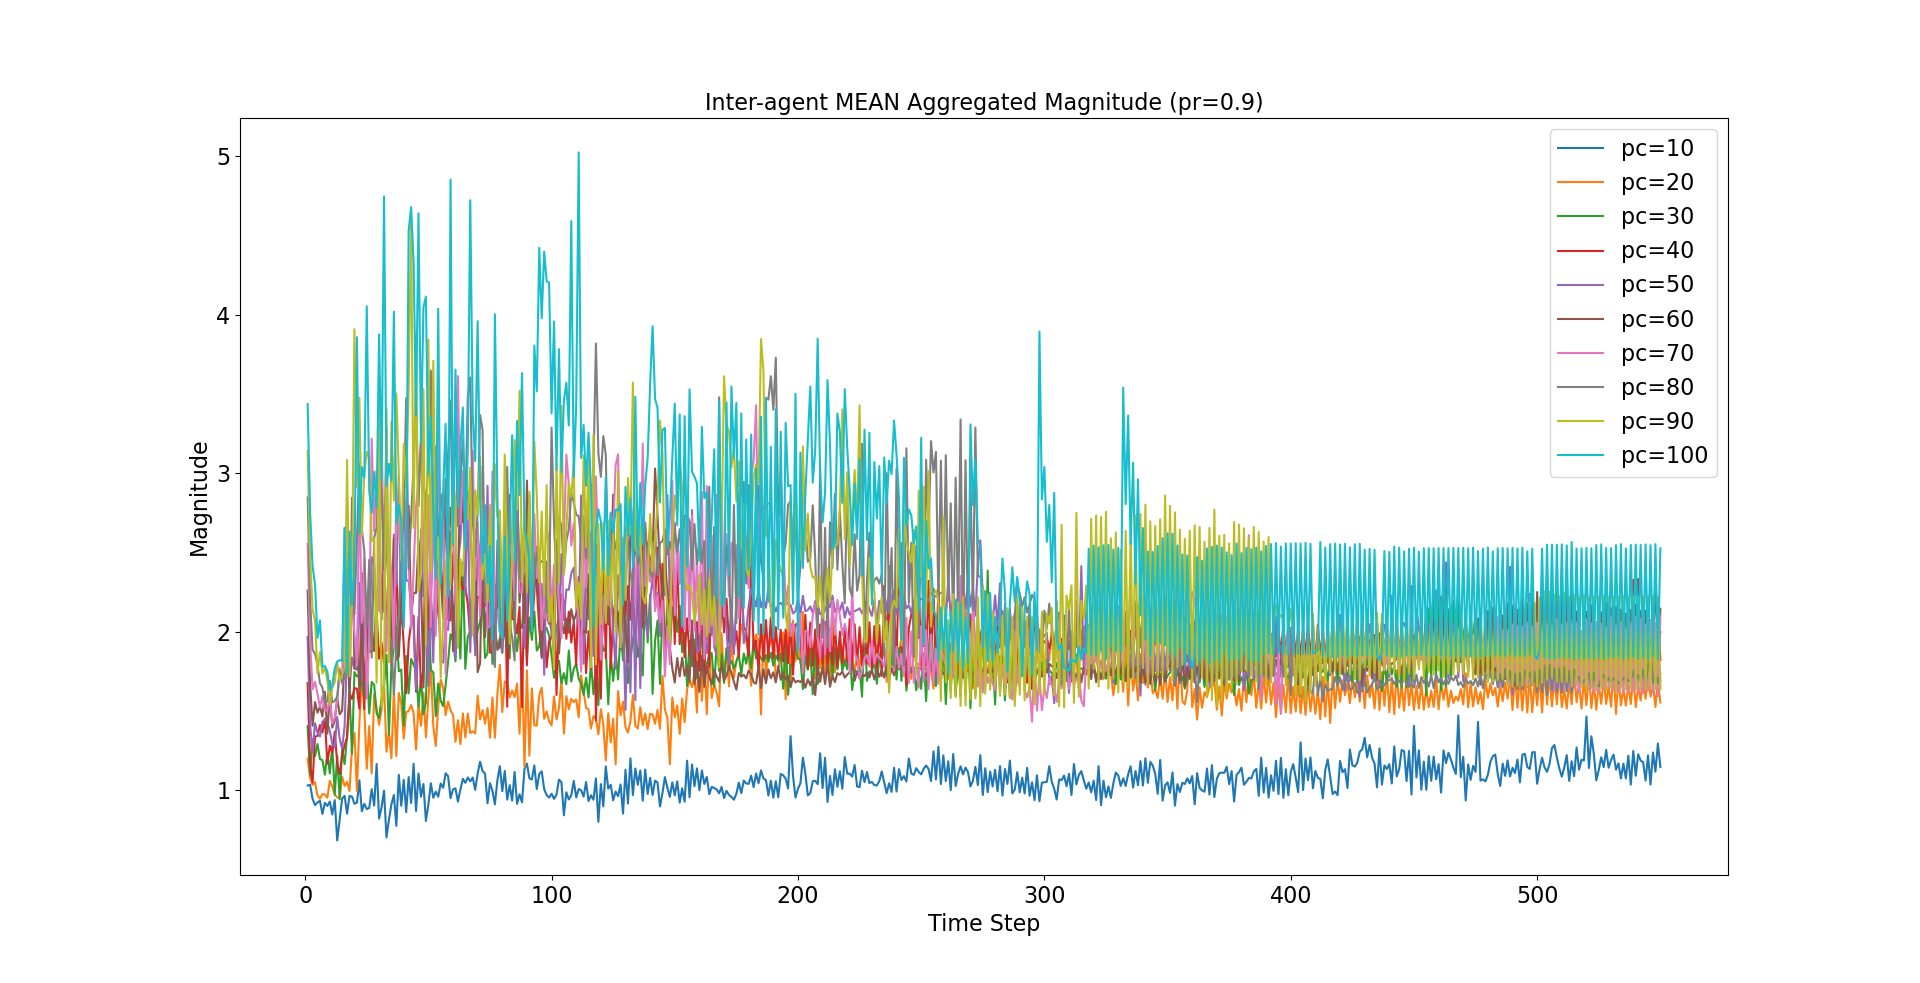
\includegraphics[width=9cm]{figures/mag-pr-0.9-mean}
	\end{center}
	\caption{MAG pr=0.9 mean}
\end{figure}

\begin{figure}[H]
	\begin{center}
		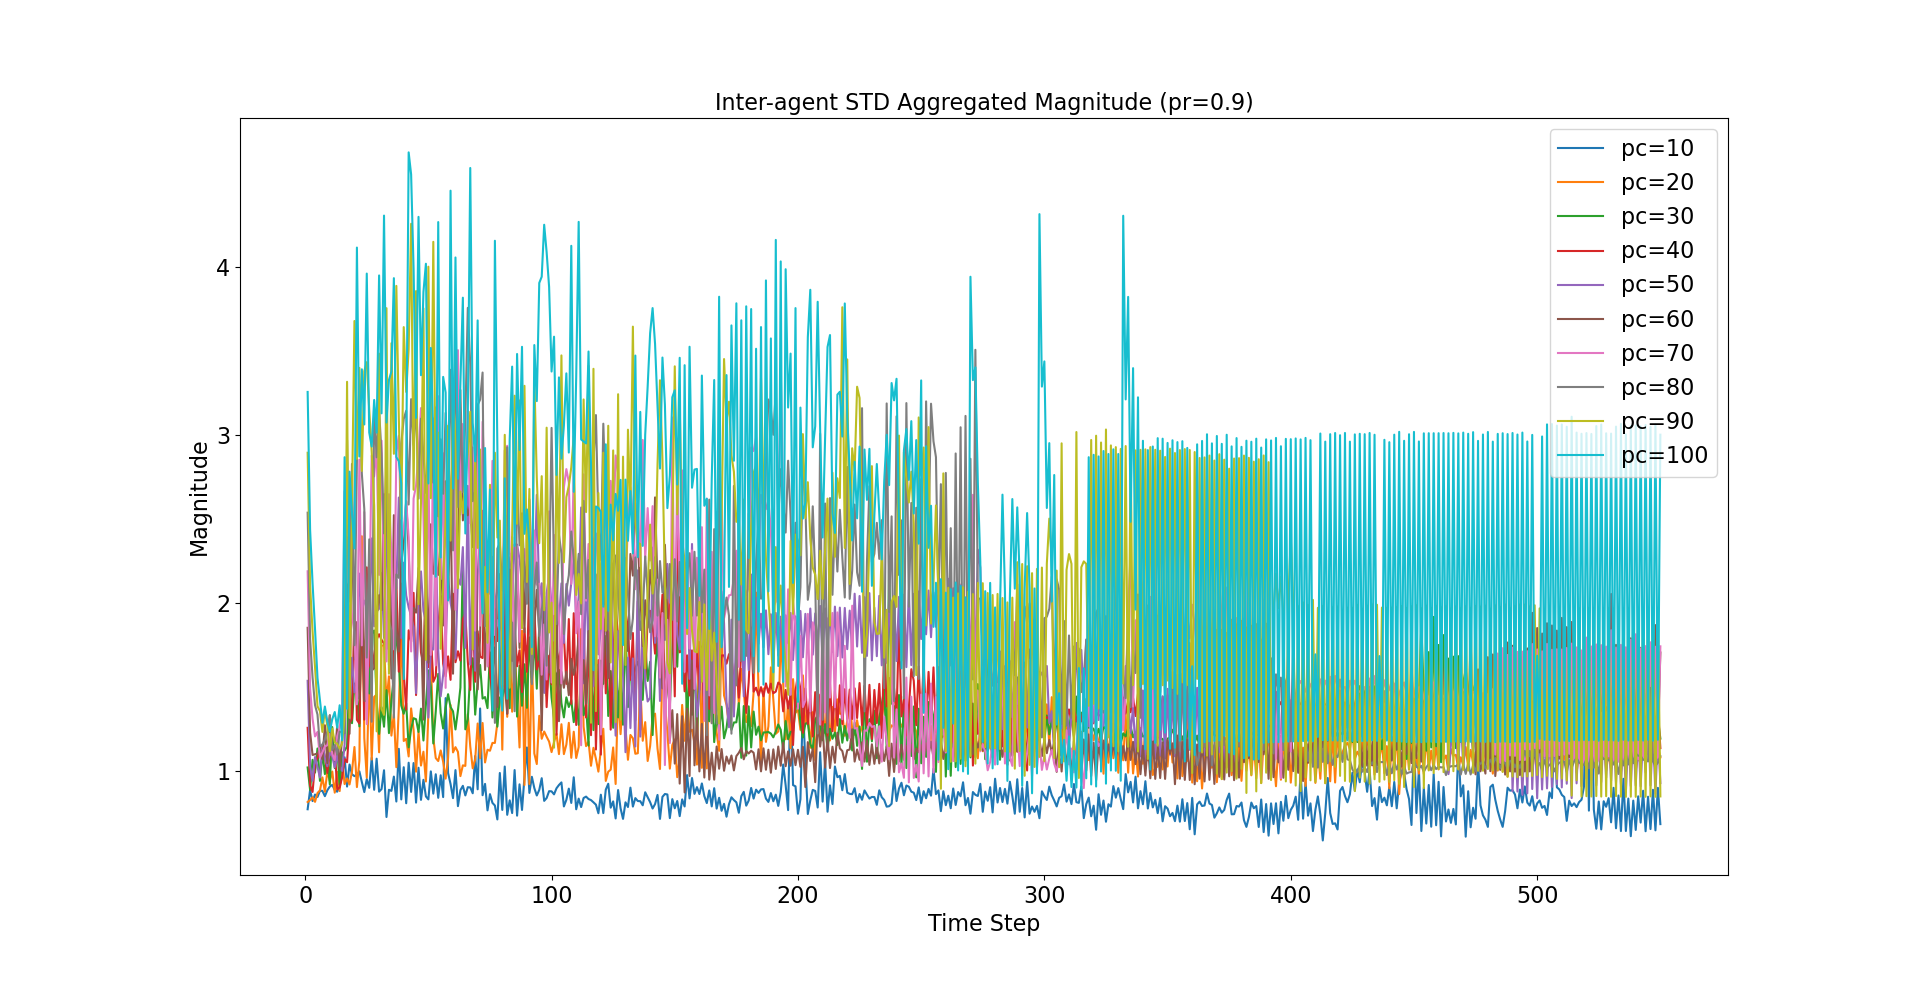
\includegraphics[width=9cm]{figures/mag-pr-0.9-std}
	\end{center}
	\caption{MAG pr=0.9 std}
\end{figure}

\begin{figure}[H]
	\begin{center}
		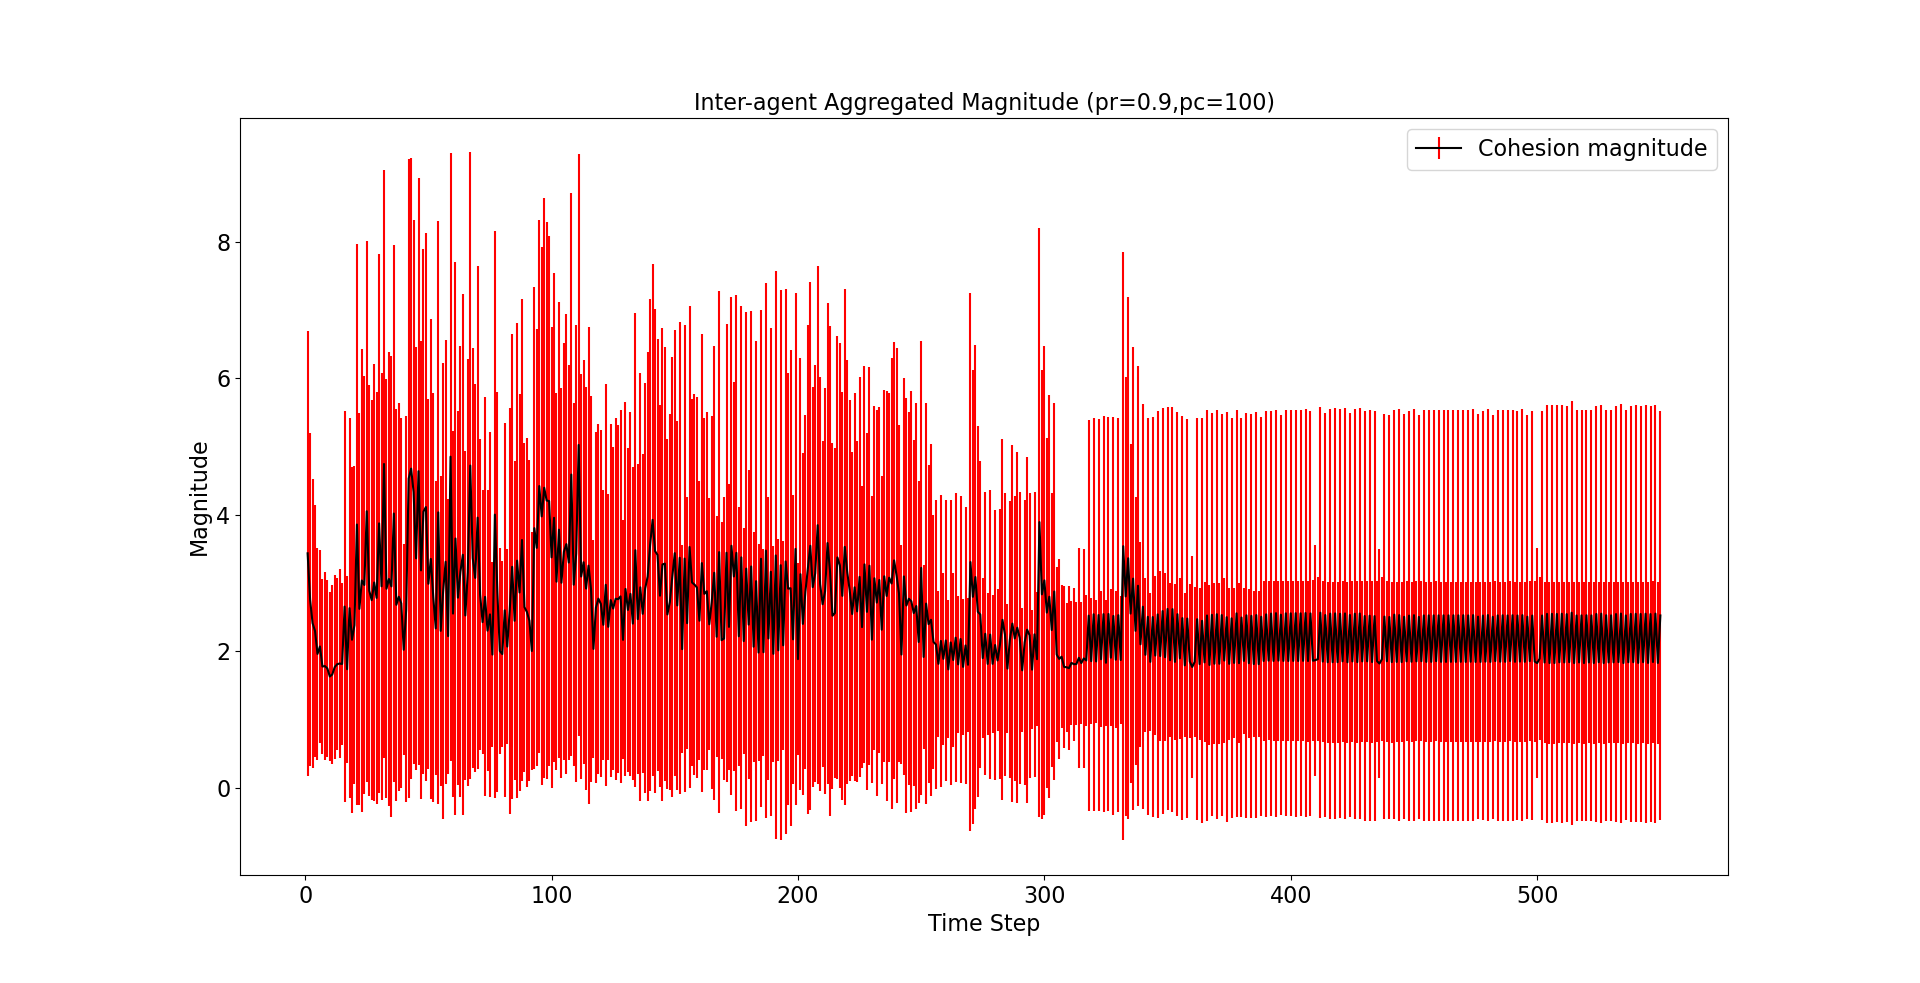
\includegraphics[width=9cm]{figures/mag-pr-0.9-pc-100-error}
	\end{center}
	\caption{MAG pr=0.9 pc=100 error}
\end{figure}

\begin{figure}[H]
	\begin{center}
		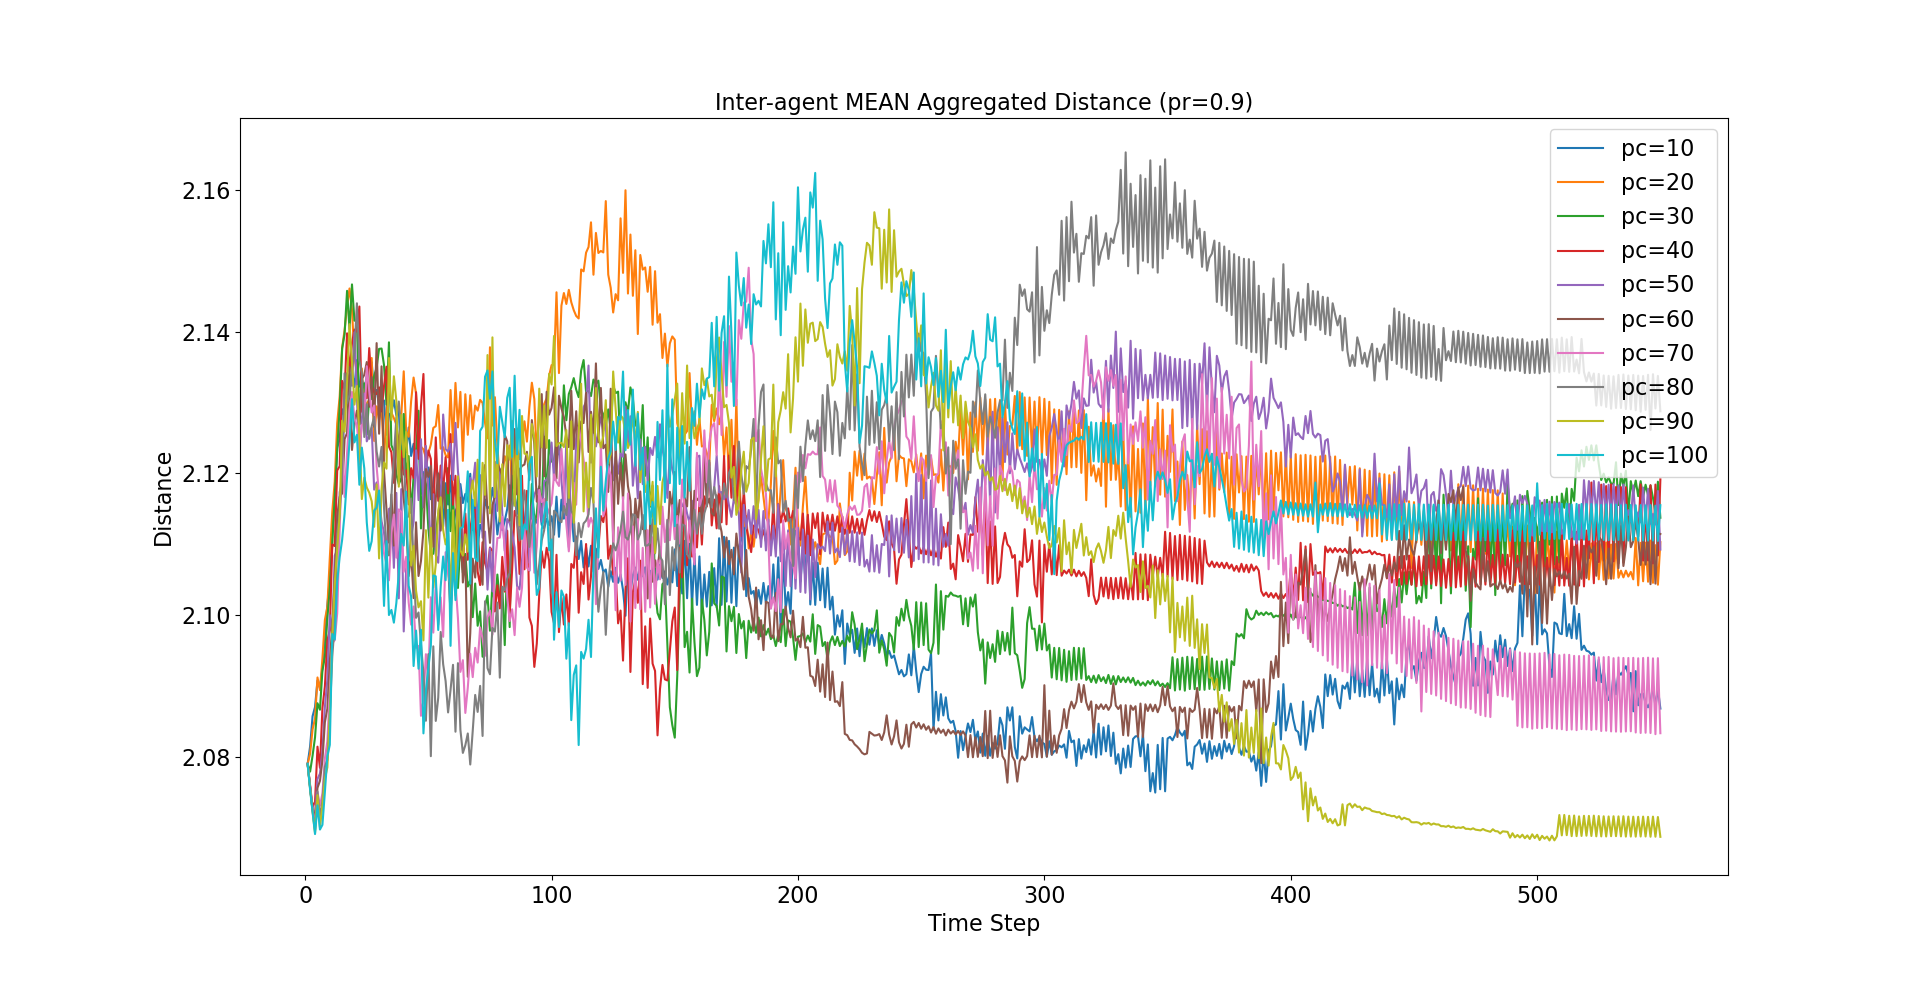
\includegraphics[width=9cm]{figures/dist-pr-0.9-mean}
	\end{center}
	\caption{DIST pr=0.9 mean}
\end{figure}

\begin{figure}[H]
	\begin{center}
		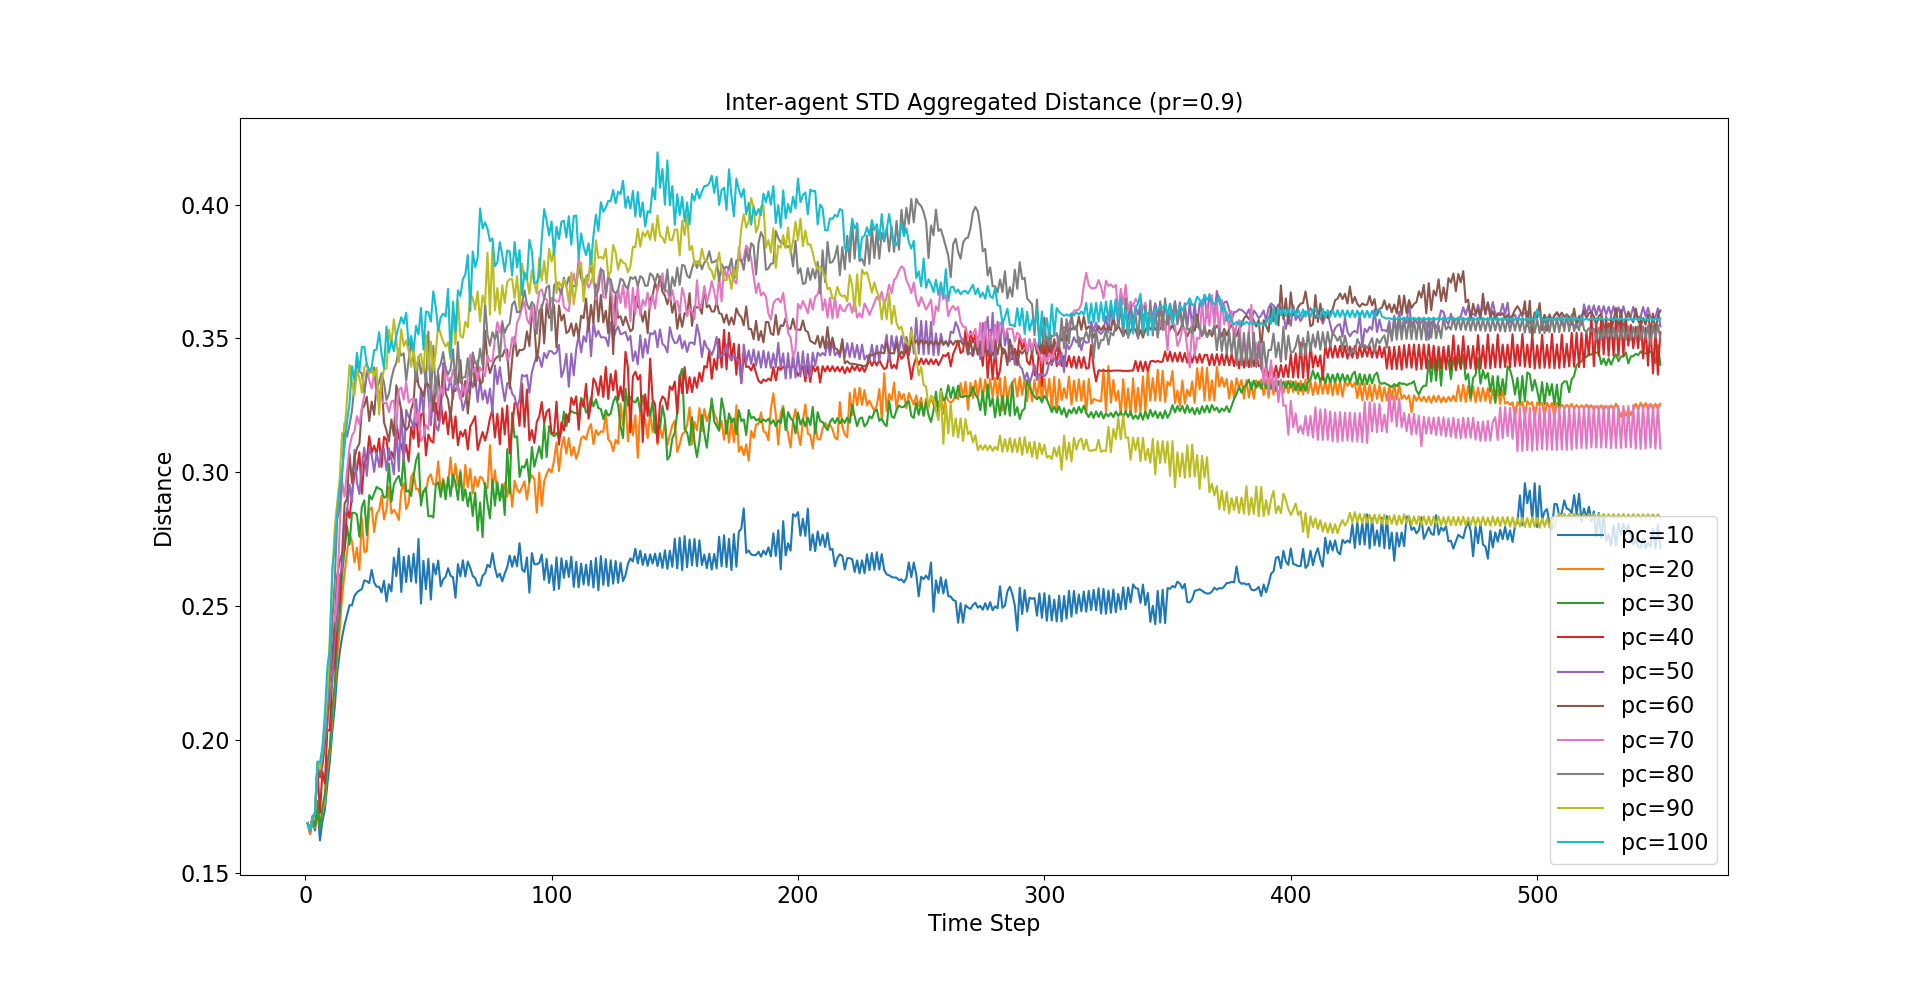
\includegraphics[width=9cm]{figures/dist-pr-0.9-std}
	\end{center}
	\caption{DIST pr=0.9 std}
\end{figure}

\begin{figure}[H]
	\begin{center}
		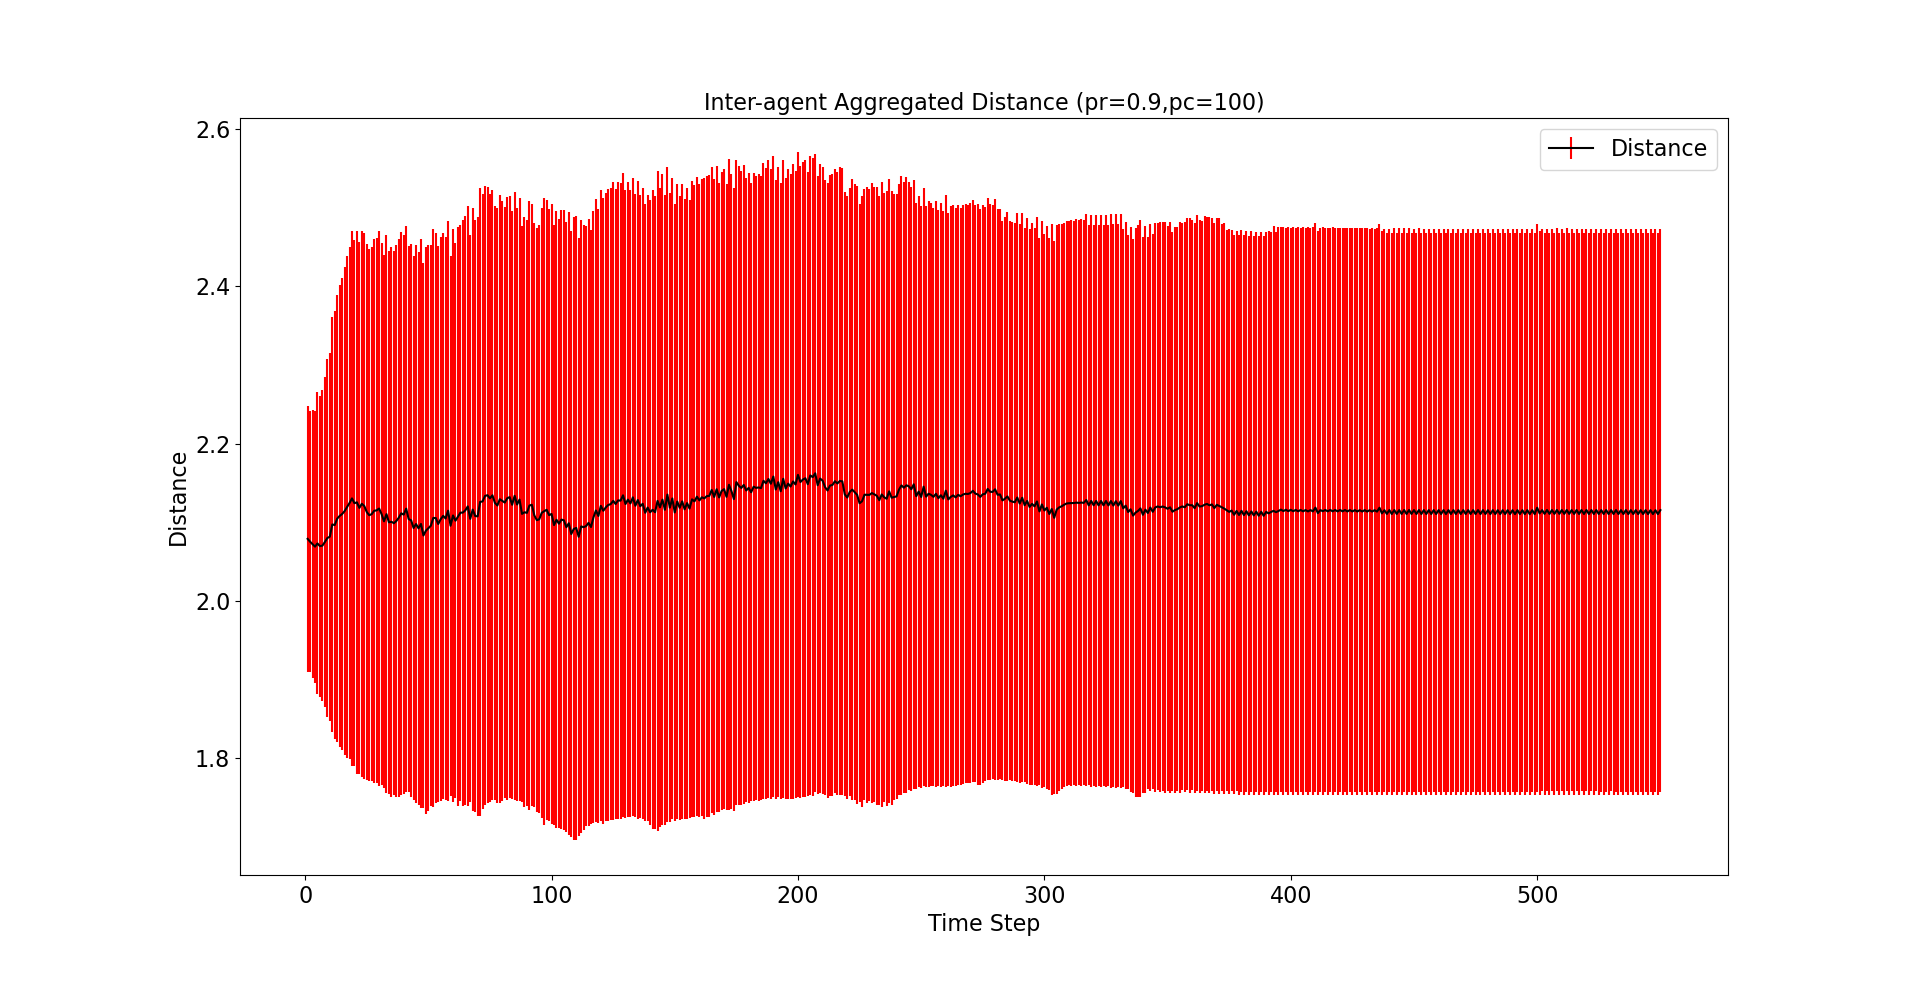
\includegraphics[width=9cm]{figures/dist-pr-0.9-pc-100-error}
	\end{center}
	\caption{DIST pr=0.9 pc=100 error }
\end{figure}


\subsection{Comparison}

\section{Conclusions}\label{conclusions}
From the initial simulations it is possible to show that the technique is able to successfully remove voids and surround an obstacle as shown in the video \href{https://youtu.be/3eY1vvq0JWo}{https://youtu.be/3eY1vvq0JWo}.

\section{Future Work}

\bibliographystyle{abbrv}
\bibliography{perimeter}

\end{document}